\section{Specific requirements}

\subsection{External Interface Requirements}
In this section details about user interfaces, hardware and application programming interfaces are described.

\subsubsection{User Interfaces}
TODO: add an introduction
\begin{figure}[H]
    \centering
    \subfloat[Home]{
        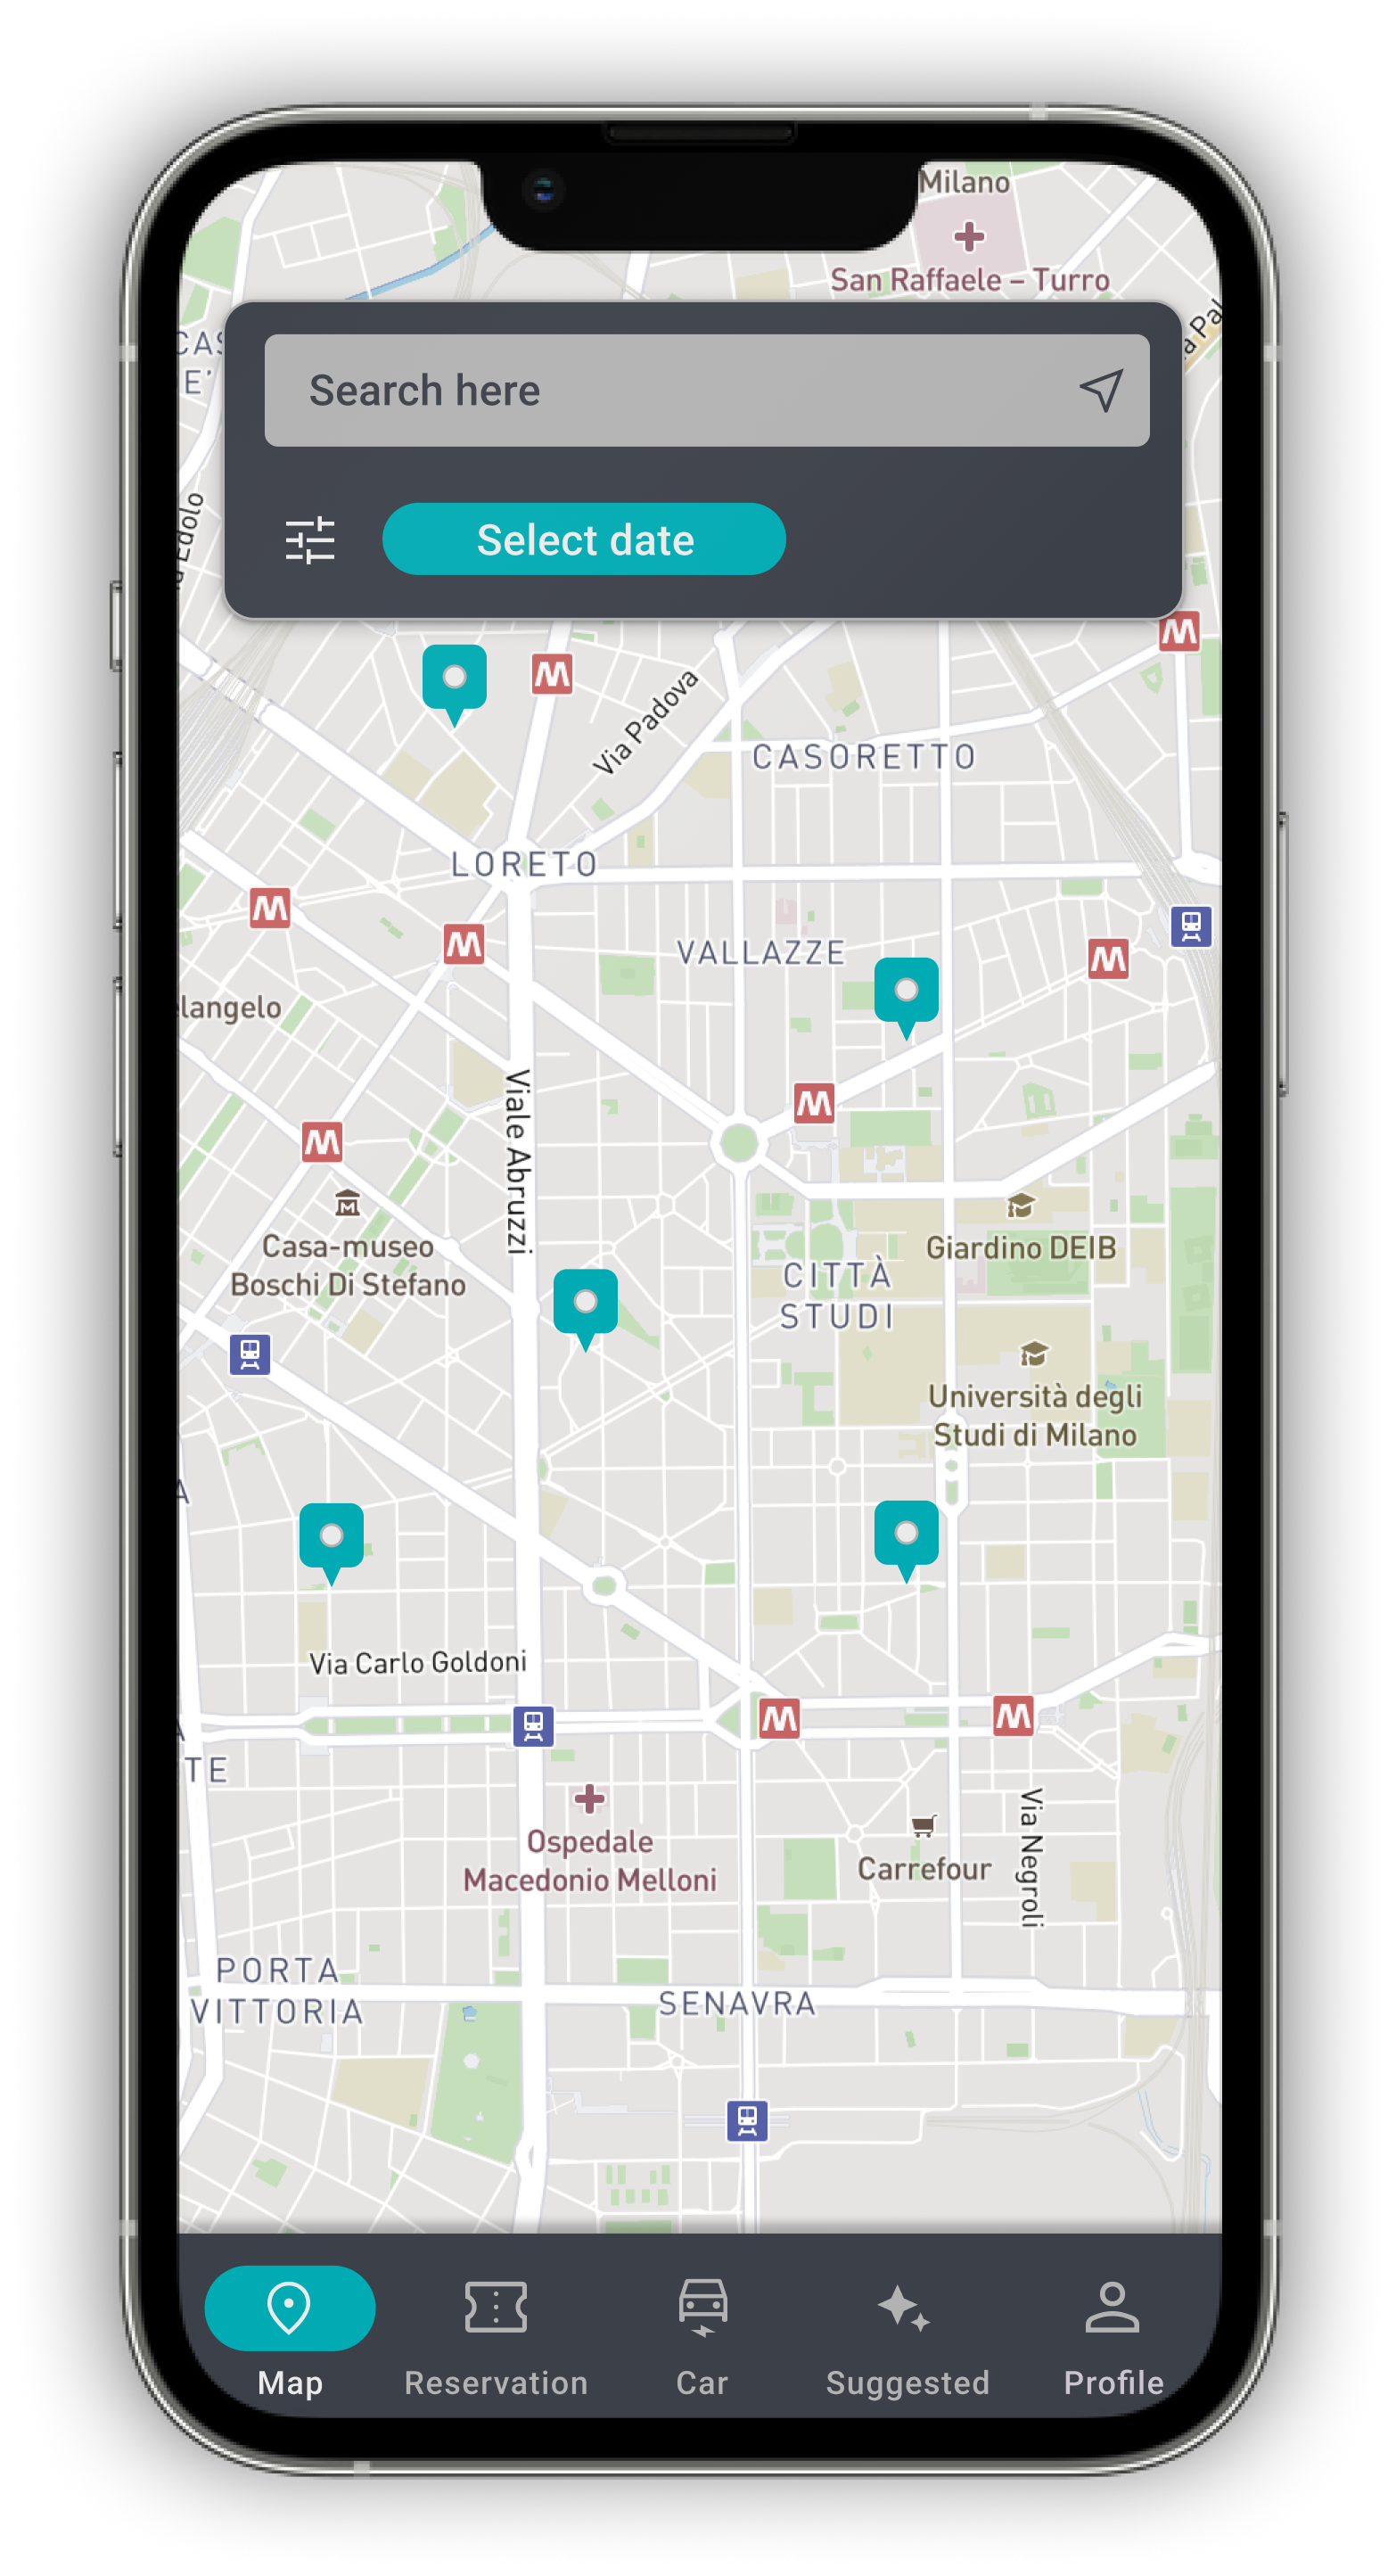
\includegraphics[scale=0.32]{src/mockups/home.png}
    }
    \subfloat[Selected EVCP]{
        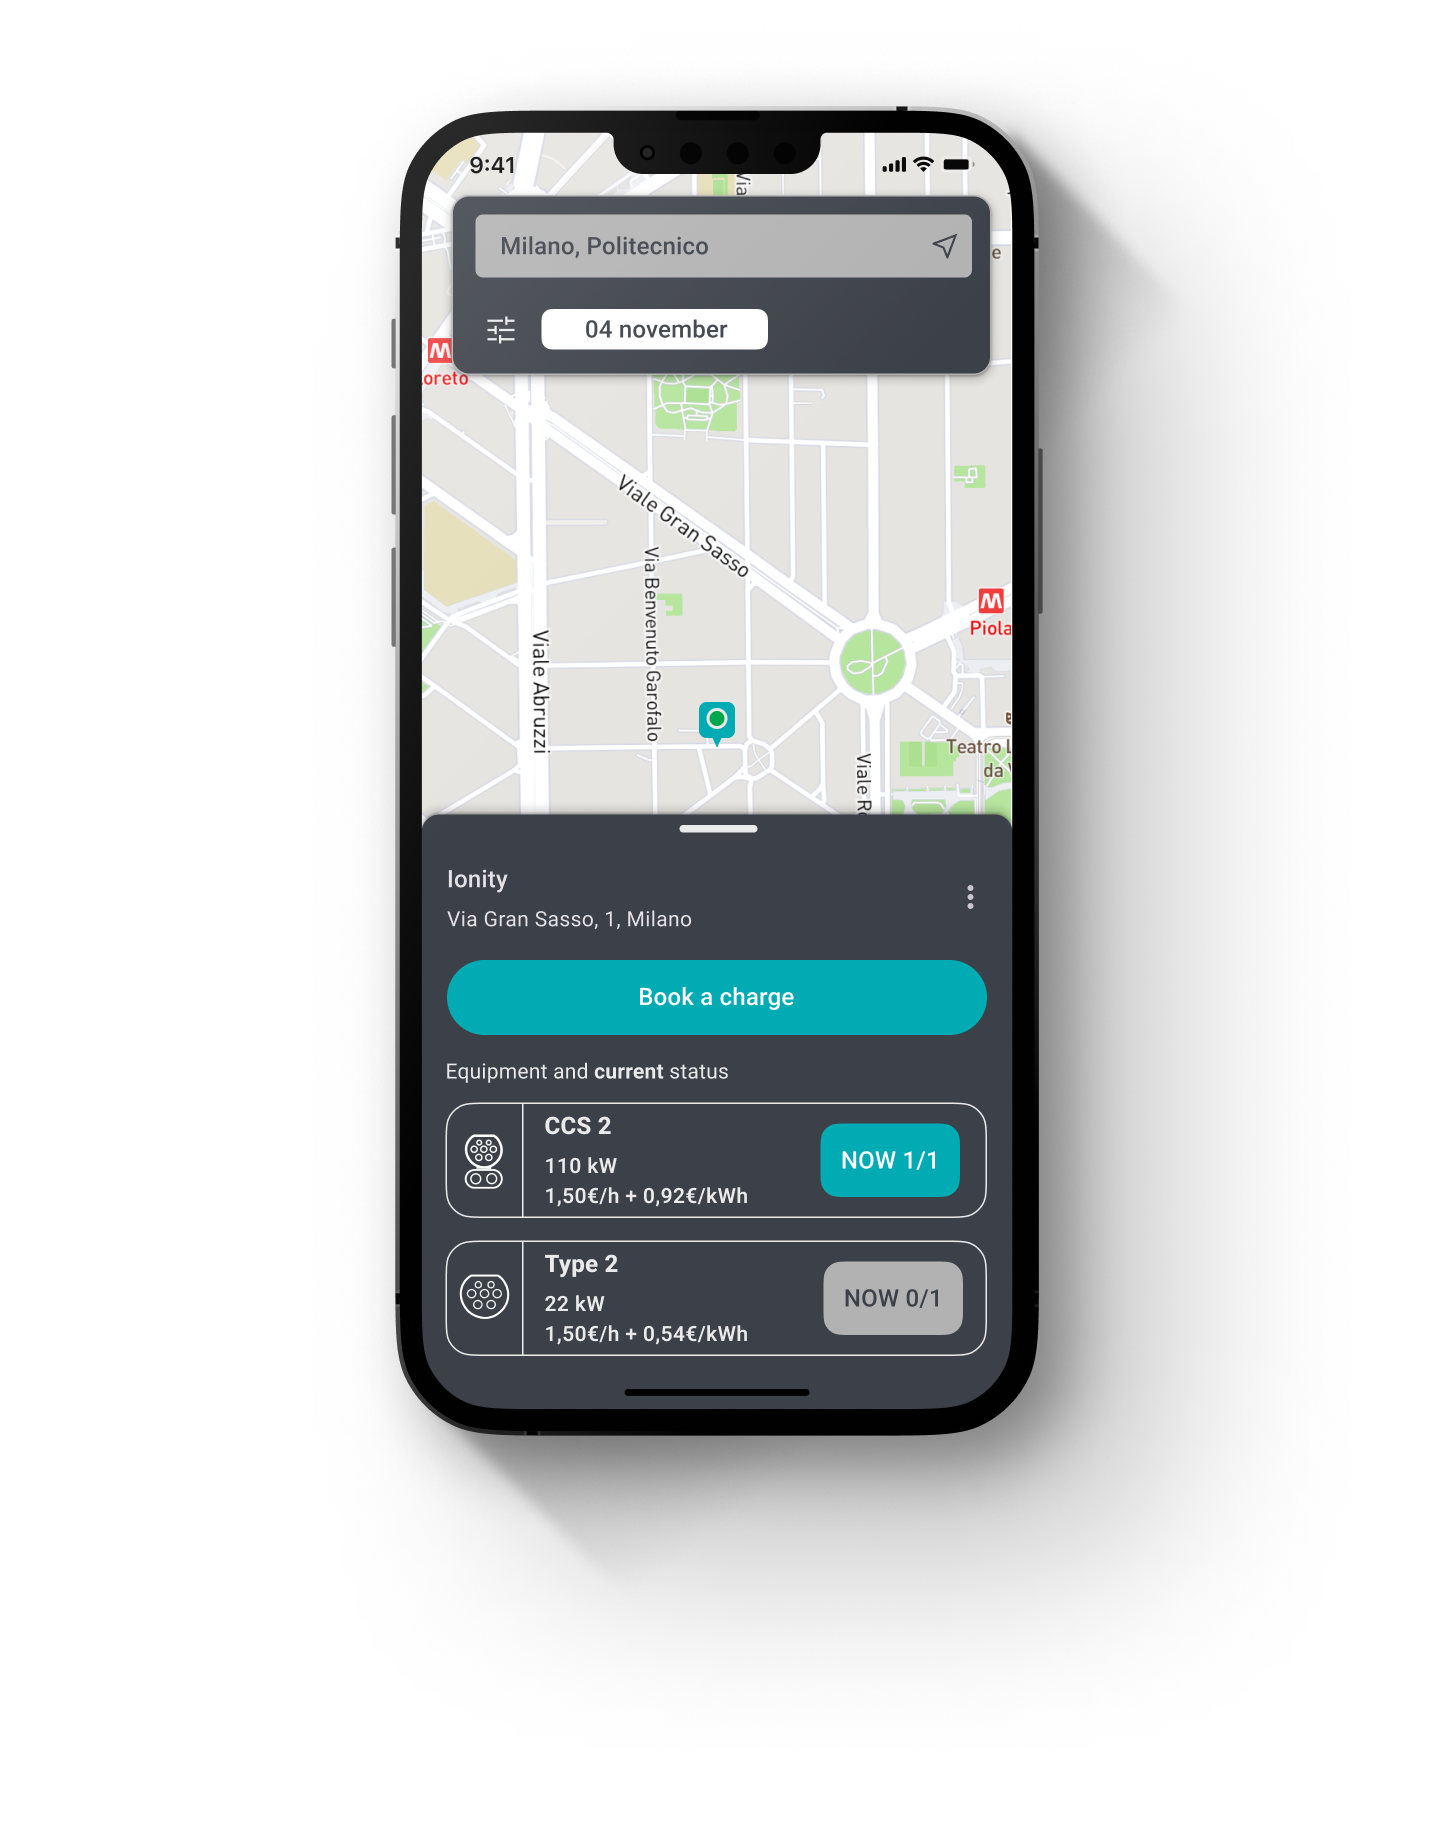
\includegraphics[scale=0.32]{src/mockups/selectedStation.png}
    }
    \newline
    \subfloat[Book charge tab]{
        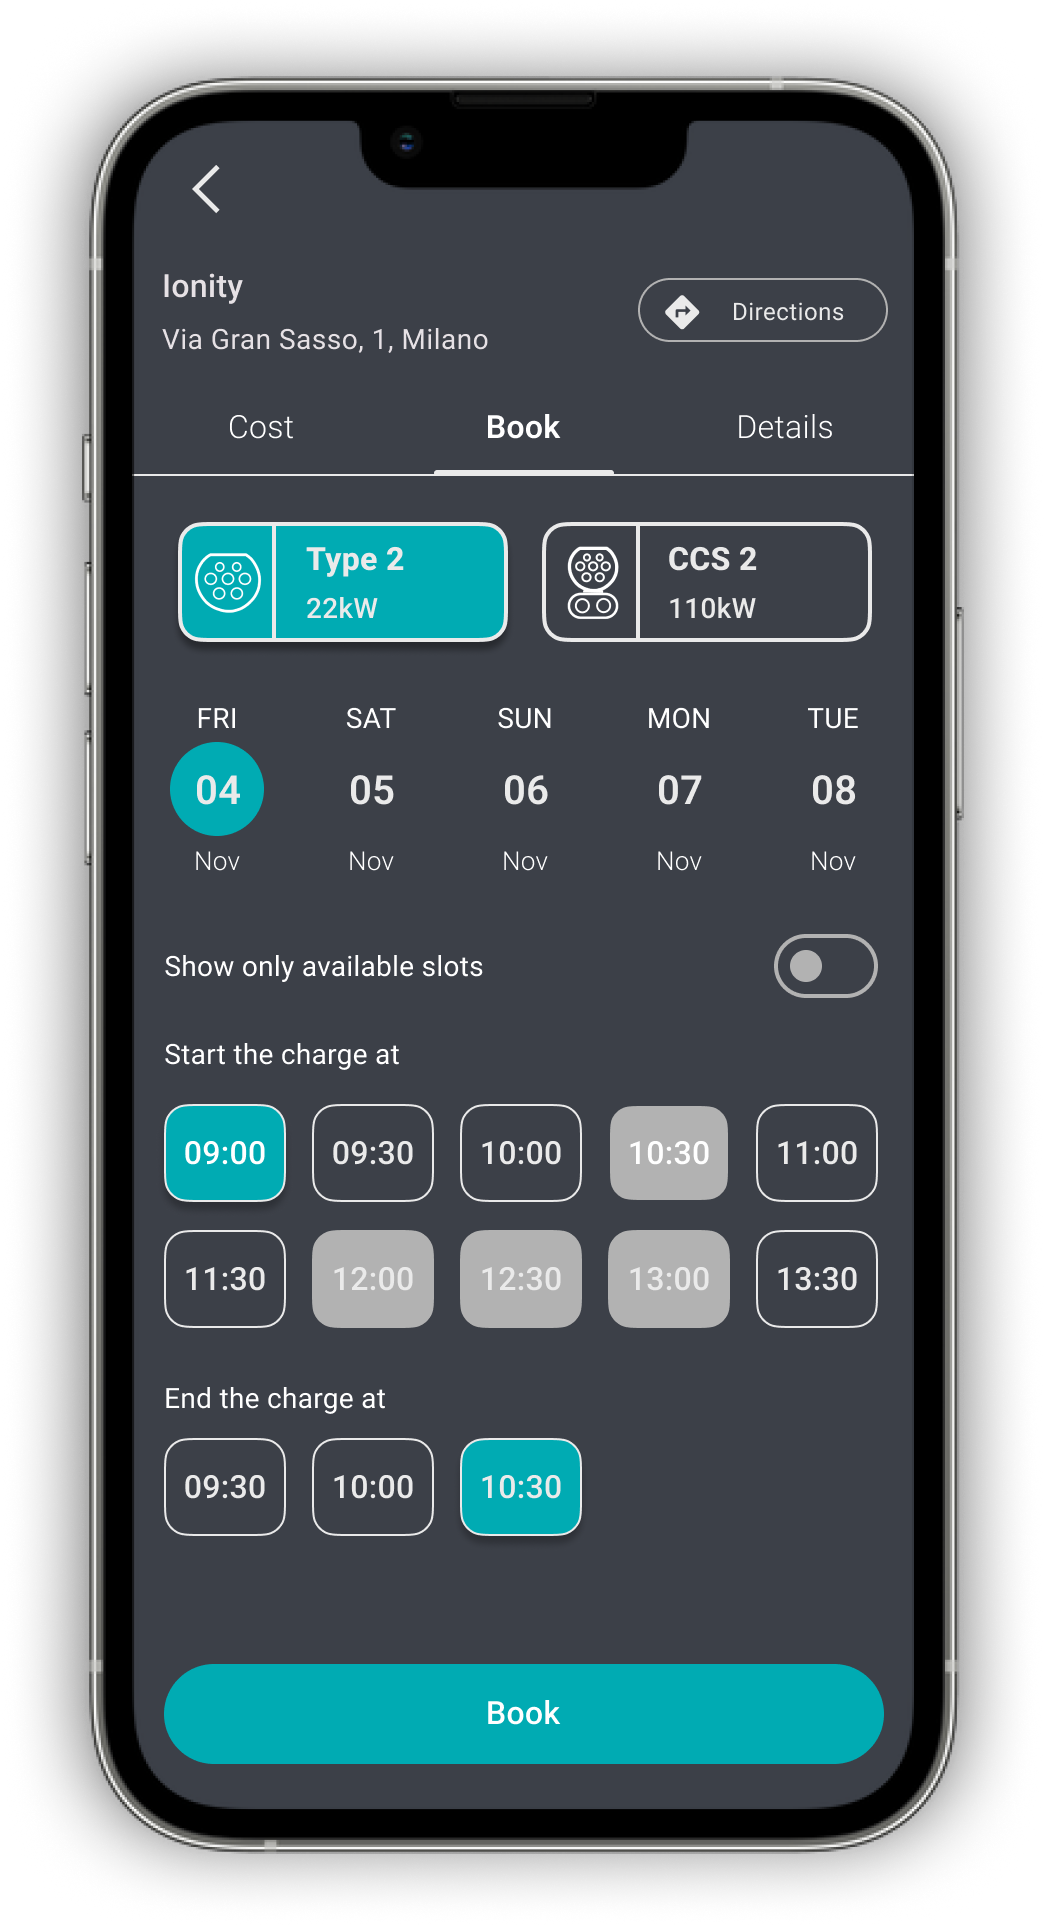
\includegraphics[scale=0.32]{src/mockups/book_charge.png}
    }
    \subfloat[Book cost tab]{
        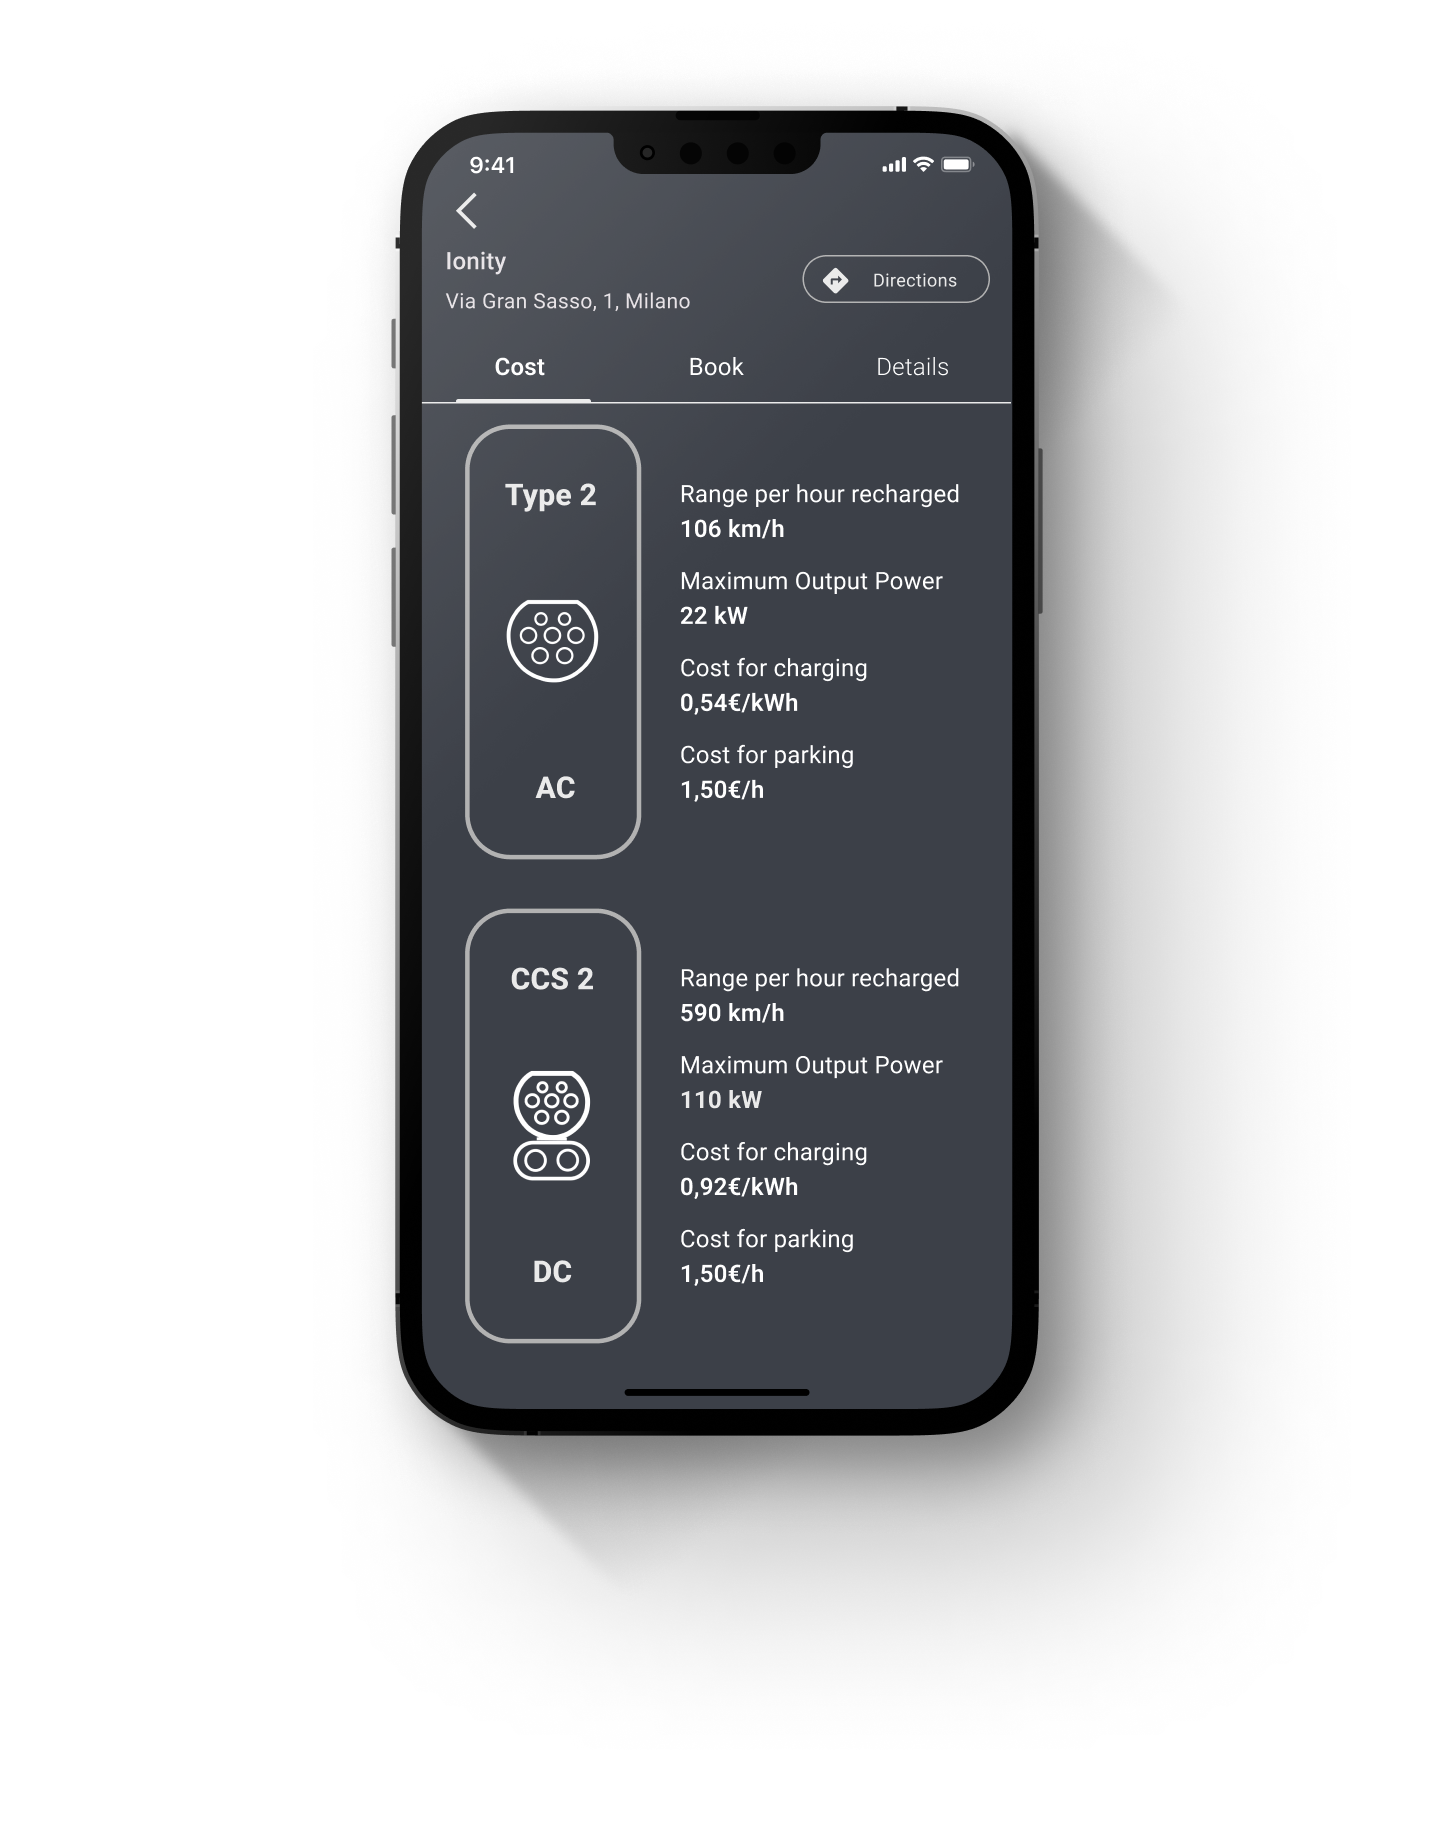
\includegraphics[scale=0.32]{src/mockups/book_cost.png}
    }
    \newline
\end{figure}

\begin{figure}[H]
    \centering
    \subfloat[Car status]{
        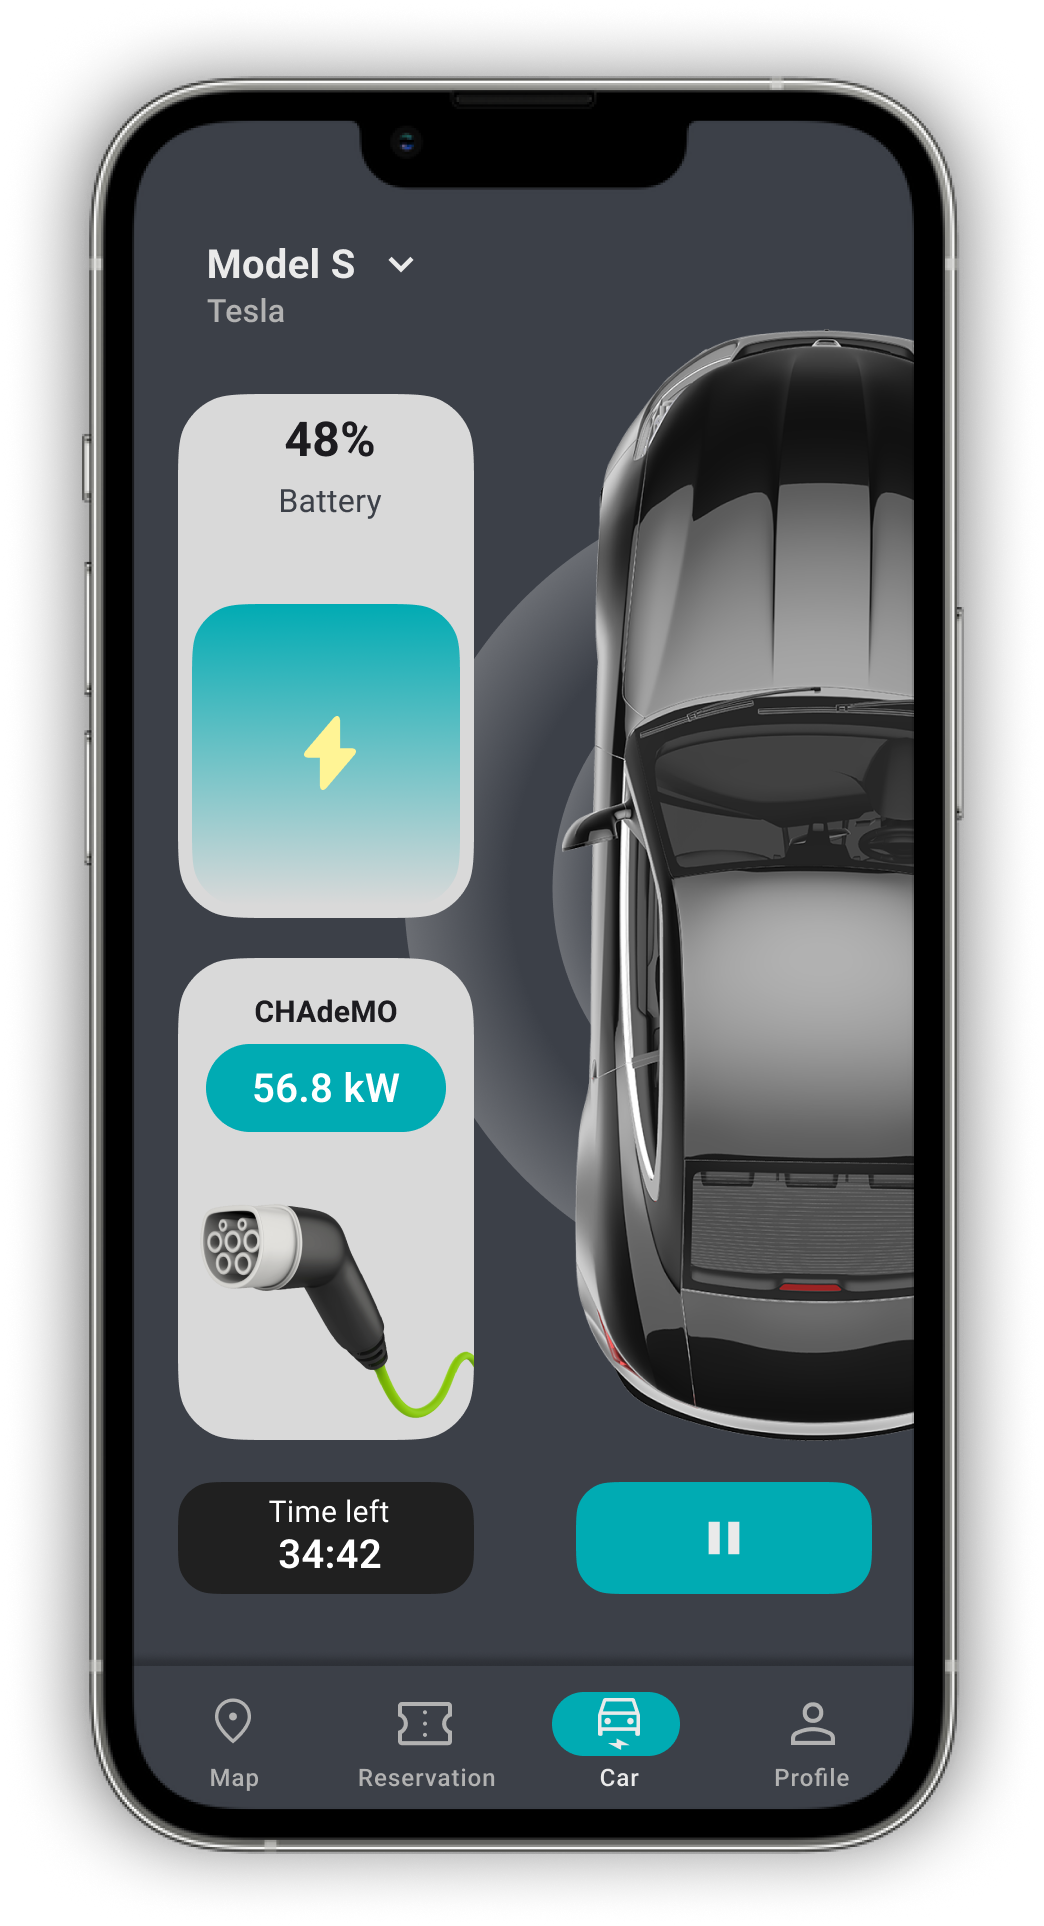
\includegraphics[scale=0.32]{src/mockups/car.png}
    }
    \subfloat[Add a car]{
        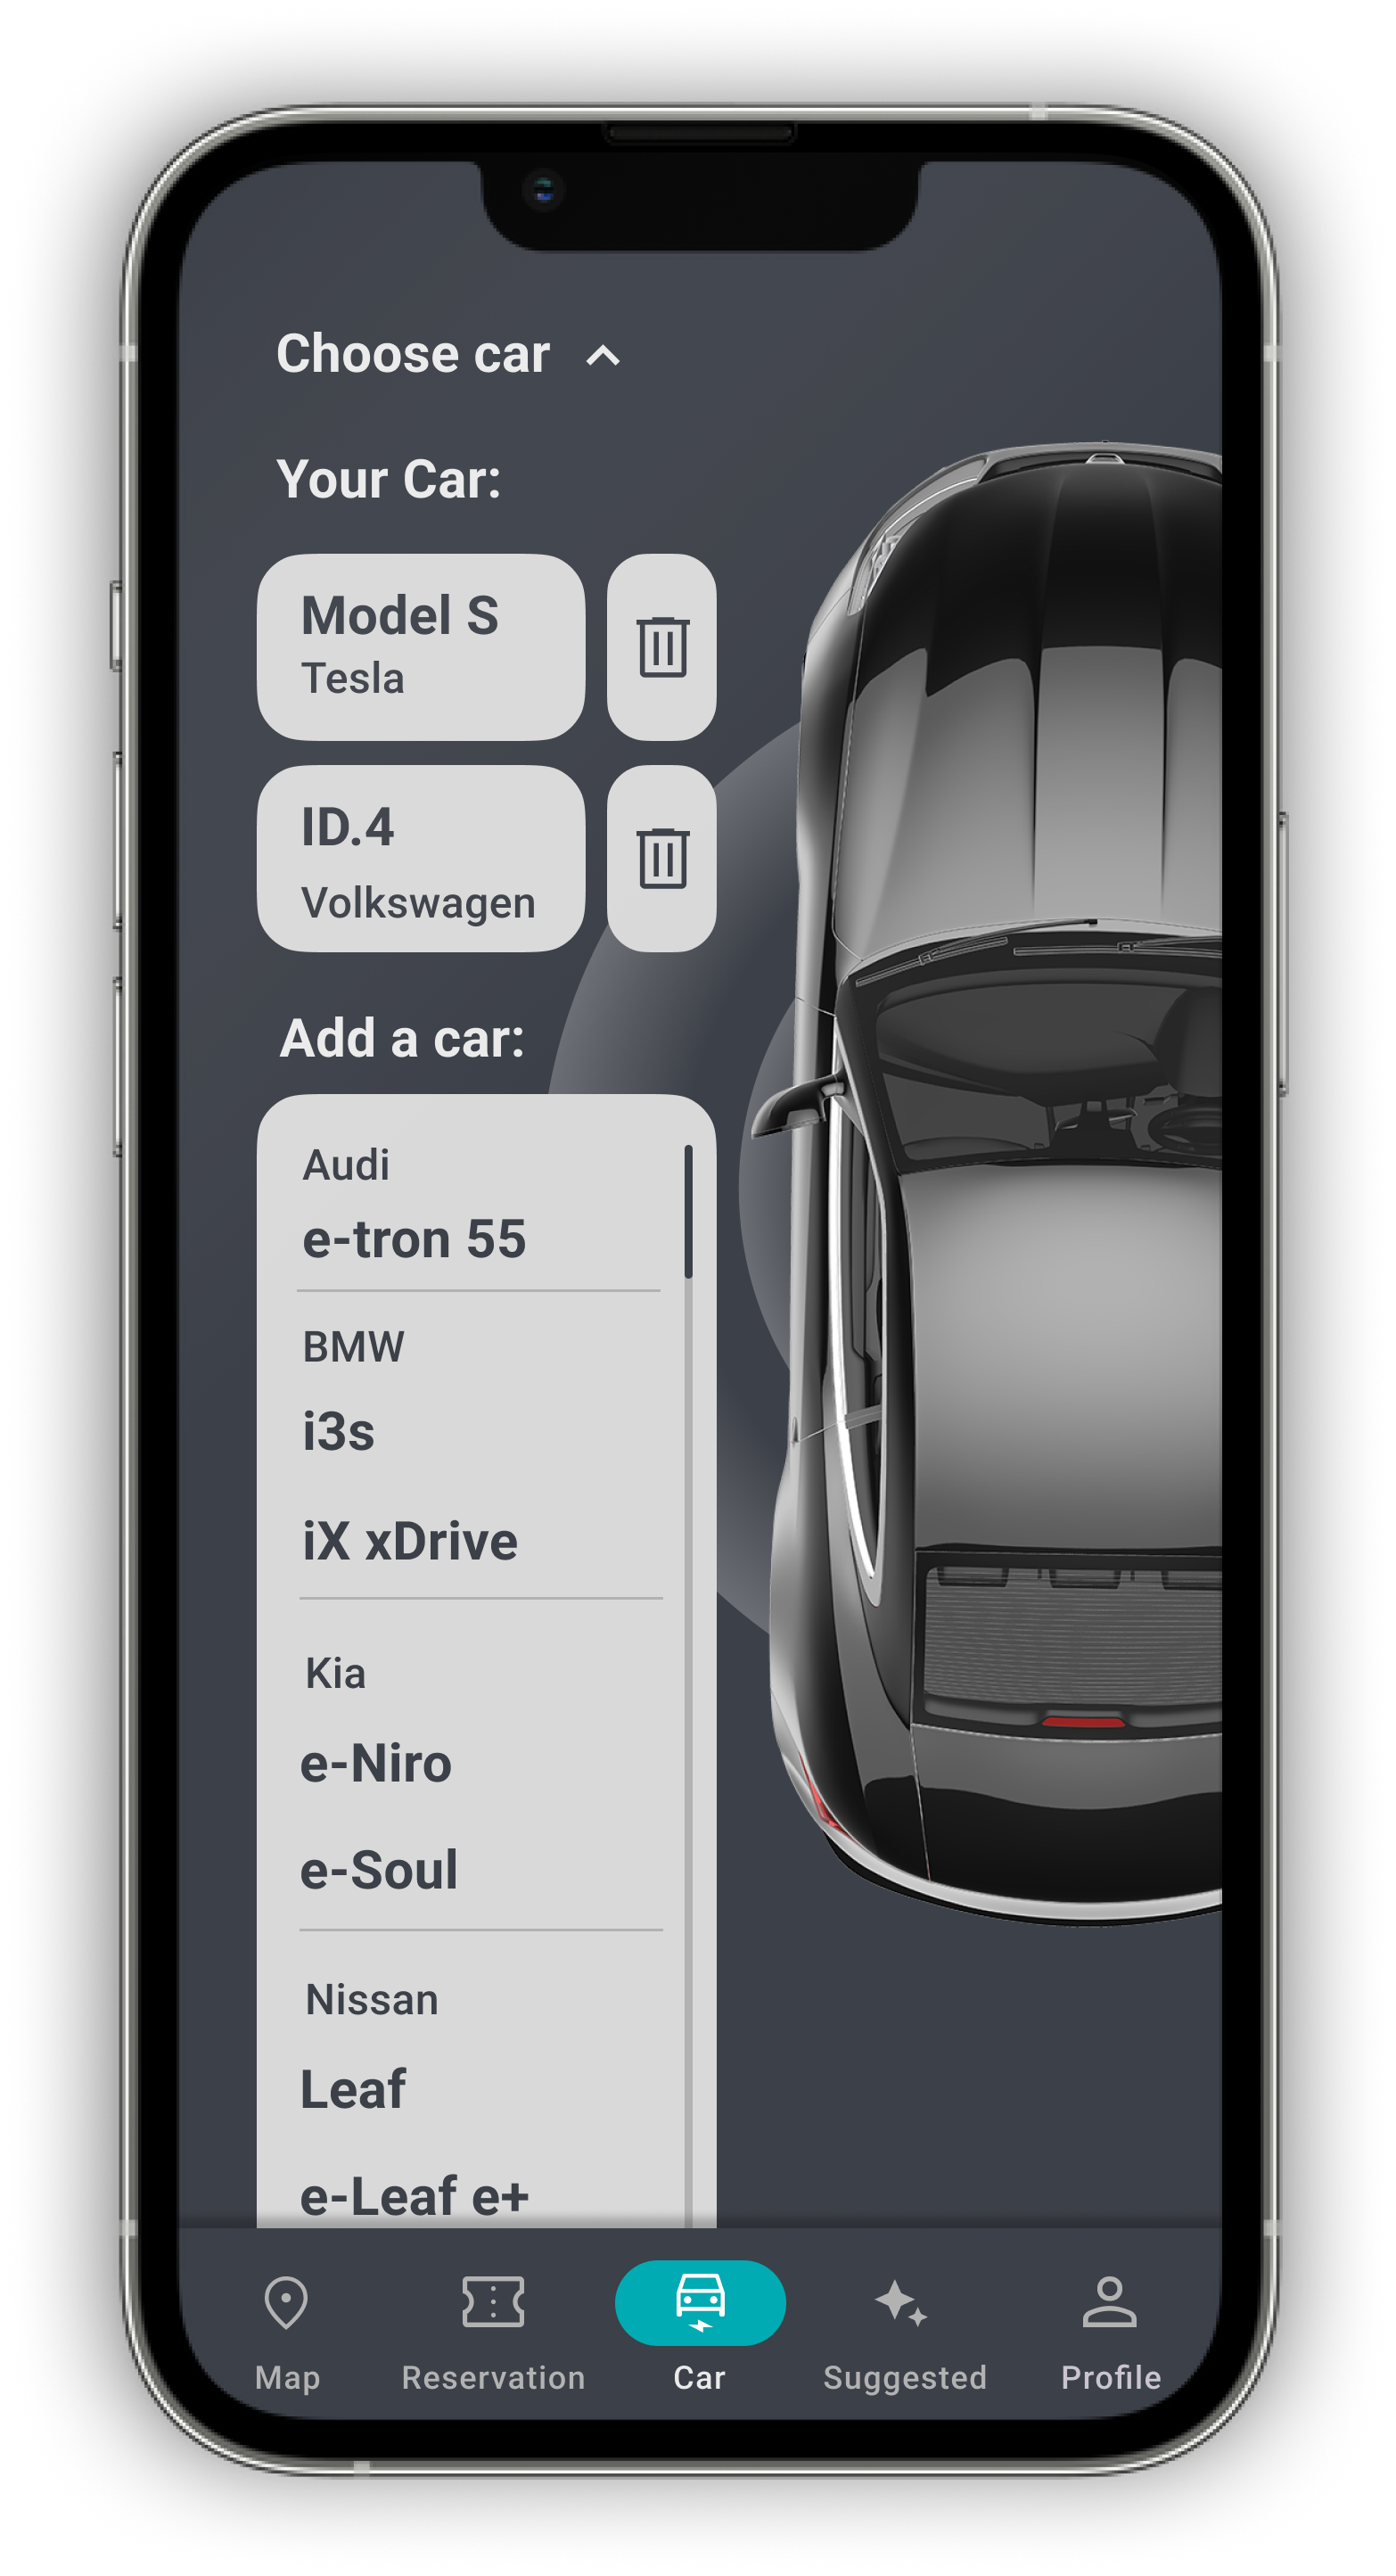
\includegraphics[scale=0.32]{src/mockups/car_add.png}
    }
    \newline
    \subfloat[Reservations]{
        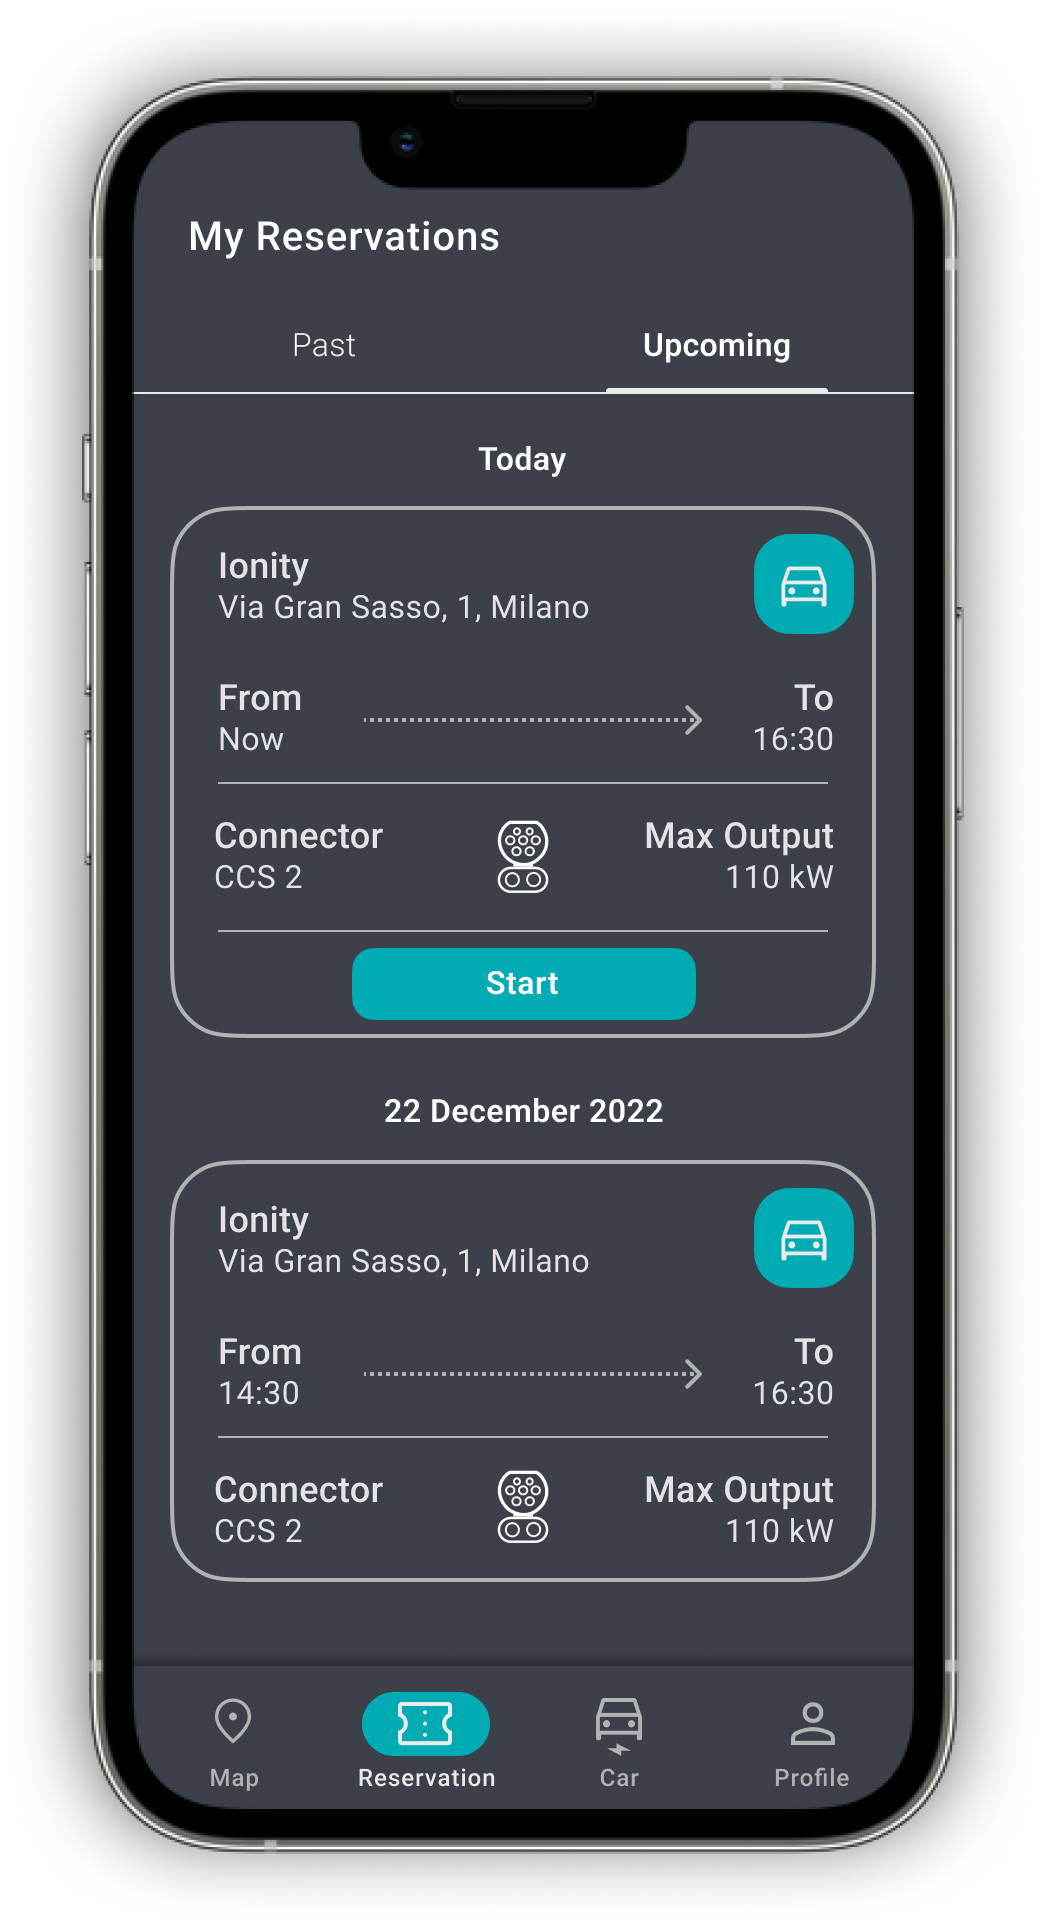
\includegraphics[scale=0.32]{src/mockups/reservations.png}
    }
    \subfloat[Profile]{
        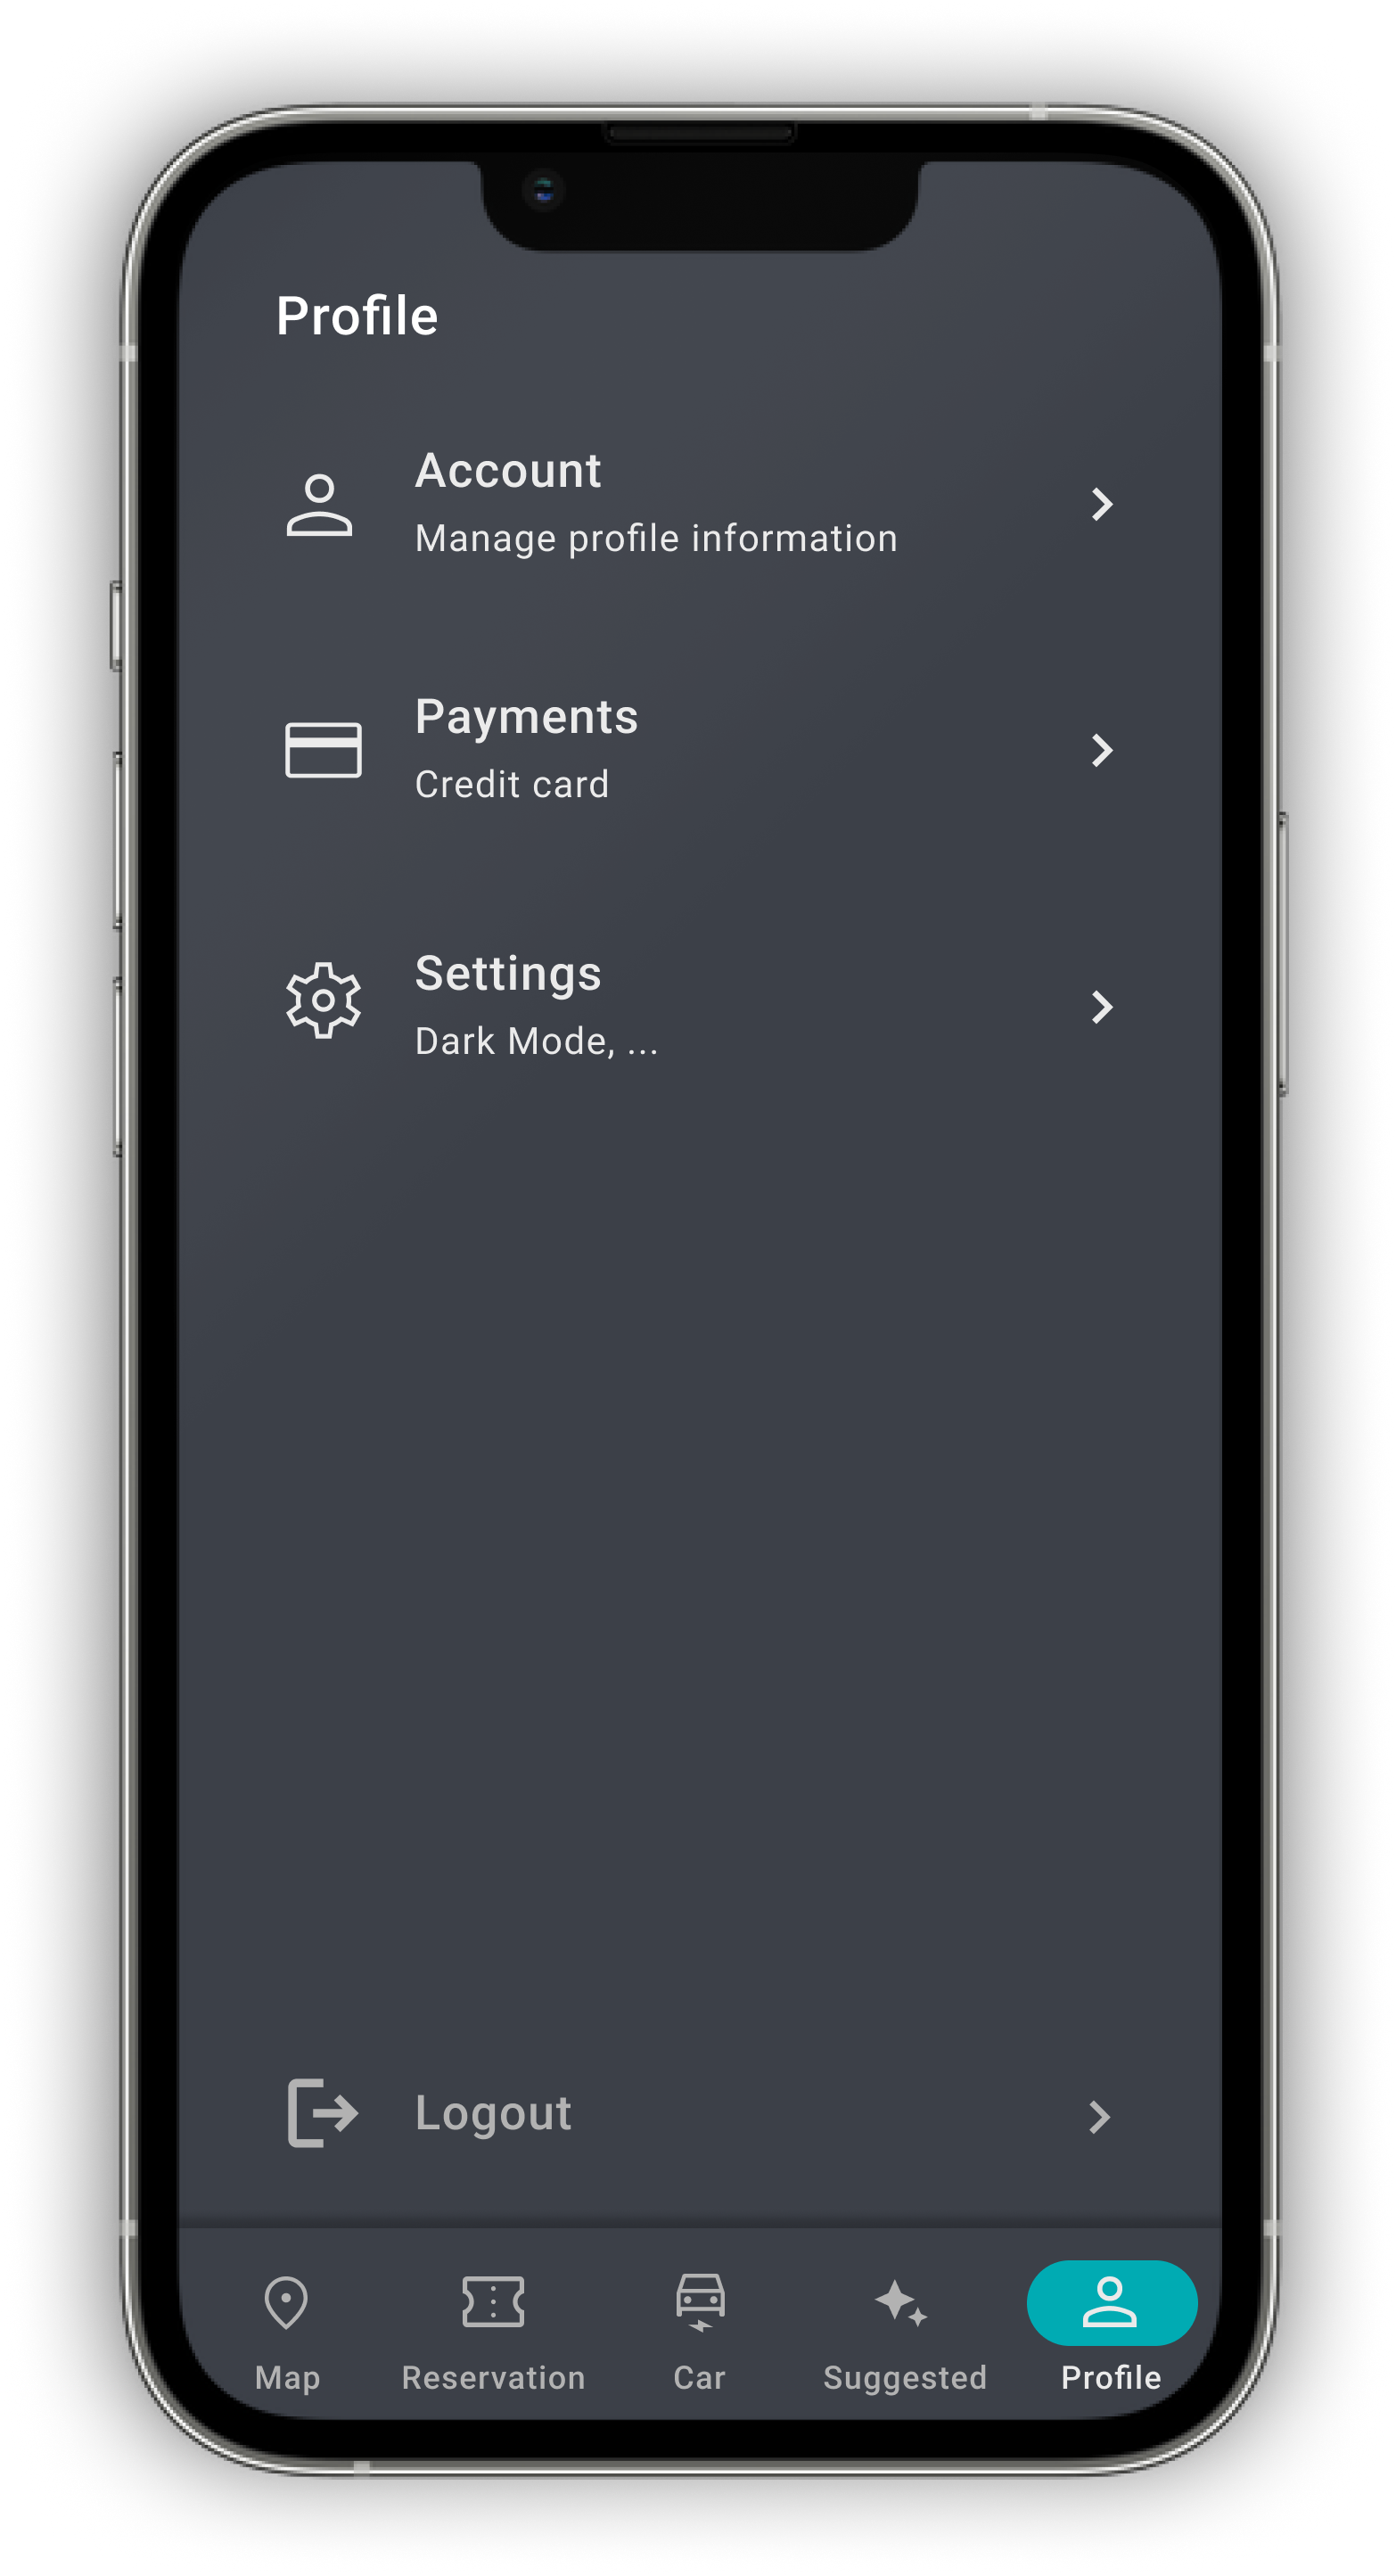
\includegraphics[scale=0.32]{src/mockups/profile.png}
    }
    \newline
    % following mockups
\end{figure}

\begin{figure}[H]
    \centering
    \subfloat[Dashboard]{
        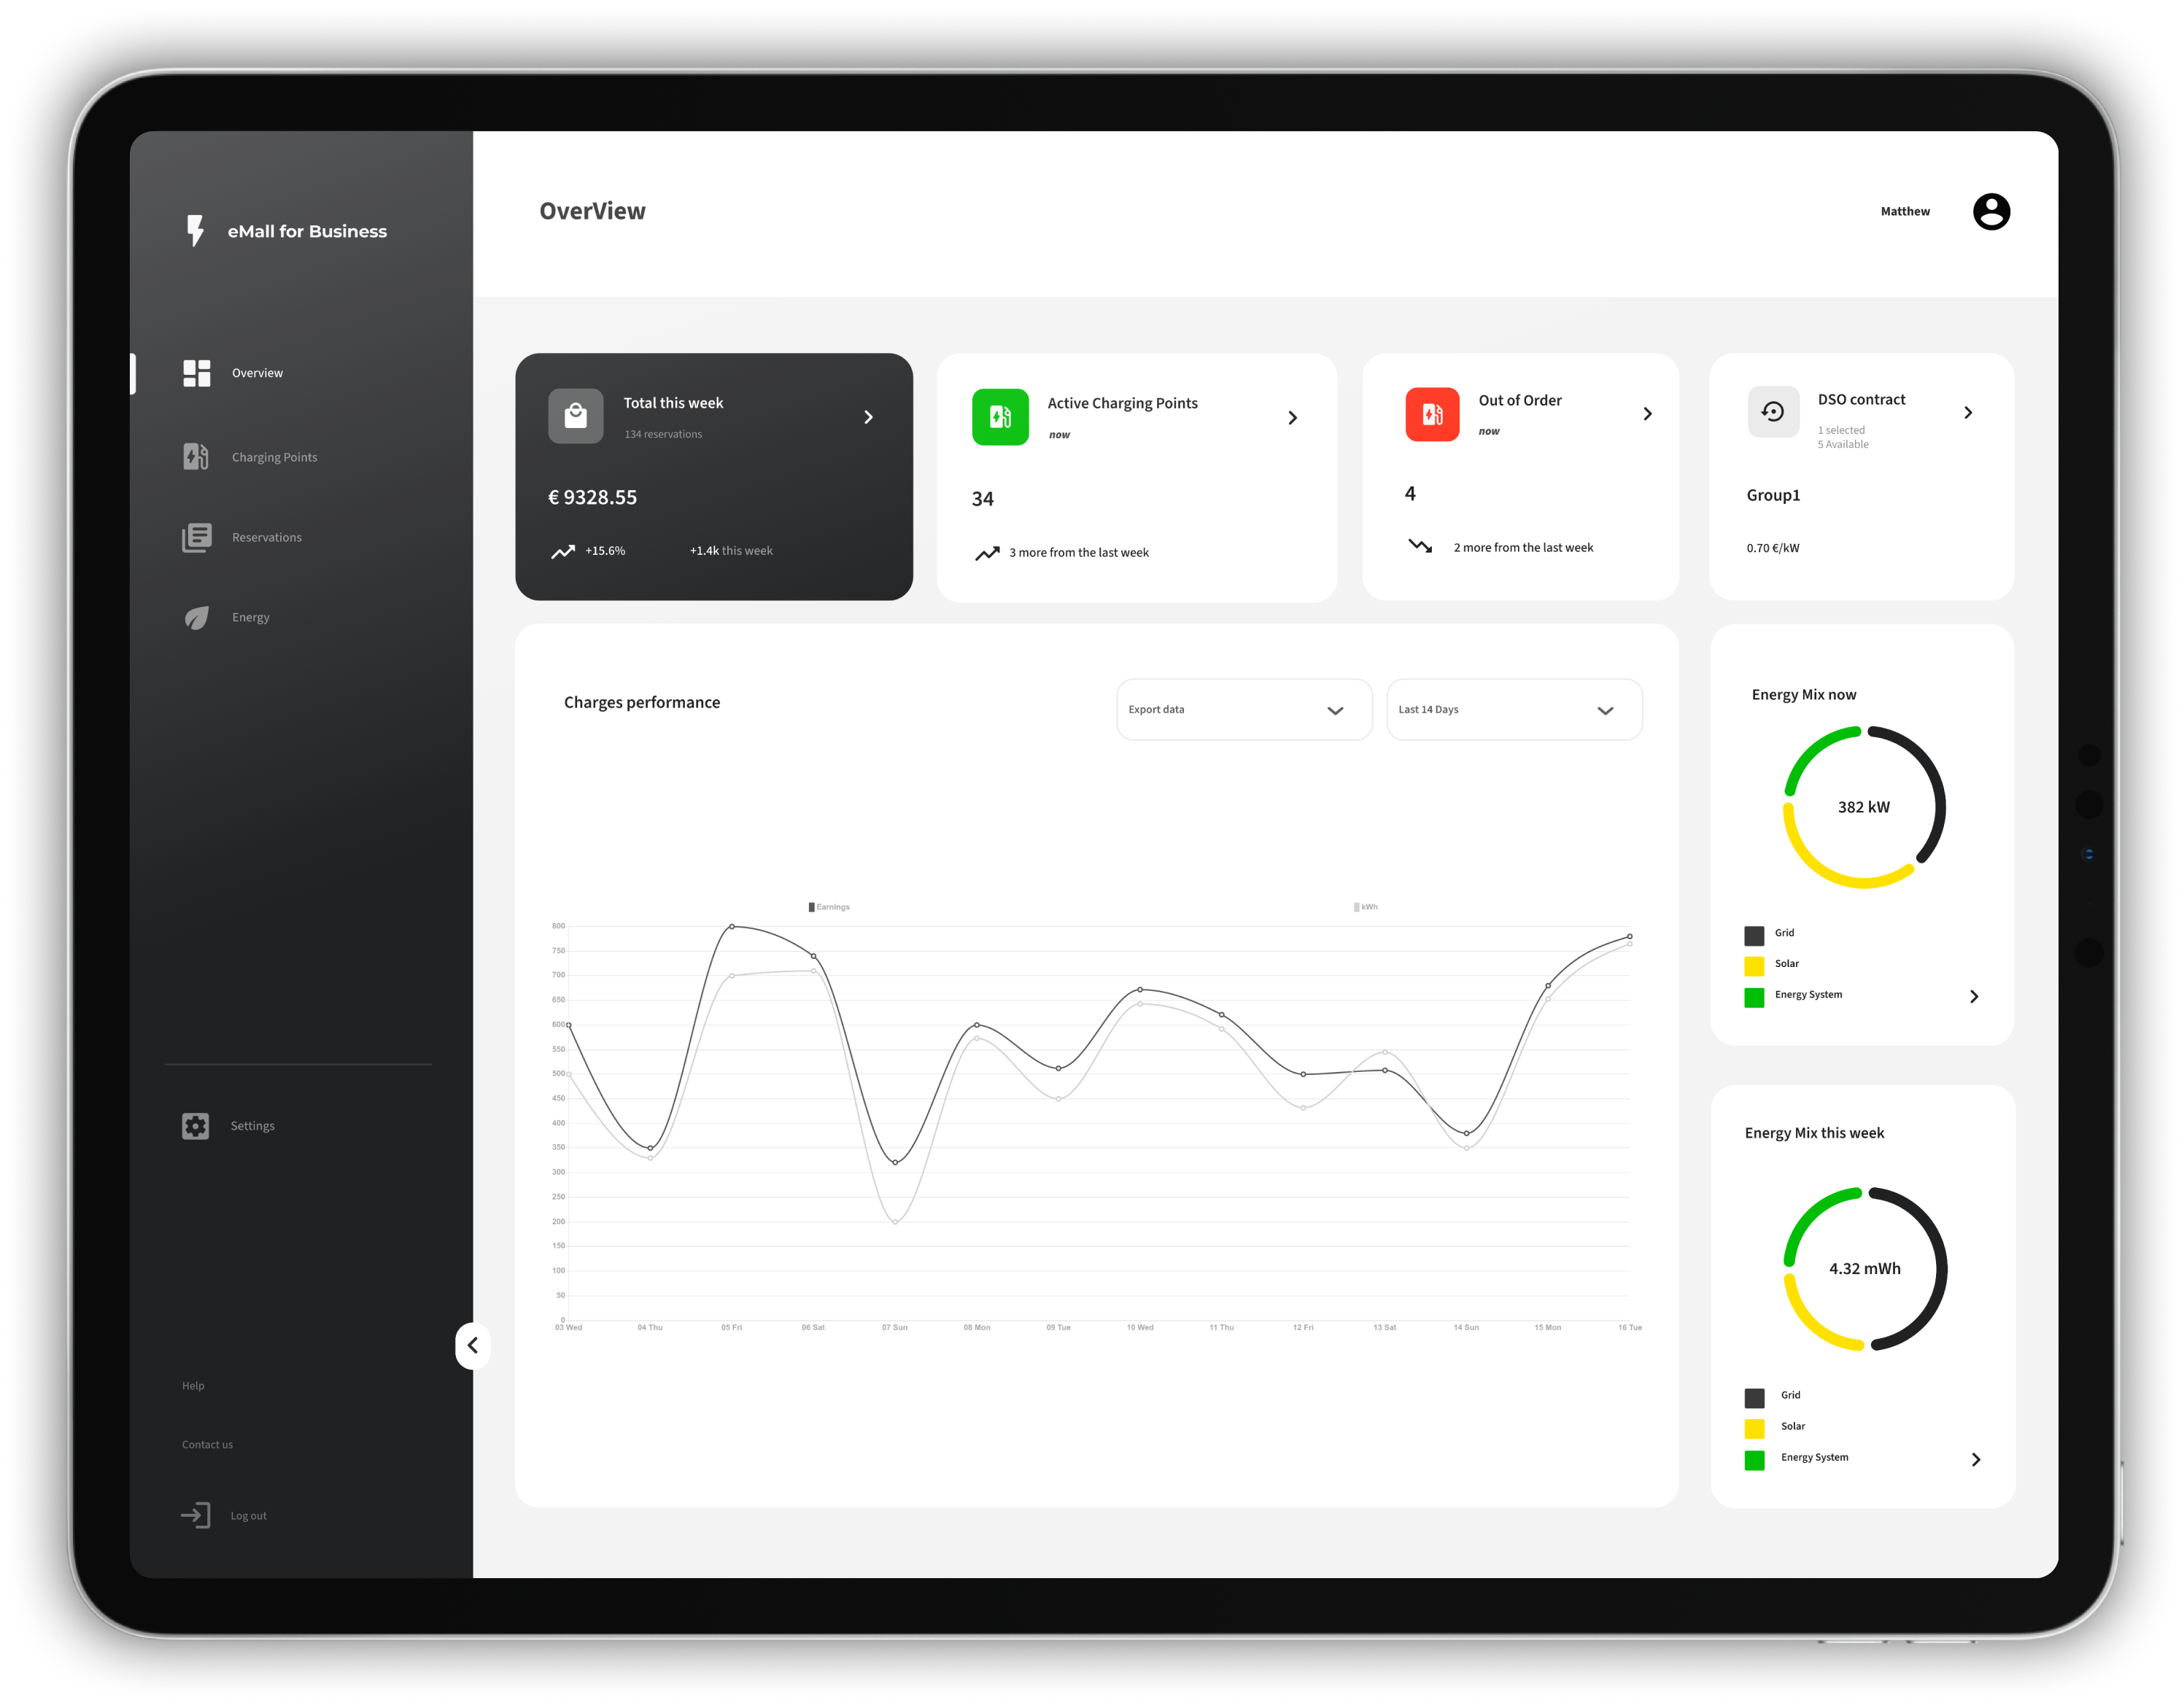
\includegraphics[scale=0.28]{src/mockups/business_dashboard.png}
    }
    \newline
    \subfloat[Charging Points]{
        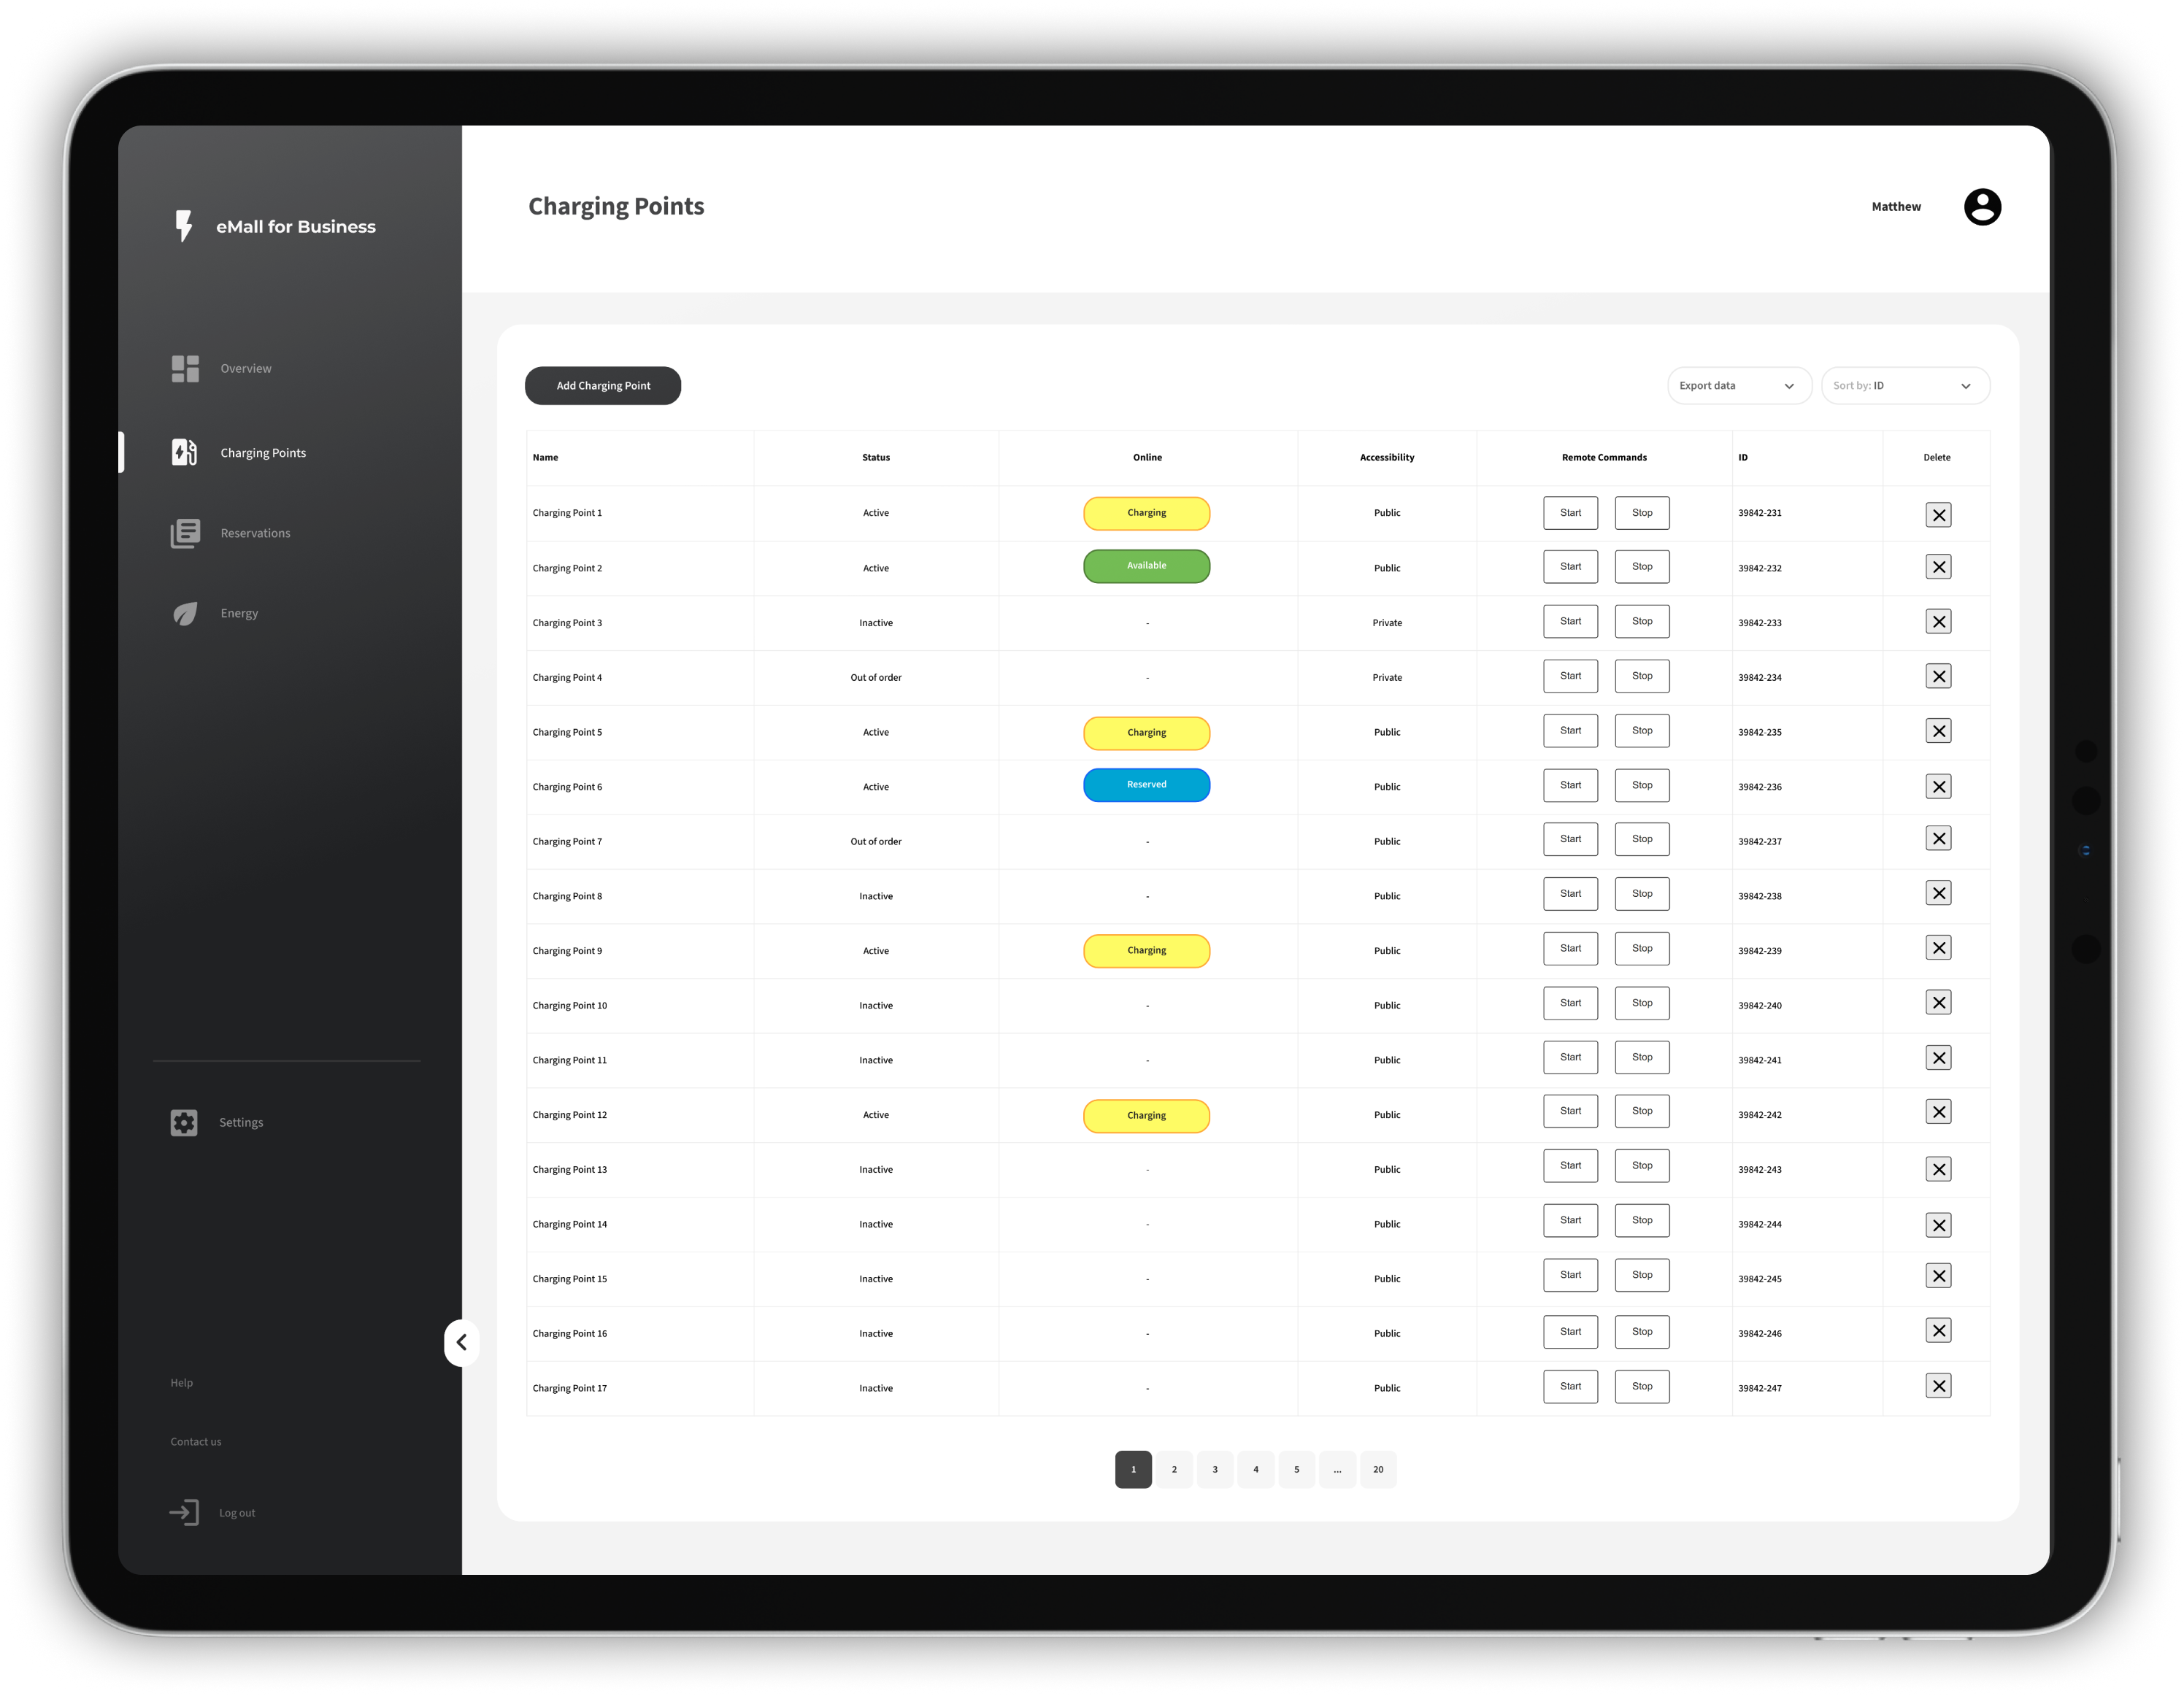
\includegraphics[scale=0.28]{src/mockups/business_CPs.png}
    }
    \newline
\end{figure}

\begin{figure}[H]
    \centering
    \subfloat[Add a Charging Point]{
        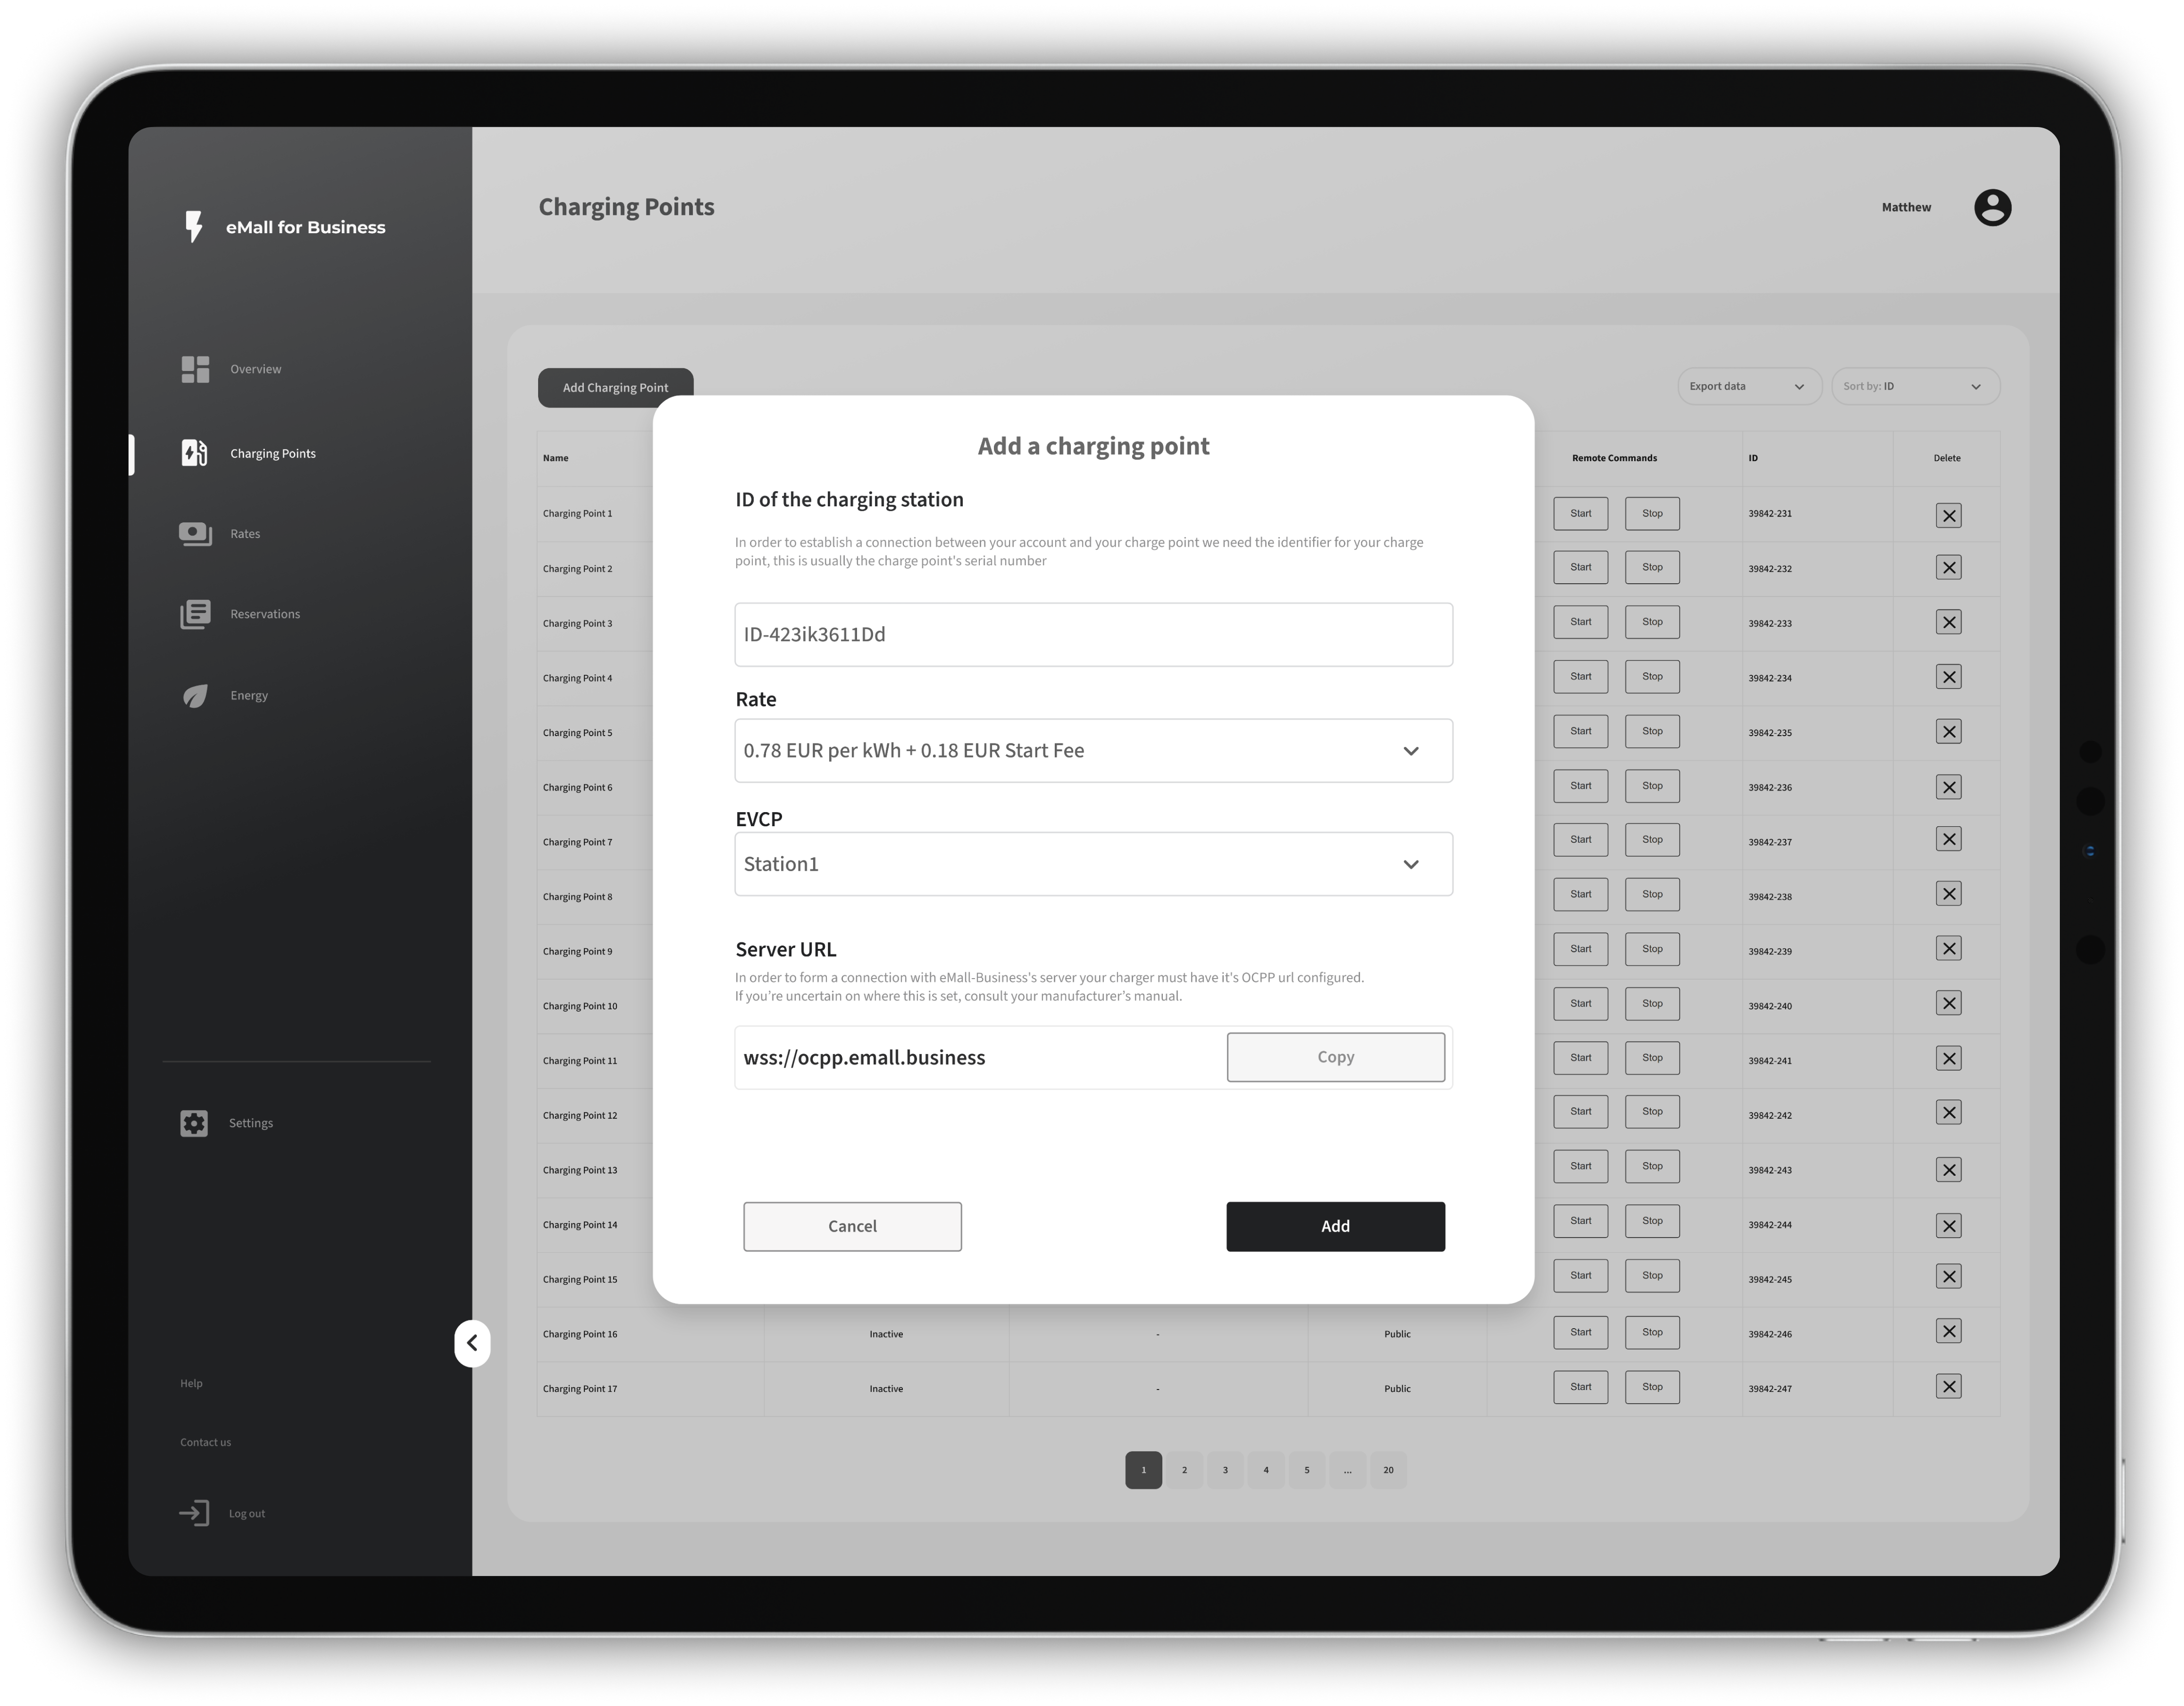
\includegraphics[scale=0.28]{src/mockups/business_addCP.png}
    }
    \newline
    \subfloat[Charging Point]{
        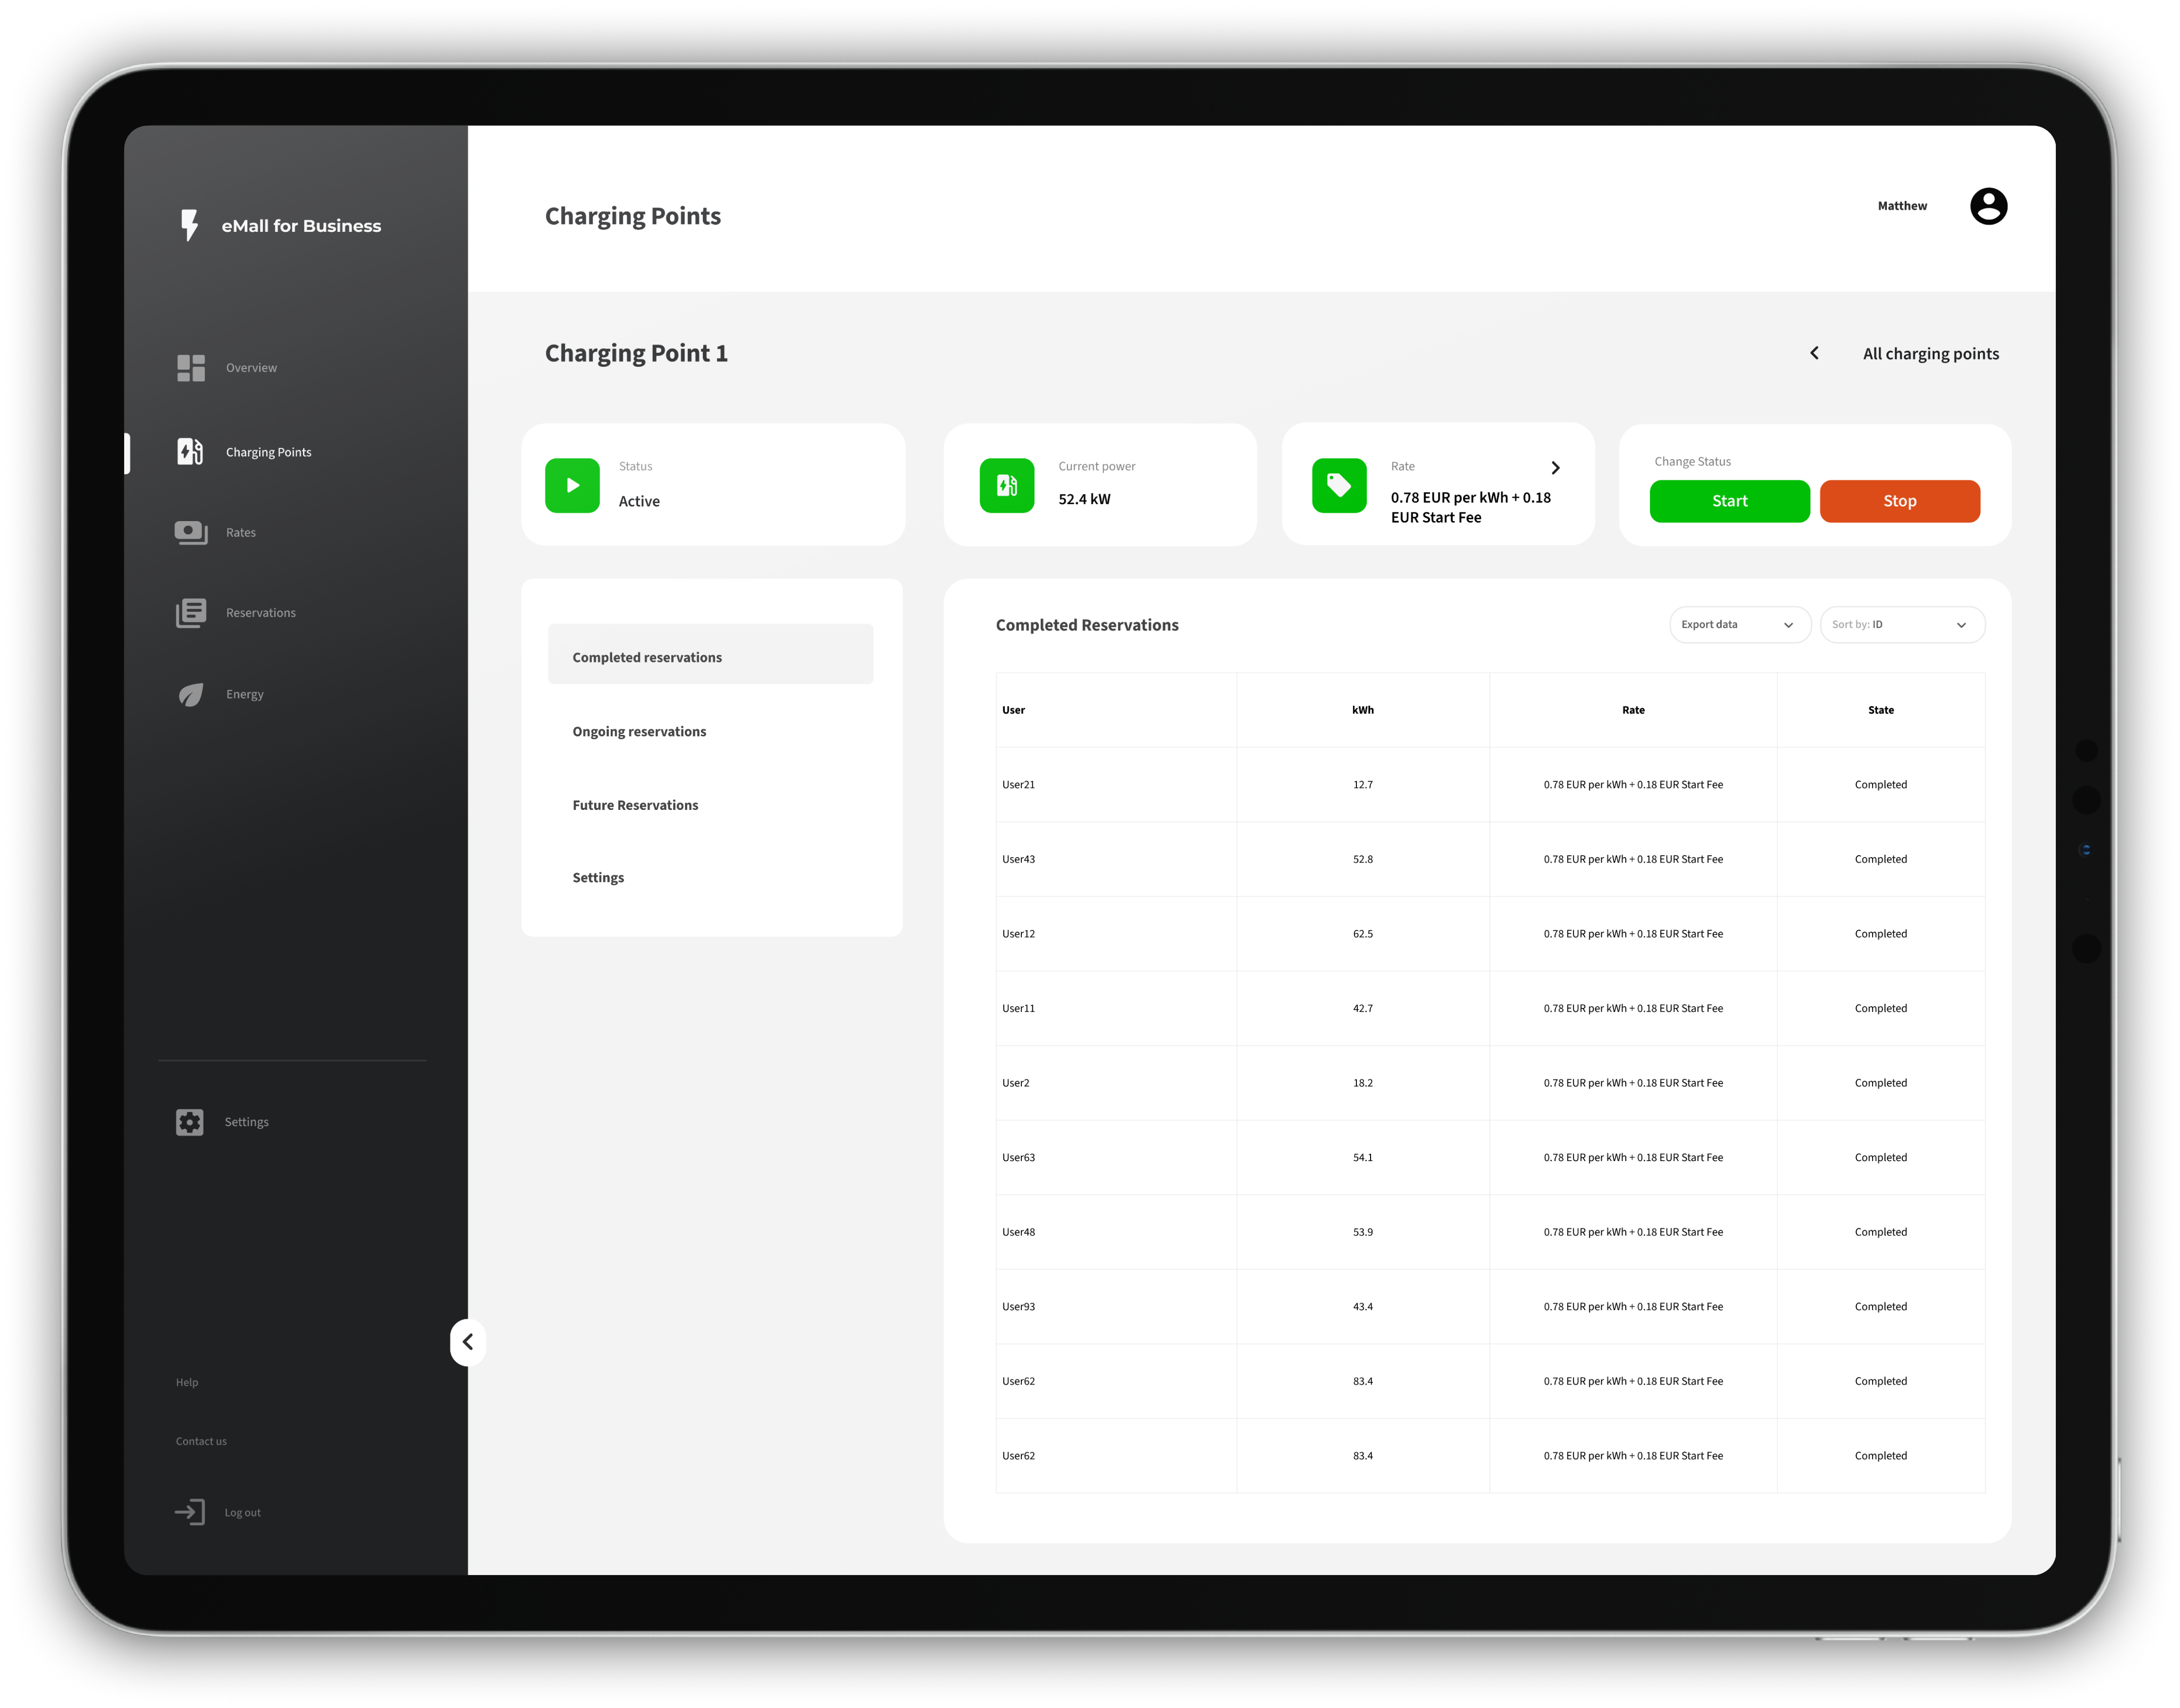
\includegraphics[scale=0.28]{src/mockups/business_CP.png}
    }
    \newline
\end{figure}

\begin{figure}[H]
    \centering
    \subfloat[Reservations list]{
        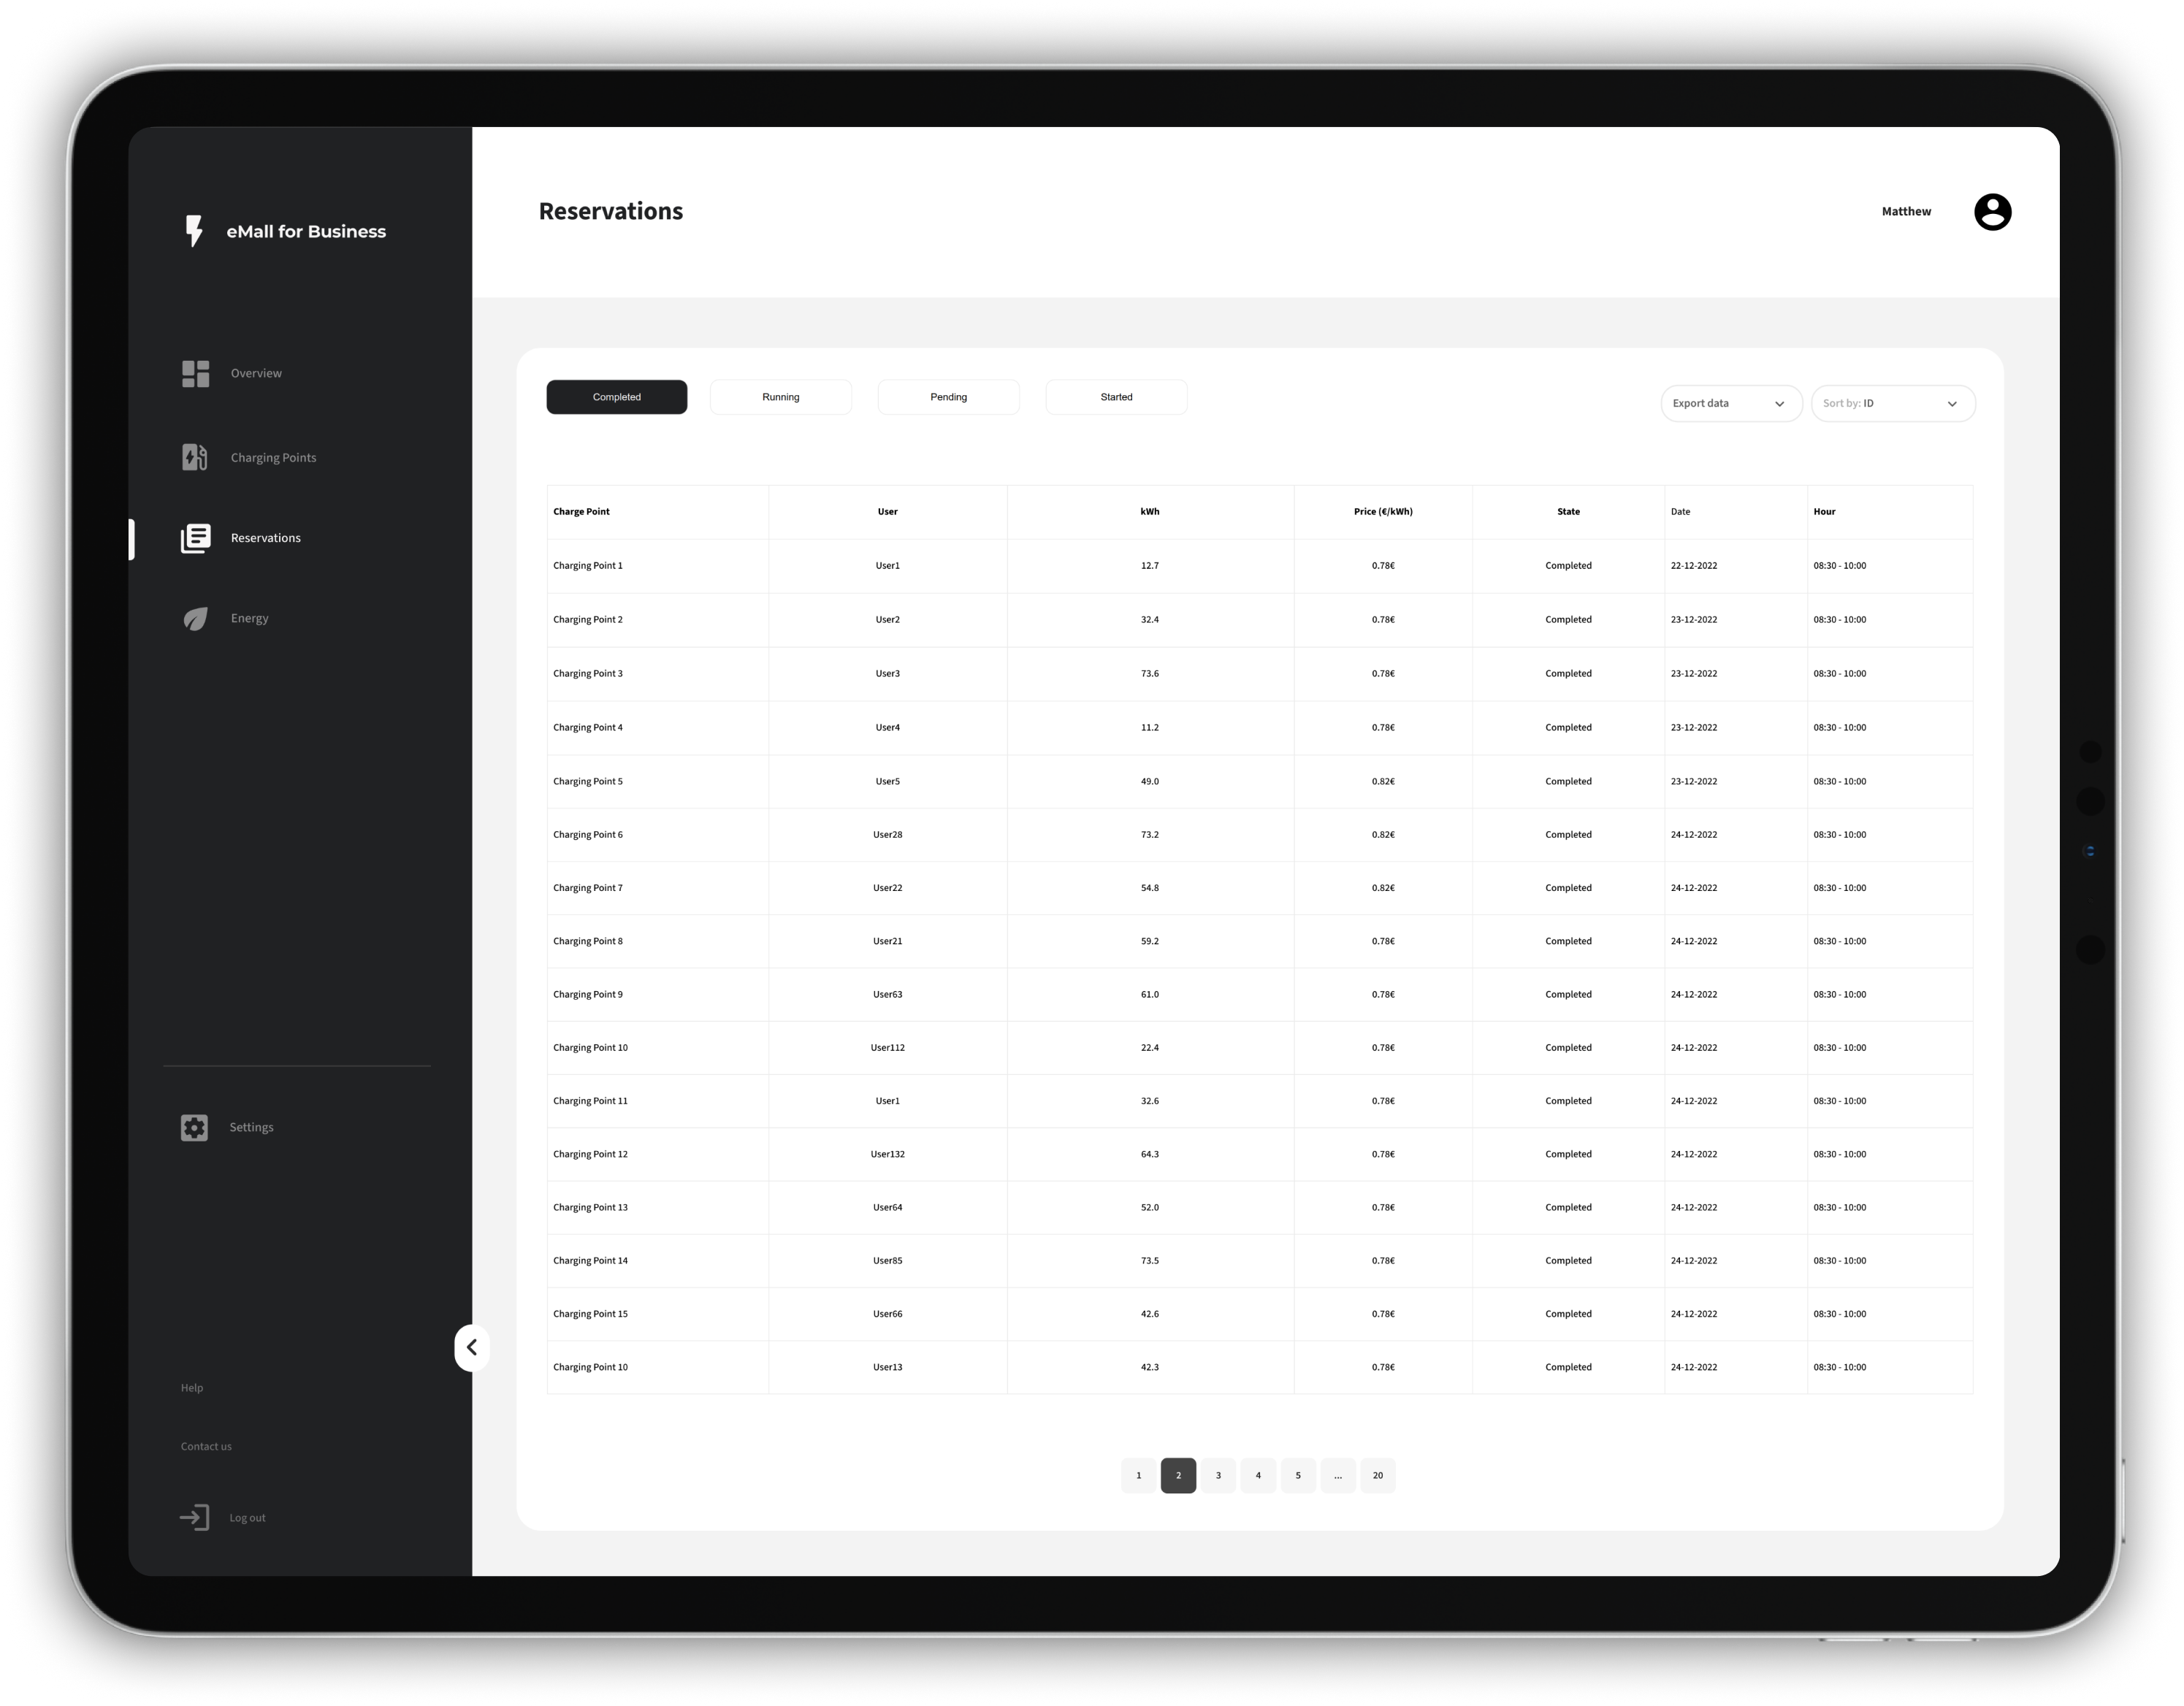
\includegraphics[scale=0.28]{src/mockups/business_reservations.png}
    }
    \newline
    \subfloat[Energy management]{
        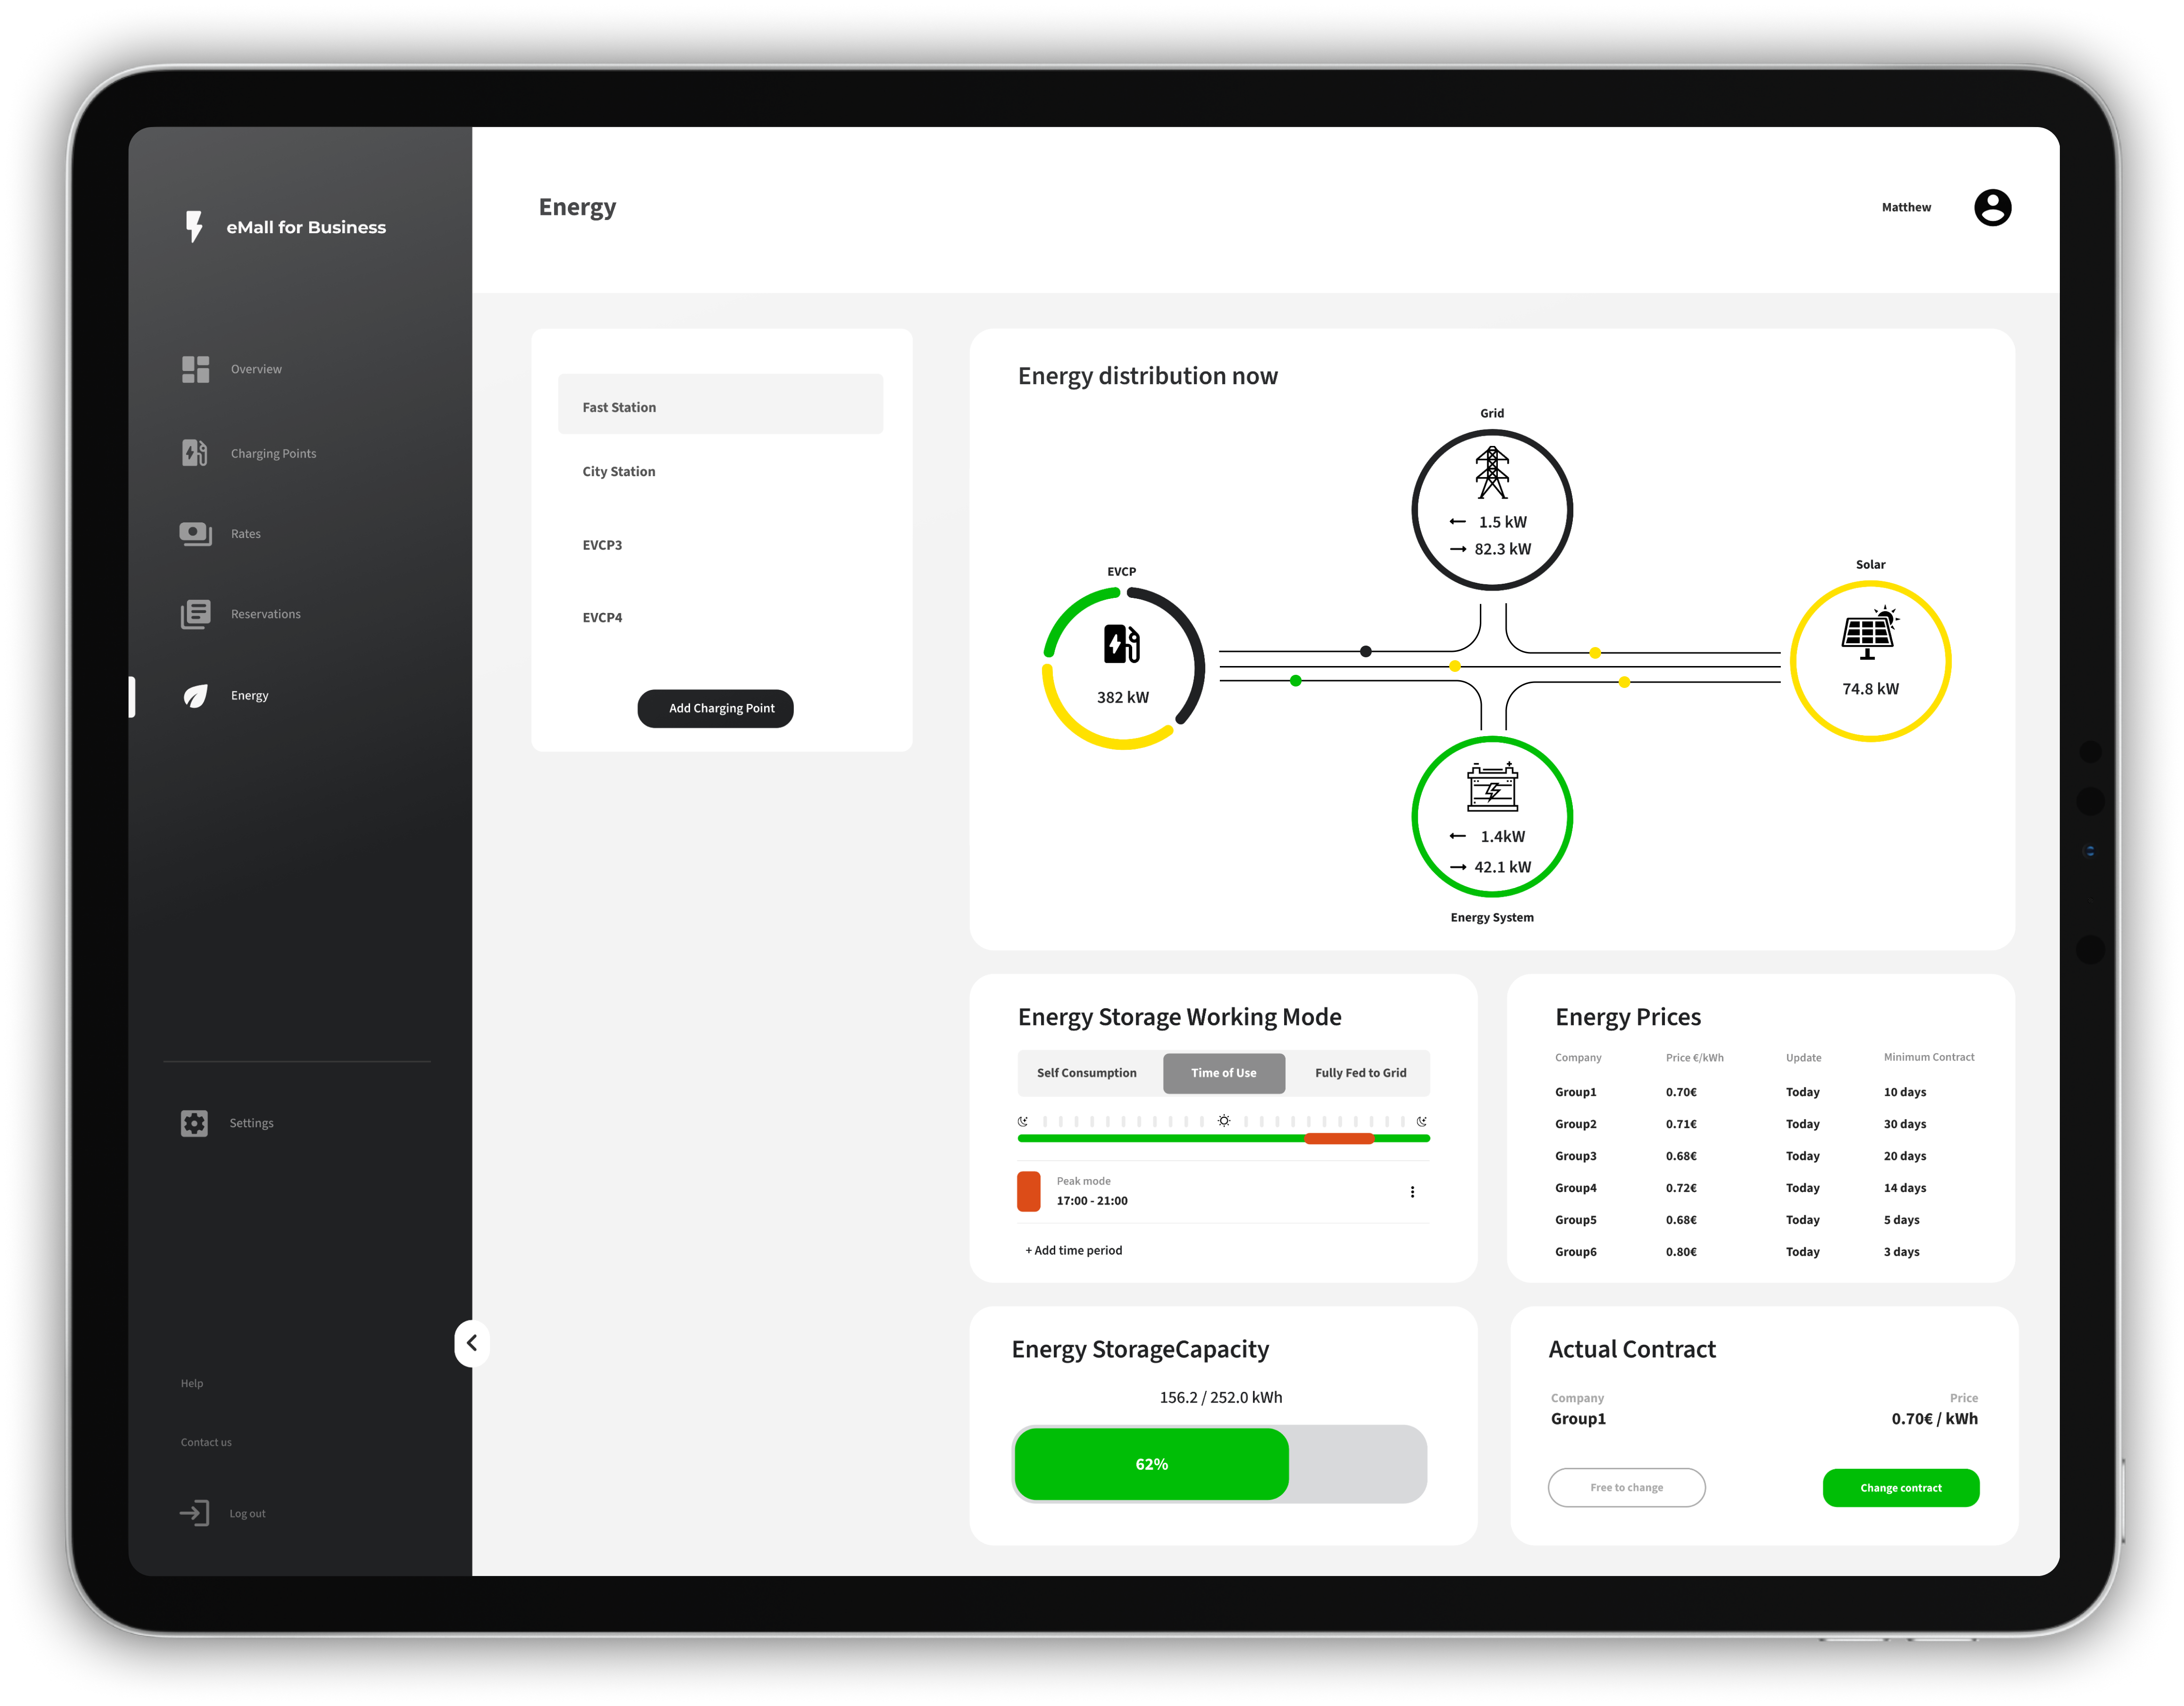
\includegraphics[scale=0.28]{src/mockups/business_energy.png}
    }
    \newline
\end{figure}


\subsubsection{Hardware Interfaces}
To use the system, both EV drivers and CPOs must have a mobile device or a personal computer.
Due to the outdoor expected use of the system, a smartphone will be a more suitable device
for a EV driver, instead for a CPO is suggested to use the system from a personal computer.
The system is based on the ability of gathering data from different sources, such as the CP, the battery storage that may be present in an EVCP and the battery status of an EV. These data are provided through hardware interfaces that are external
to our system, and we assume that an API let the system access to these data

\subsubsection{Software Interfaces}
eMall is a web application, then a modern web browsers is the only software required

\subsubsection{Communication Interfaces}
The system requires a stable internet connection to work properly.
The backend of the system will expose a unified RESTful API to communicate
with all clients using HTTPS and TCP/IP.
\\Furthermore, the system relies on various external interfaces accessible via uniform web API. These services are:
\begin{itemize}
    \item \textbf{Map Service}: eMall system relies on a map service to get the map and to do operations on the map which is the central component of the application.
    \item \textbf{GPS Service}: eMall system relies on GPS to obtain the location of the user and to show their position on the map
    \item \textbf{DSO Energy Pricing Service}: eMall system use this interface to obtain updated prices of the different DSOs available for the location of the EVCPs. The interface also, permits to select from which DSO acquire energy.
    \item \textbf{EV Service}: eMall system uses this interface that has a register that contains data about all the EVs around the world as the model, the manufacturer, the battery capacity, the efficiency, the range, the connector type and the maximum input power. It is also used to show the battery status of the user's car
    \item \textbf{OCPP compliant CP client}: eMall system relies on it to retrieve data or send data to the CPs
    \item \textbf{Calendar OS API}: The interface is used to identify which are the commitments and which are the free slots and suggest proactively when is more convenient to charge
    \item \textbf{Payment Gateway}: eMall system relies on it for processing every payment operation on the application
    \item \textbf{Push Notification Service}: eMall notifications will be sent to update in real time the EV driver that the charging shift will begin shortly, when the charging process has ended and of special offer in nearby CPs
    \item \textbf{SMS Service}: eMall system relies on it to send verification code SMS to customers phones.
\end{itemize}

\subsection{Functional Requirements}
In this section a top-down approach is followed. We provide first use cases diagrams, for each use case we provide a detailed description of the interaction and a sequence diagram. Then the list of functional requirements is built along with the mapping on both goals and use cases for traceability reasons.


\subsubsection{Use case diagrams}

\vspace*{3cm}
\begin{figure}[H]
    \centering
    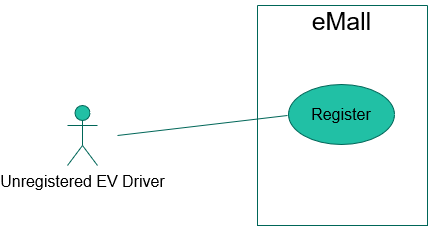
\includegraphics[scale=0.6]{src/use_case_diagram/driver_registration.png}
    \caption{Unregistered EV Driver use case diagram}
\end{figure}
\vspace*{3cm}
\begin{figure}[H]
    \centering
    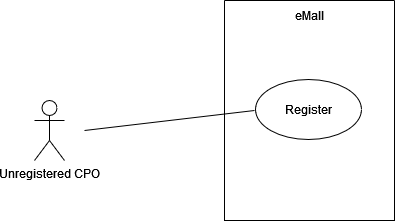
\includegraphics[scale=0.6]{src/use_case_diagram/cpo_registration.png}
    \caption{Unregistered CPO use case diagram}
\end{figure}

\begin{figure}[hp]
    \centering
    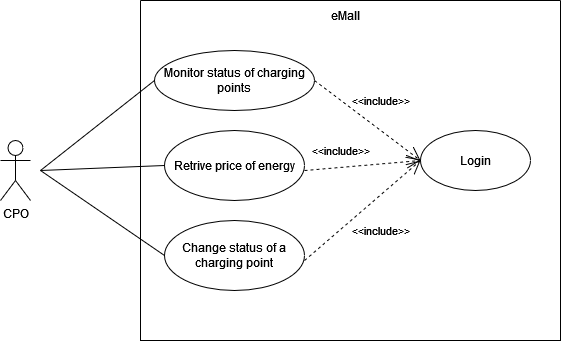
\includegraphics[scale=0.5]{src/use_case_diagram/cpo.png}
    \caption{CPO use case diagram}
\end{figure}

\begin{figure}[hp]
    \centering
    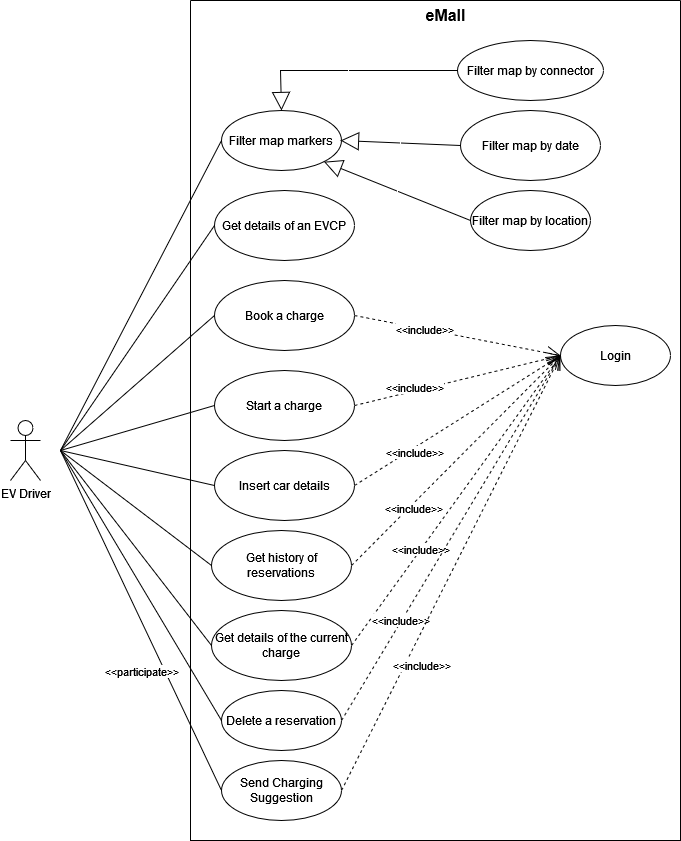
\includegraphics[scale=0.6]{src/use_case_diagram/driver.png}
    \caption{EV Driver use case diagram}
\end{figure}

\pagebreak

\subsubsection{Use cases}
In all the following use cases and sequence diagrams, the System To Be is shown as a black box interacting with the world, that is users and external API.
\usecase
{
    \begin{figure}[H]
        \centering
        \includegraphics[scale=0.9]{src/sequence_diagram/login.png}
    \end{figure}
}
{1}
{Login}
{EV driver, CPO}
{The actor is already registered in the system}
{
    \begin{enumerate}
        \item The actor requires the Login Page
        \item The system shows the Login Page to the actor
        \item The actor inserts credentials and send it to the system
        \item The system processes the information and shows a success message redirecting the user to the homepage
    \end{enumerate}
}
{The actor is logged and the homepage is displayed}
{
    \begin{itemize}
        \item A wrong username or password is submitted
    \end{itemize}
}
{
    All the exception are treated the same: the system will notify user with a human-readable message
}

\usecase
{
}
{2.1}
{CPO registration} % name
{CPO, SMS Service} % actor
{CPO clicks 'Sign Up' in the business dedicated application homepage} % entry condition
{ % event flow
    \begin{enumerate}
        \item The system sends operator the registration form
        \item Operator enters company name, VAT, IBAN, and password. Then submits the data upon reading and accepting the Privacy Policy and the Terms of Service
        \item The system calls SMS Service API to send to the CPO an SMS containing a secret code
        \item The SMS Service replies sending the SMS to the operator
        \item The operator submits the received verification code
        \item The system processes the provided information and displays a success message
    \end{enumerate}
}
{A new operator account is created} % exit condition
{ % exceptions
    \begin{itemize}
        \item A required registration field is missing when the form is submitted
        \item The operator is not associated to the given VAT
        \item A wrong verification code is submitted
        \item The timeout of verification expires
        \item Loss of internet connection
        \item The actor cancels the operation
    \end{itemize}
}
{ % notes
    All the exception are treated the same: the system will notify operator with a human-readable message and the system asks to retry
}

\usecase
{
    \begin{figure}[H]
        \centering
        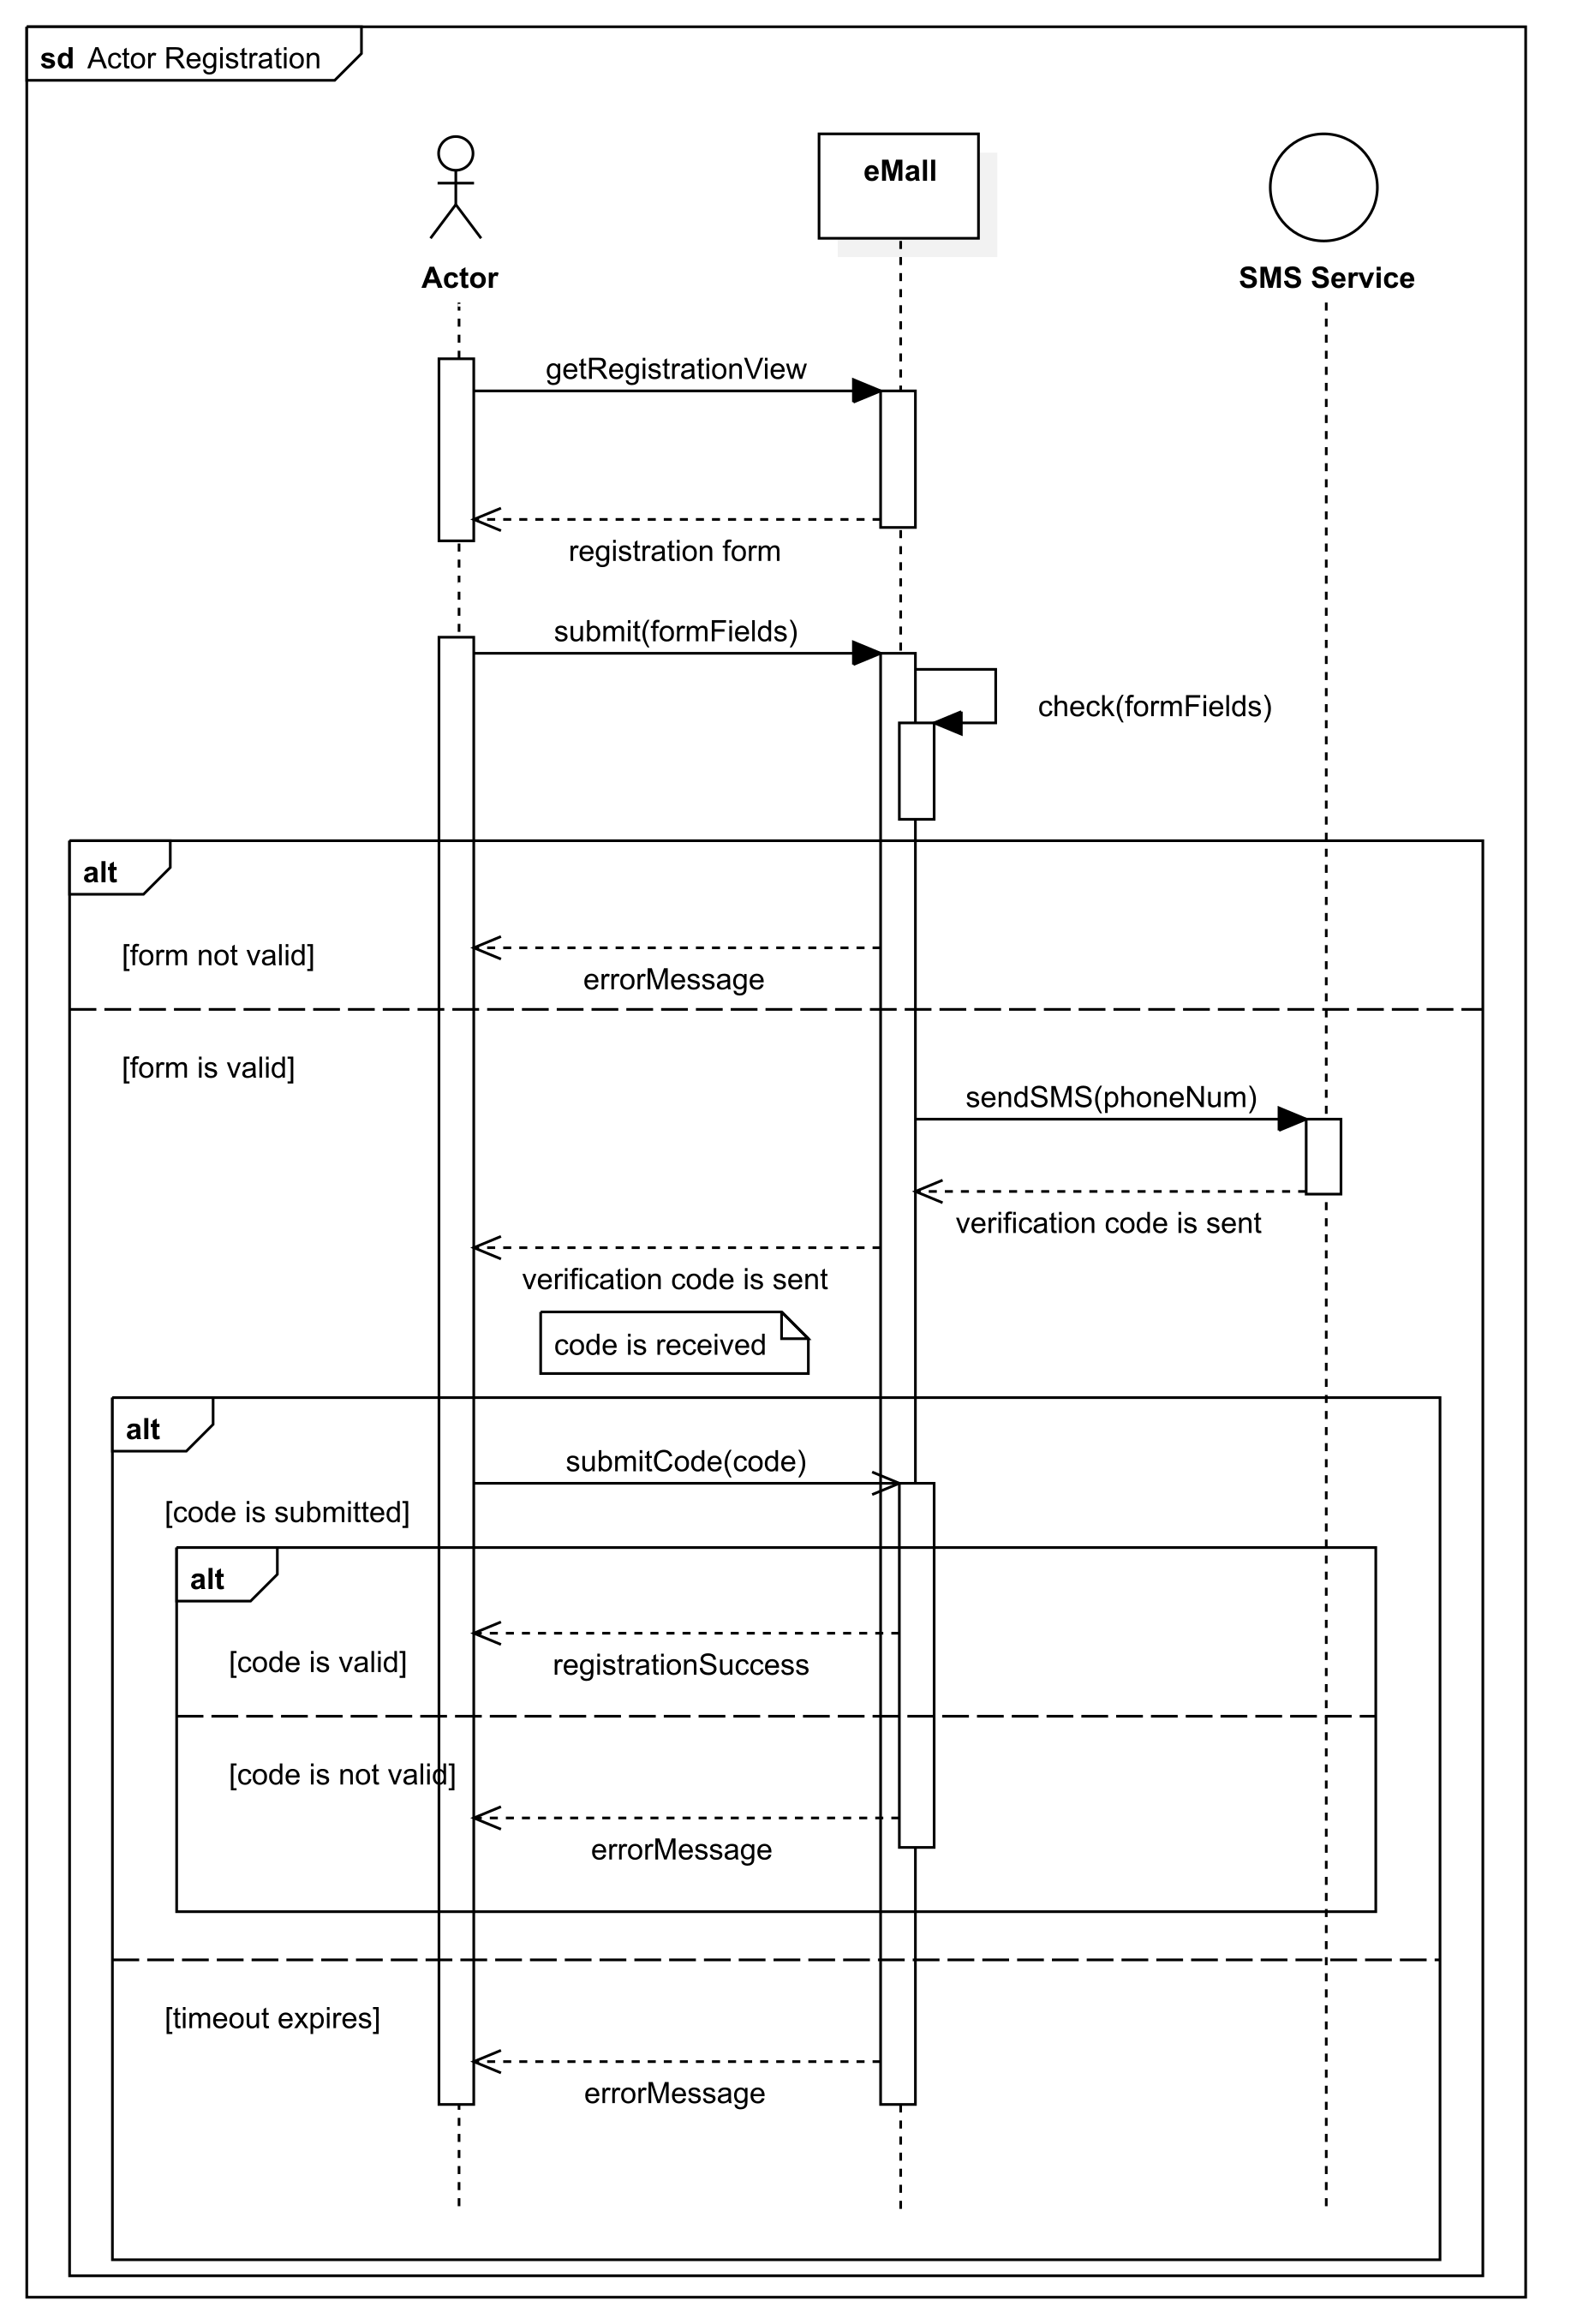
\includegraphics[scale=0.9]{src/sequence_diagram/ActorRegistration.png}
    \end{figure}
}
{2.2}
{EV driver registration}
{EV driver, SMS Service}
{EV driver clicks 'Sign Up' in the application homepage}
{
    \begin{enumerate}
        \item The system sends user the registration form
        \item Driver enters name, surname, birth date, telephone number and password. Then submits the data upon reading and accepting the Privacy Policy and the Terms of Service
        \item The system calls SMS Service API to send to the driver an SMS containing a secret code
        \item The SMS Service sends the SMS to the driver
        \item The driver submits the received verification code
        \item The system verifies the code and displays a success message
    \end{enumerate}
}
{A new EV driver account is created}
{
    \begin{itemize}
        \item A required registration field is missing when the form is submitted
        \item A wrong verification code is submitted
        \item The timeout of verification expires
        \item Loss of internet connection
        \item The actor cancels the operation
    \end{itemize}
}
{
    All the exception are treated the same: the system will notify user with a human-readable message and the user is redirected to the homepage
}


\usecase
{

}
{3.1}
{Map filtering by date}
{EV driver, Map Service}
{EV driver is in the map page}
{
    \begin{enumerate}
        \item Driver selects a date from the search bar calendar
        \item The system filters the CPs that have at least one available spot in the provided date and calls the Map Service
        \item The Map Service updates the map
    \end{enumerate}
}
{The filtered markers are displayed}
{
    \begin{itemize}
        \item The provided date is before the actual date of searching
    \end{itemize}
}
{
    The system shows an error and shows the map as it was
}

\usecase
{
}
{3.2}
{Map filtering by connector}
{EV driver, Map Service}
{EV driver is in the map page}
{
    \begin{enumerate}
        \item Driver selects a list of connectors from the search bar connector dropdown
        \item The system filters the CPs that have at least one available spot with one of the chosen connectors and calls the Map Service
        \item The Map Service updates the map
    \end{enumerate}
}
{The filtered markers are displayed}
{
    No exception in this use case
}
{
}

\usecase
{
    \begin{figure}[H]
        \centering
        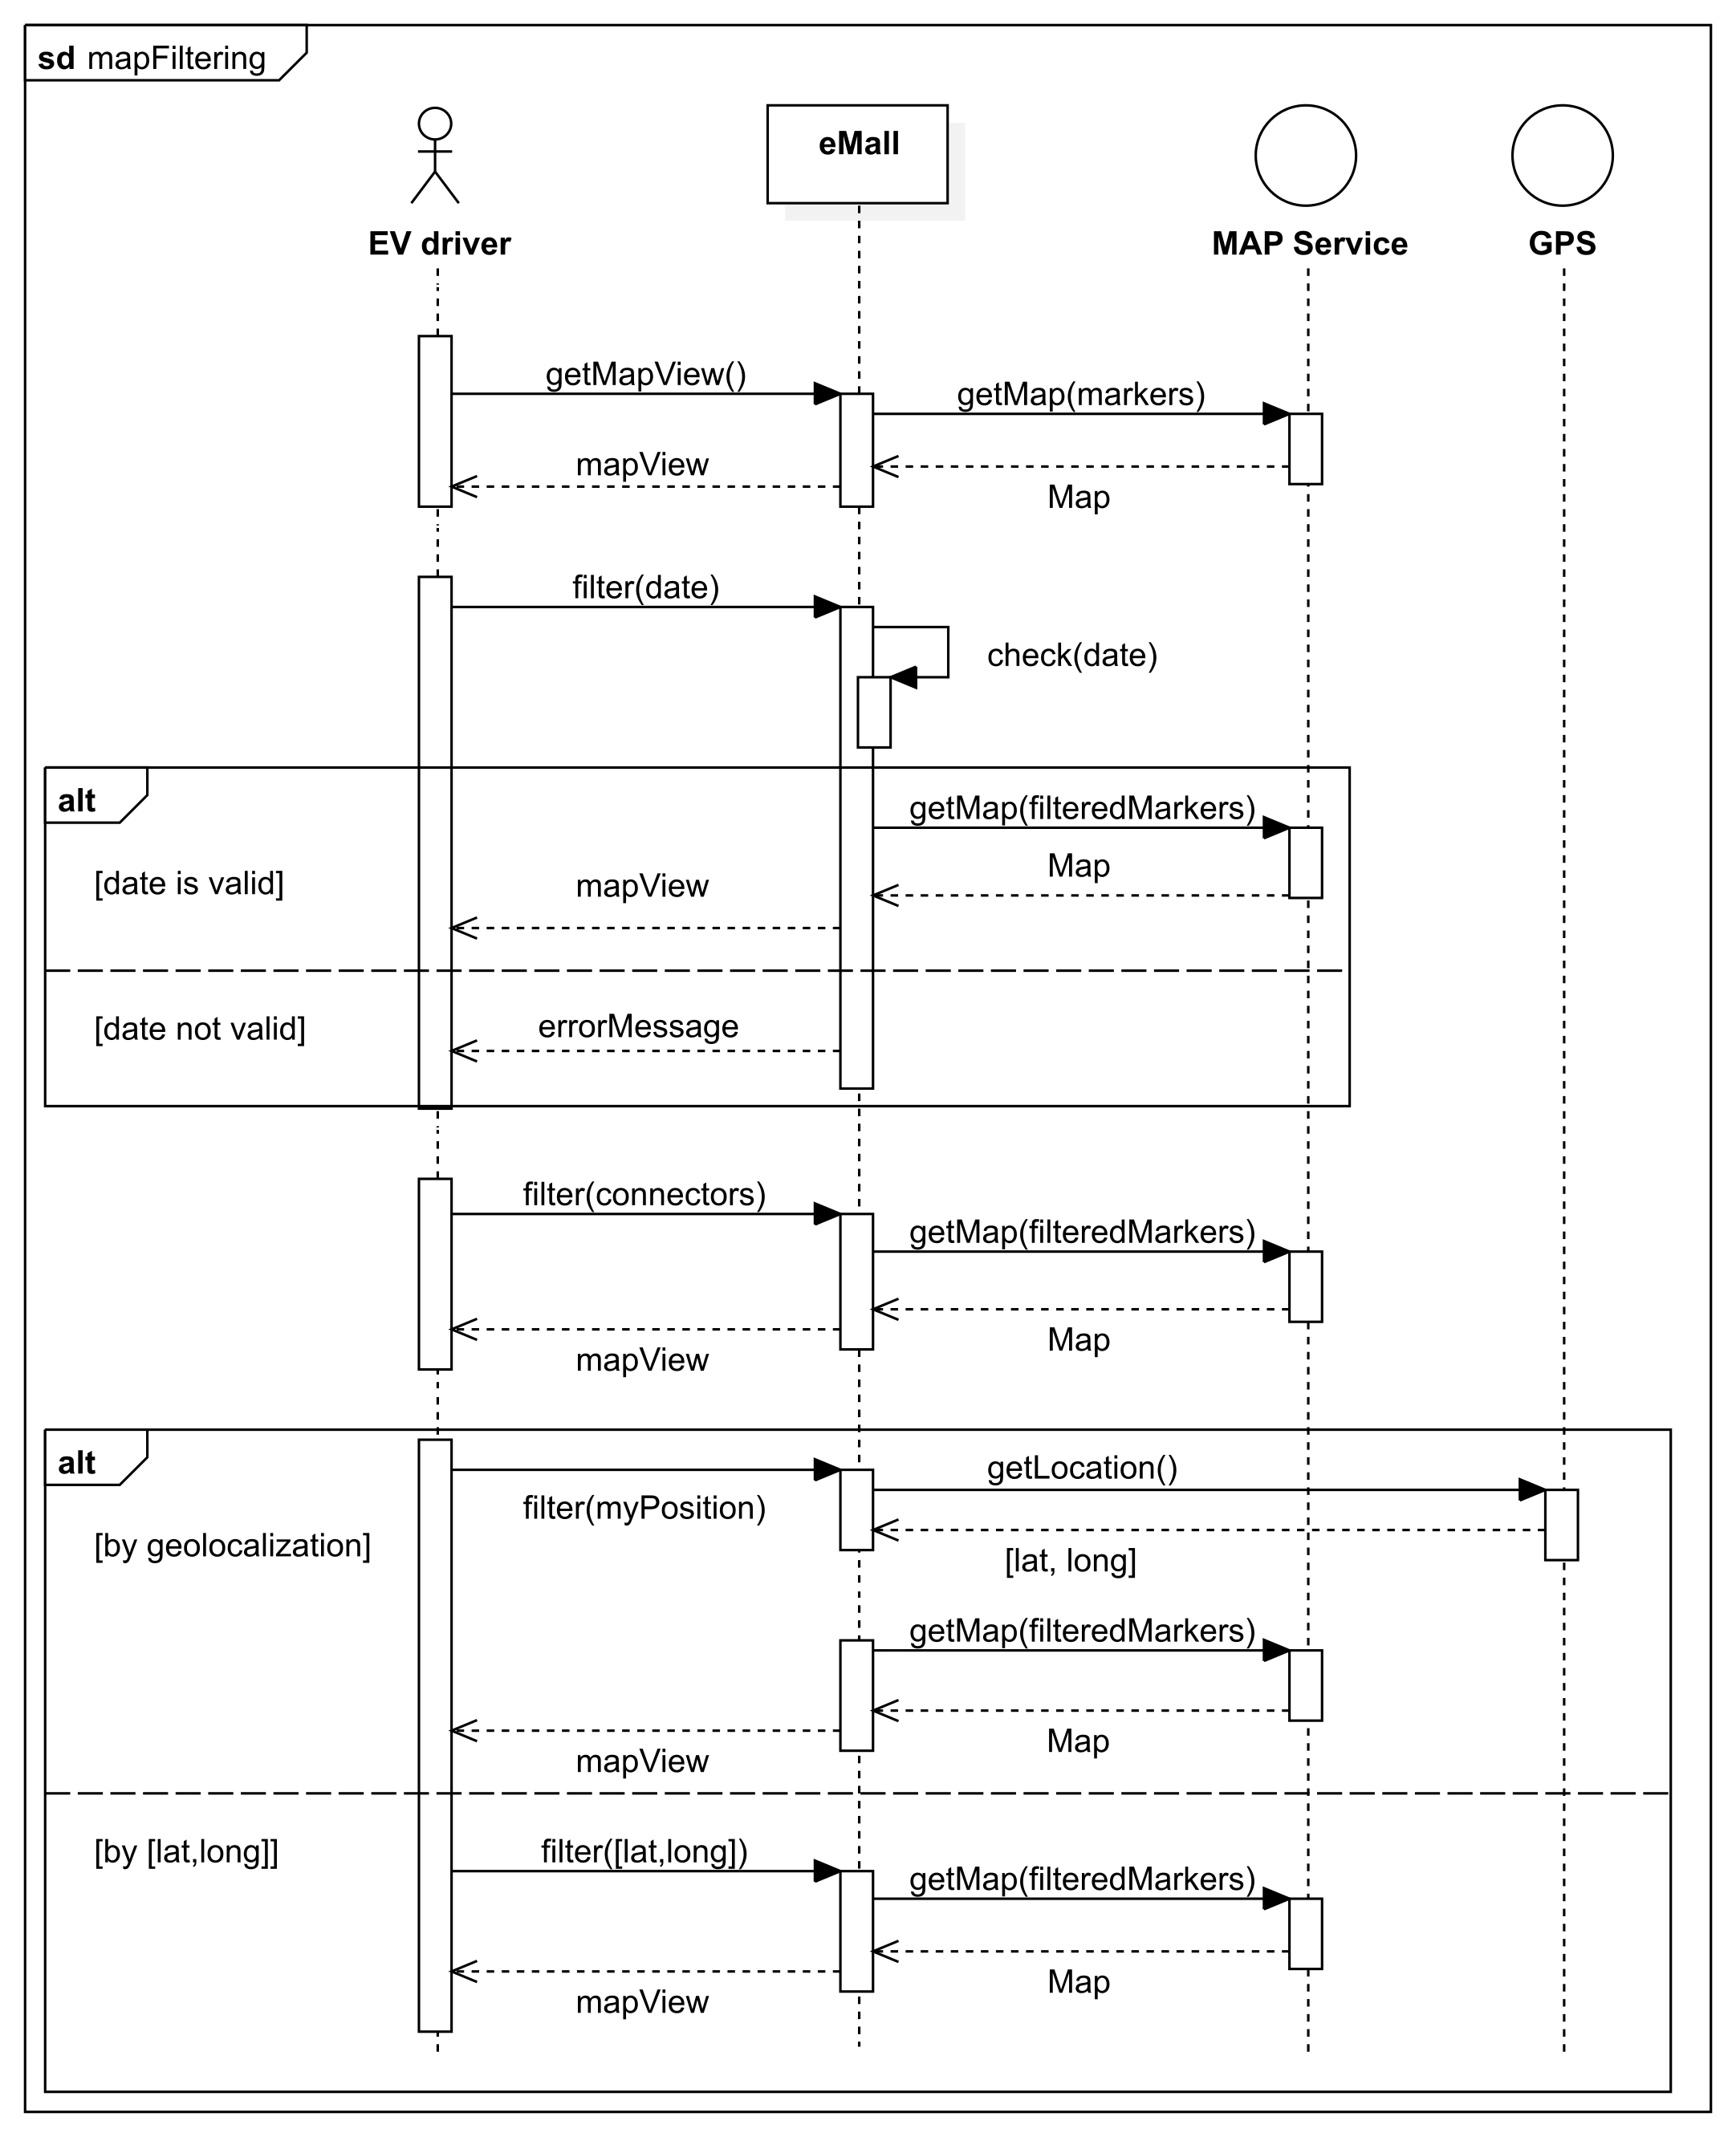
\includegraphics[scale=0.9]{src/sequence_diagram/mapFiltering.png}
    \end{figure}
}
{3.3}
{Map filtering by location}
{EV driver, Map Service, GPS Service}
{EV driver is in the map page}
{
    \begin{enumerate}
        \item Driver specifies an address where to search for CPs or their current position
        \item The system shows the CPs that are nearby the specified address and calls the Map Service
        \item The Map Service updates the map
    \end{enumerate}
}
{The filtered markers are displayed}
{
    \begin{itemize}
        \item The result of geo-localization of the specified address is not defined
    \end{itemize}
}
{
    The system shows an error and the map as it was
}

\usecase
{
    \begin{figure}[H]
        \centering
        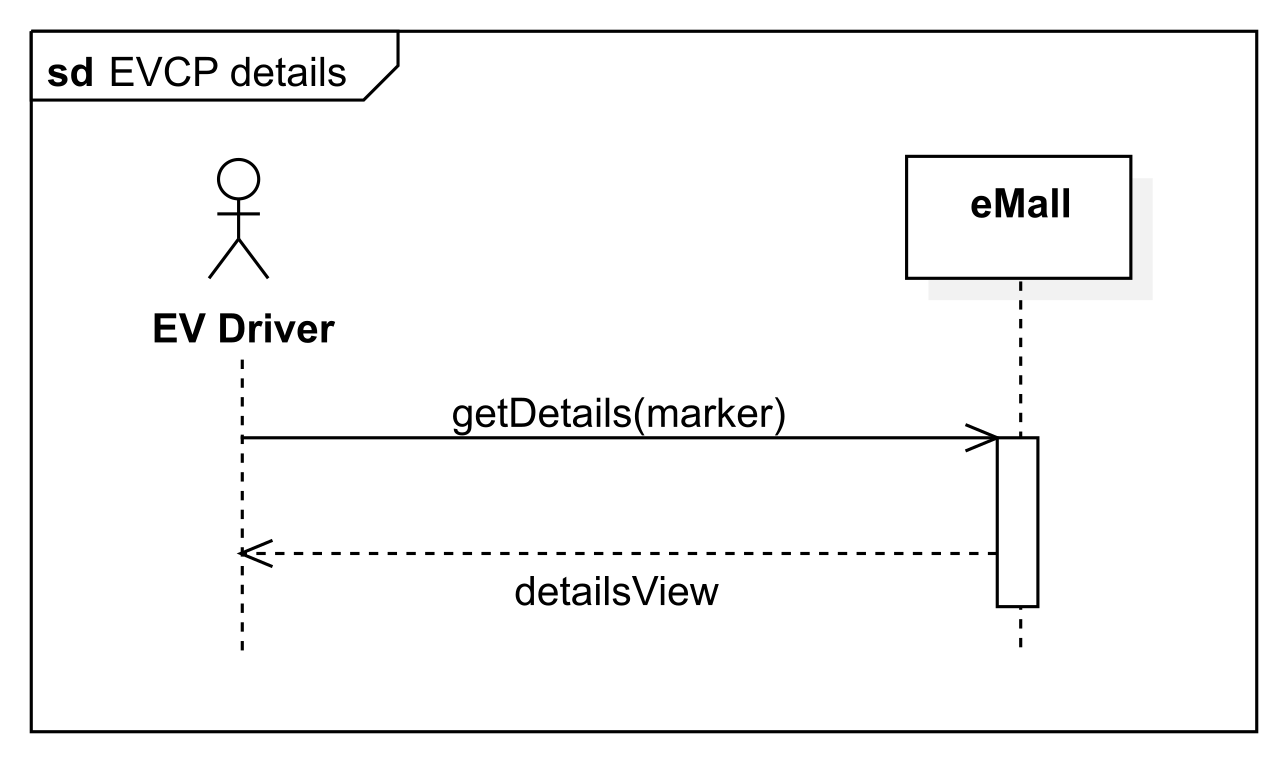
\includegraphics[scale=0.9]{src/sequence_diagram/EVCPdetails.png}
    \end{figure}
}
{4}
{Get details of an EVCP}
{EV driver}
{EV driver is in the map page}
{
    \begin{enumerate}
        \item Driver selects a marker representing an EVCP on the map
        \item The system shows the details of the EVCP associated to the marker
    \end{enumerate}
}
{A page with EVCP details is shown}
{
    No exception in this use case
}
{
}

\usecase
{
    \begin{figure}[H]
        \centering
        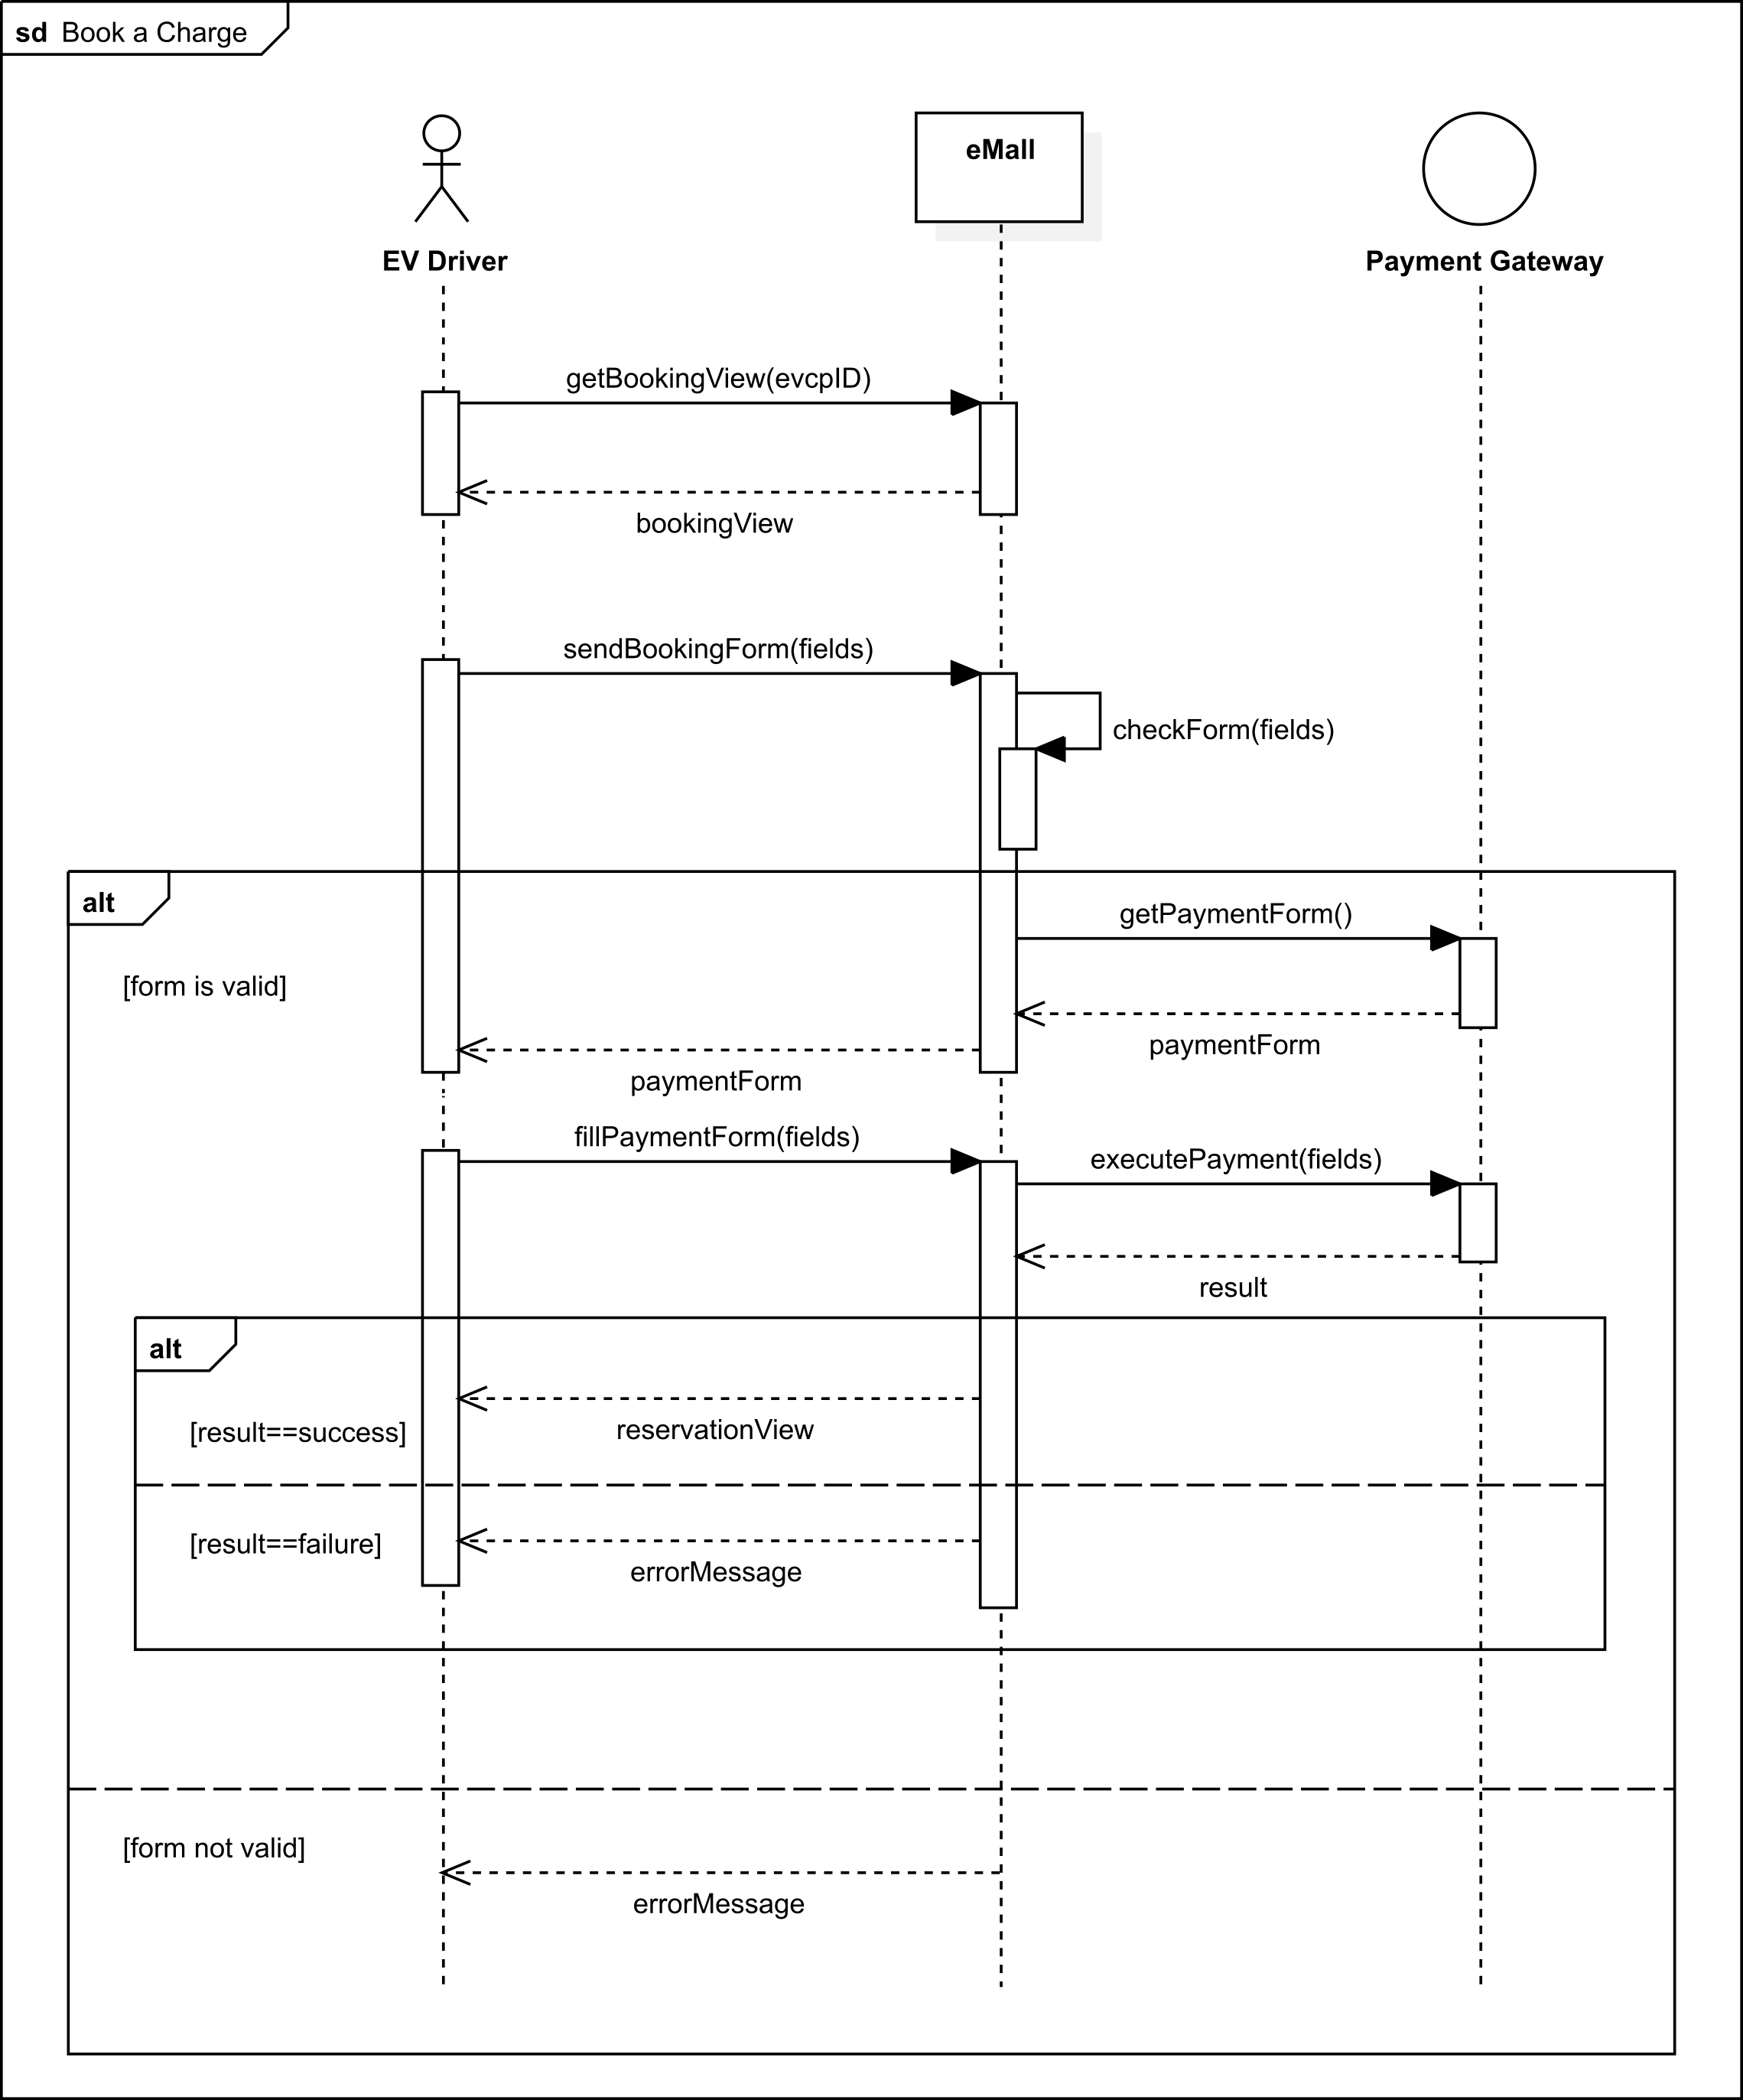
\includegraphics[scale=0.9]{src/sequence_diagram/bookCharge.png}
    \end{figure}
}
{5}
{Book a charge}
{EV driver, Payment Gateway}
{Authenticated EV driver is in the EVCP details page}
{
    \begin{enumerate}
        \item User clicks 'Book a Charge' button or one among the 'Now' buttons related to connector types (if available)
        \item The system show a booking page containing a form with connector, date and time frame selection
        \item User fills the form and clicks 'Book' button
        \item The system processes the information and redirects the user to the payment gateway interface
        \item The Payment Gateway sends user a payment form
        \item The user fills the form with payment information and clicks 'Confirm'
        \item The Payment Gateway processes the information and replies to the system with a notification
        \item The System processes the information and show a success message redirecting the user to the reservation tab
    \end{enumerate}
}
{The spot is booked and the transaction is successfully executed}
{
    \begin{itemize}
        \item At least one of the inserted booking data is not valid
        \item The payment gateway return an invalid payment
    \end{itemize}
}
{
    \begin{itemize}
        \item First Exception: the system shows an error and redirect user to EVCP details page
        \item Second Exception: the system shows an error during the payment process and asks to retry
    \end{itemize}
}

\usecase
{
    \begin{figure}[H]
        \centering
        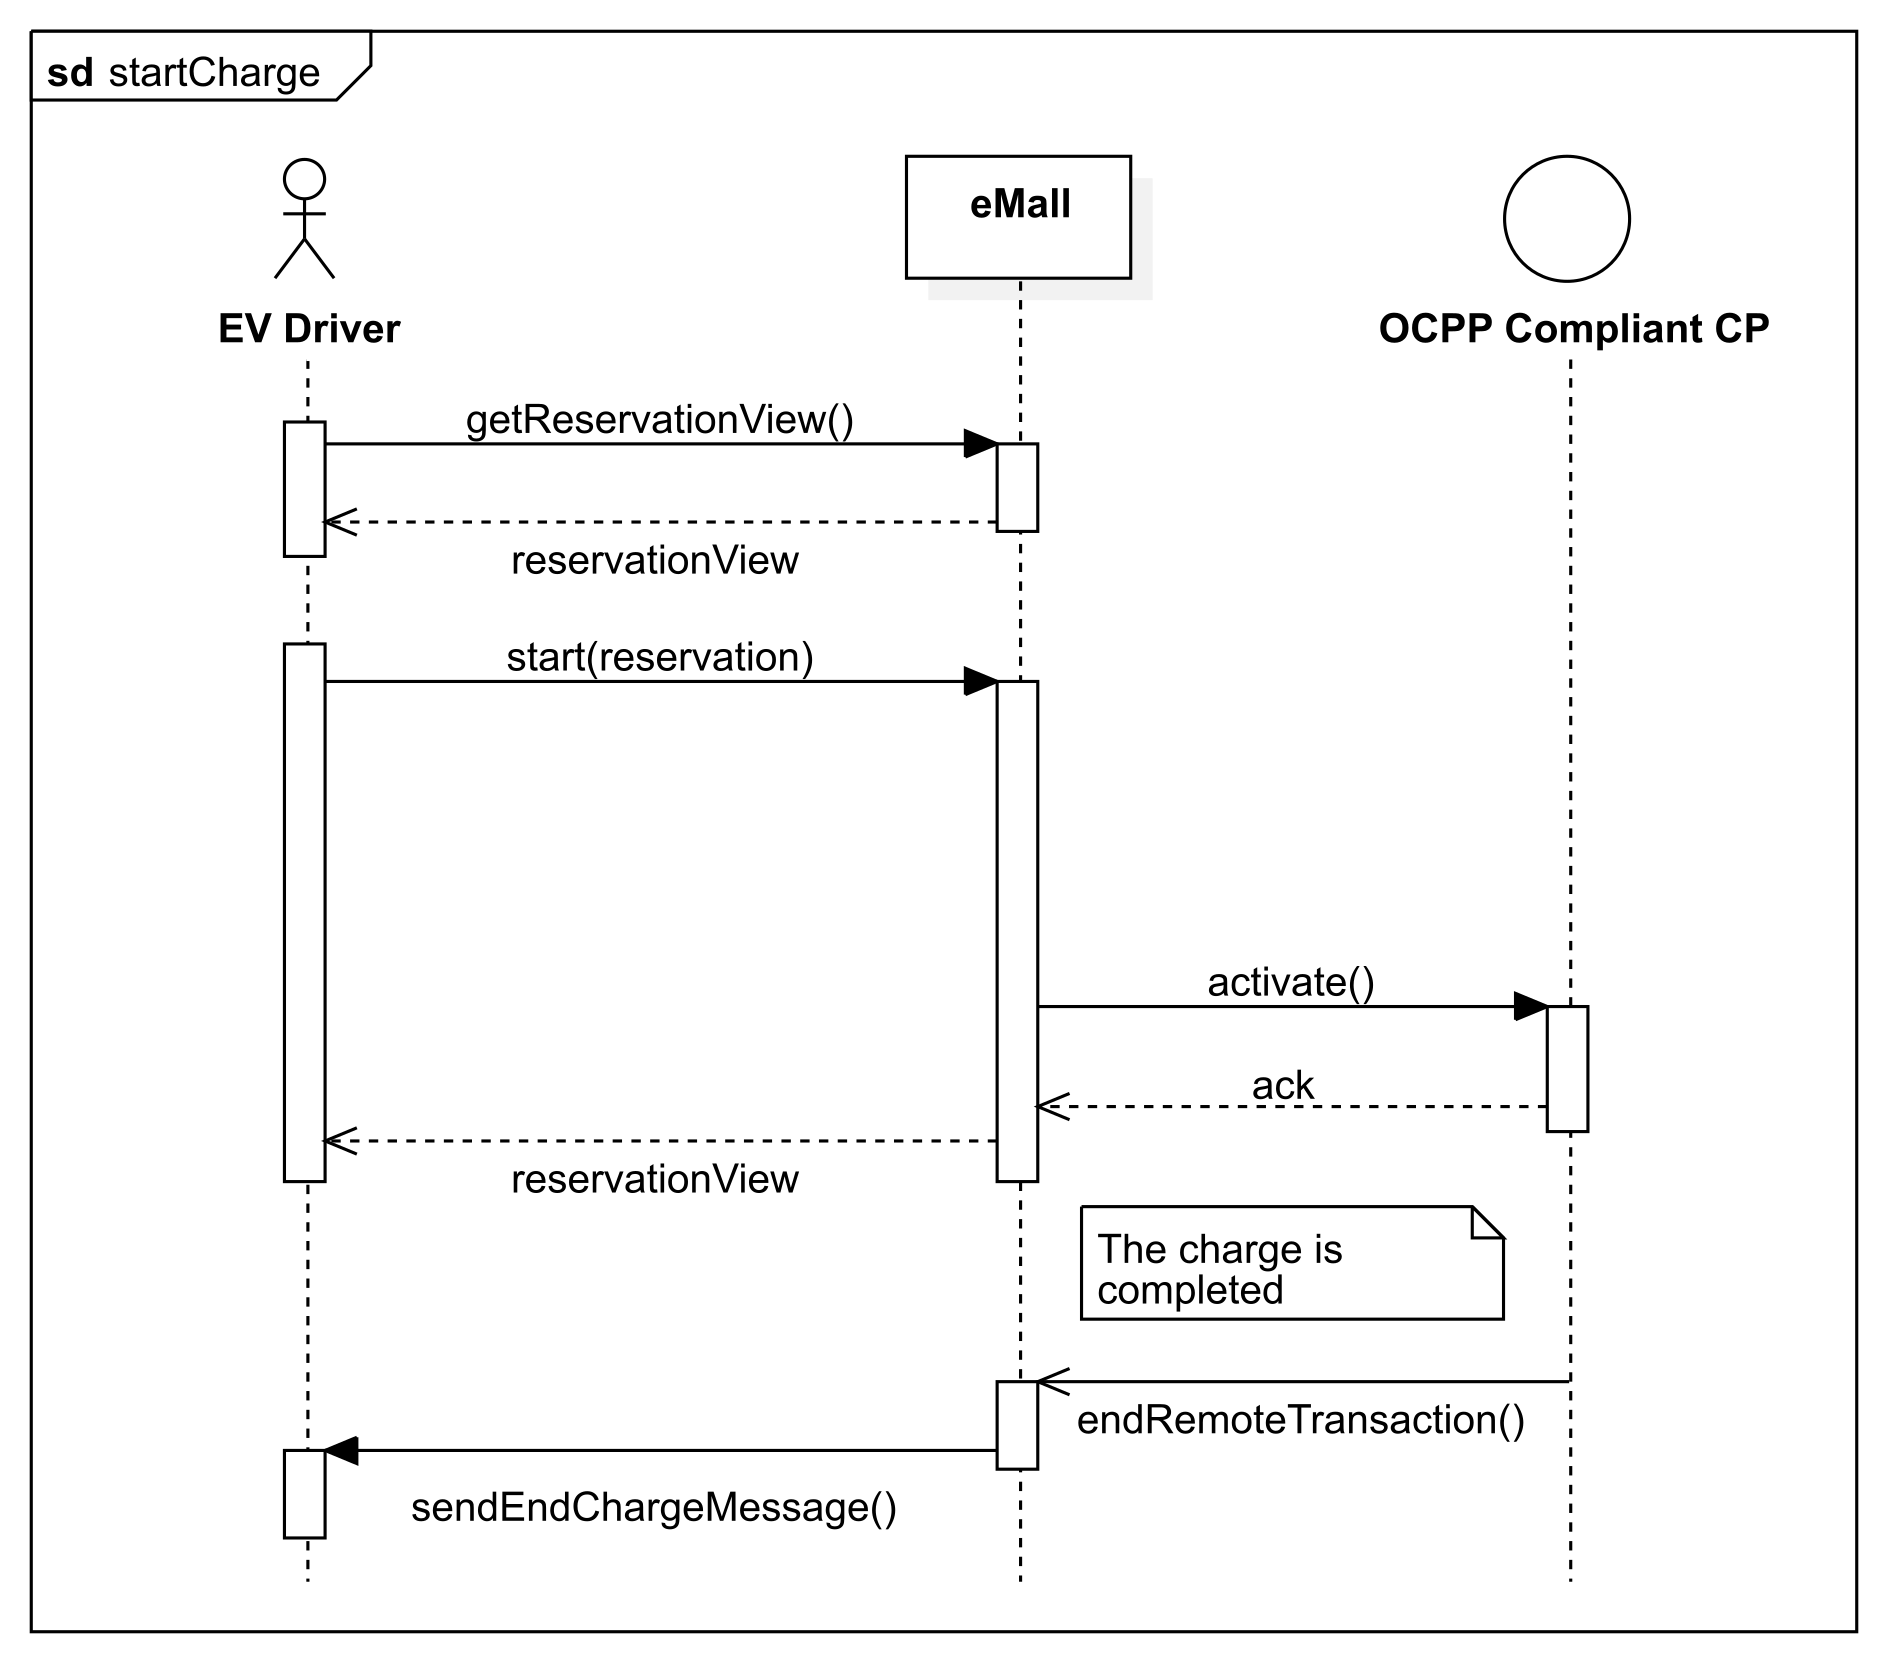
\includegraphics[scale=0.9]{src/sequence_diagram/startCharge.png}
    \end{figure}
}
{6}
{Start a charge}
{EV driver, OCPP Compliant CP client}
{Authenticated EV driver is in the reservation page}
{
    \begin{enumerate}
        \item The system shows all the reservations with the "pending" reservation in evidence
        \item User clicks the button 'Start' in the reservation in evidence to start the charge
        \item The system receives the input and activates the CP through the OCPP protocol
        \item The CP replies acknowledging the system that its status has changed from "reserved" to "charging"
        \item The system changes the status of the reservation in "running"
    \end{enumerate}
}
{The charging is started}
{
    No exception in this use case
}
{
}

\usecase
{
    \begin{figure}[H]
        \centering
        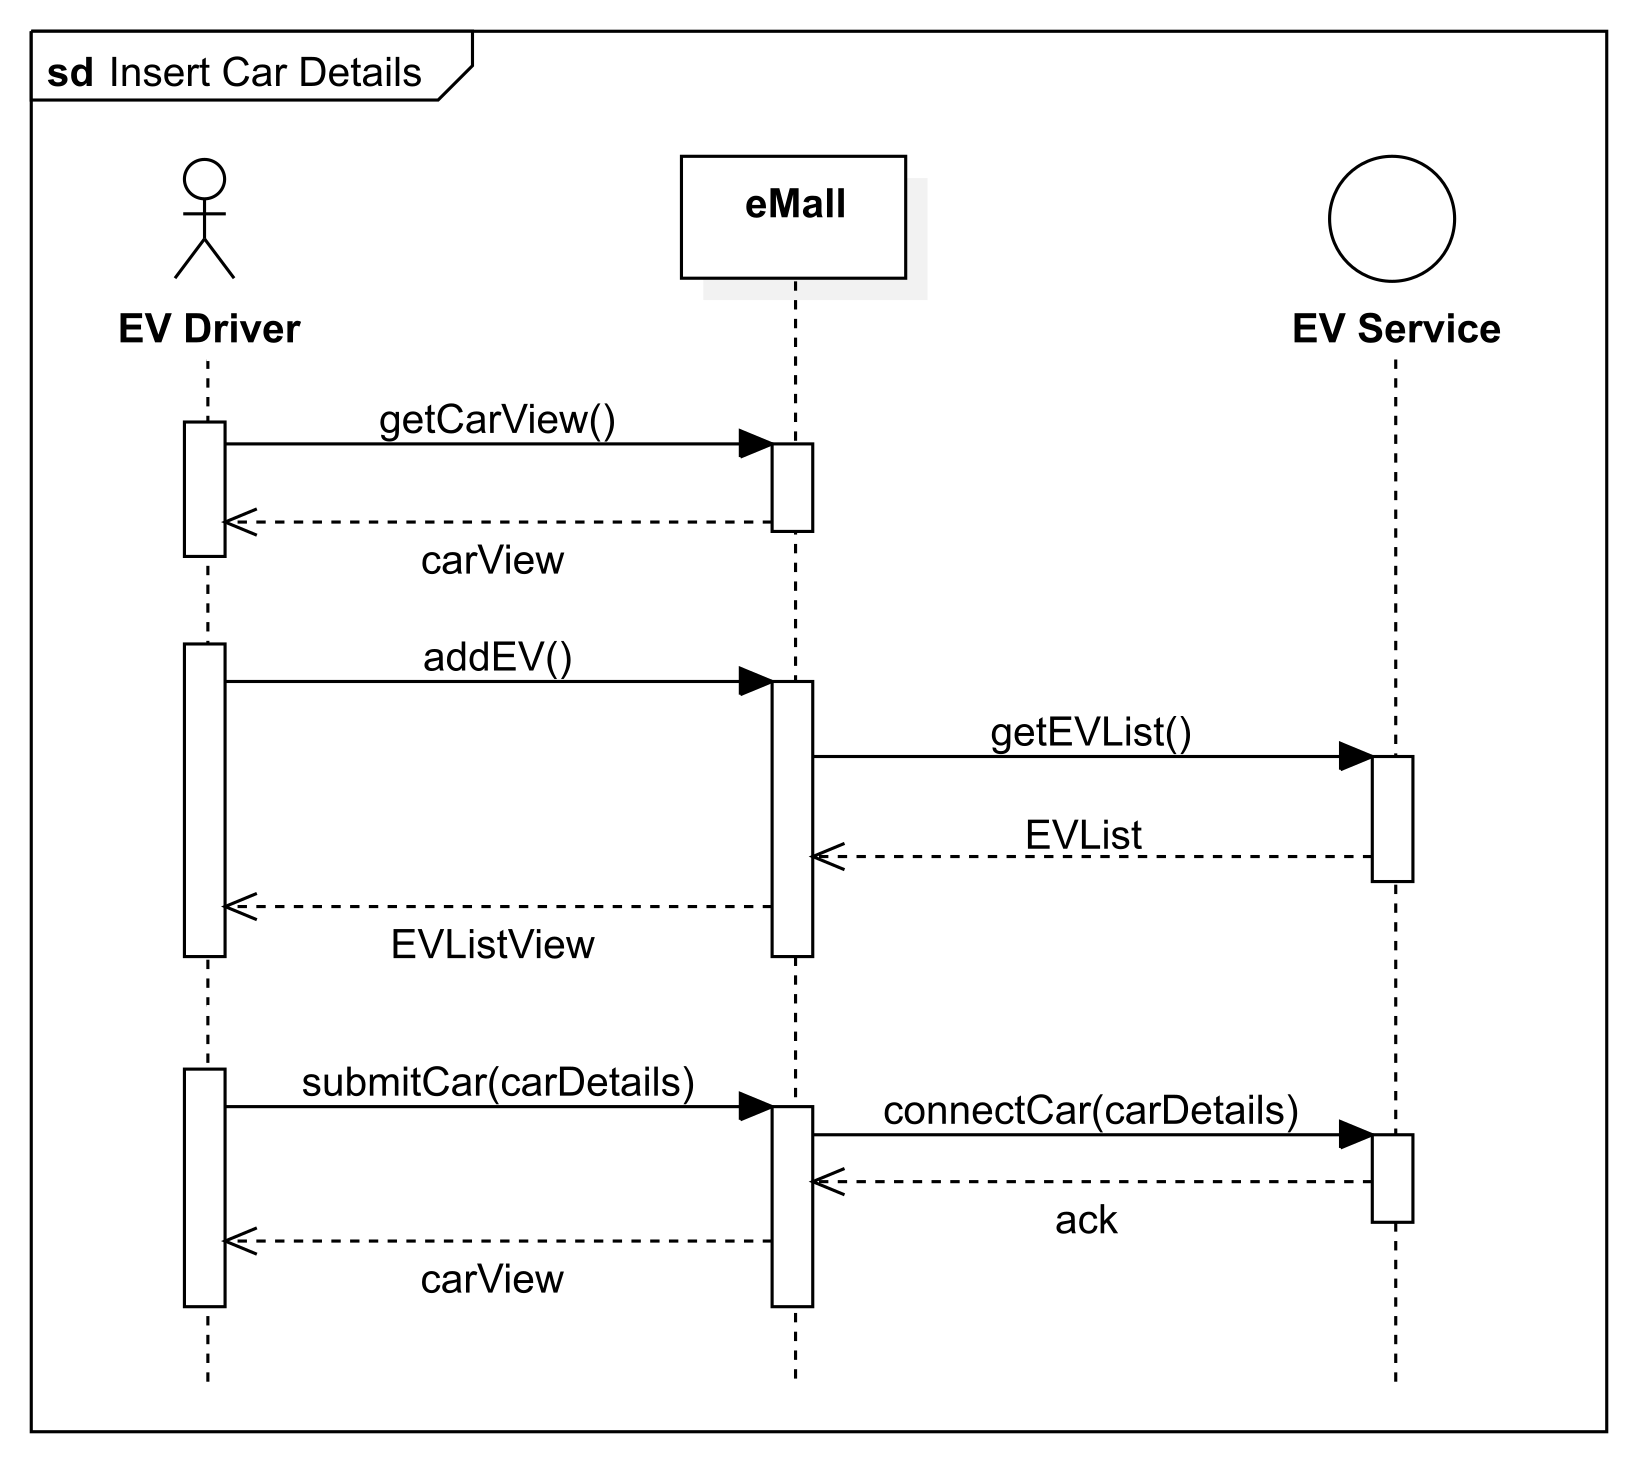
\includegraphics[scale=0.9]{src/sequence_diagram/insertCar.png}
    \end{figure}
}
{7}
{Personalize experience by inserting car details}
{EV driver, EV Service}
{Authenticated EV driver is in homepage}
{
    \begin{enumerate}
        \item The user ask the car view
        \item The system shows user the car page
        \item The user clicks 'Add an EV' button
        \item The system ask EV Service an updated list of EVCP
        \item The EV Service replies with an updated list of EV
        \item The systems shows the list of EV to user
        \item The user select one of the EV and connects the personal EV to the EV Service API
        \item The system processes the information and shows a success message
    \end{enumerate}
}
{The user has inserted car details}
{
    No exception in this use case
}
{
}

\usecase
{
    \begin{figure}[H]
        \centering
        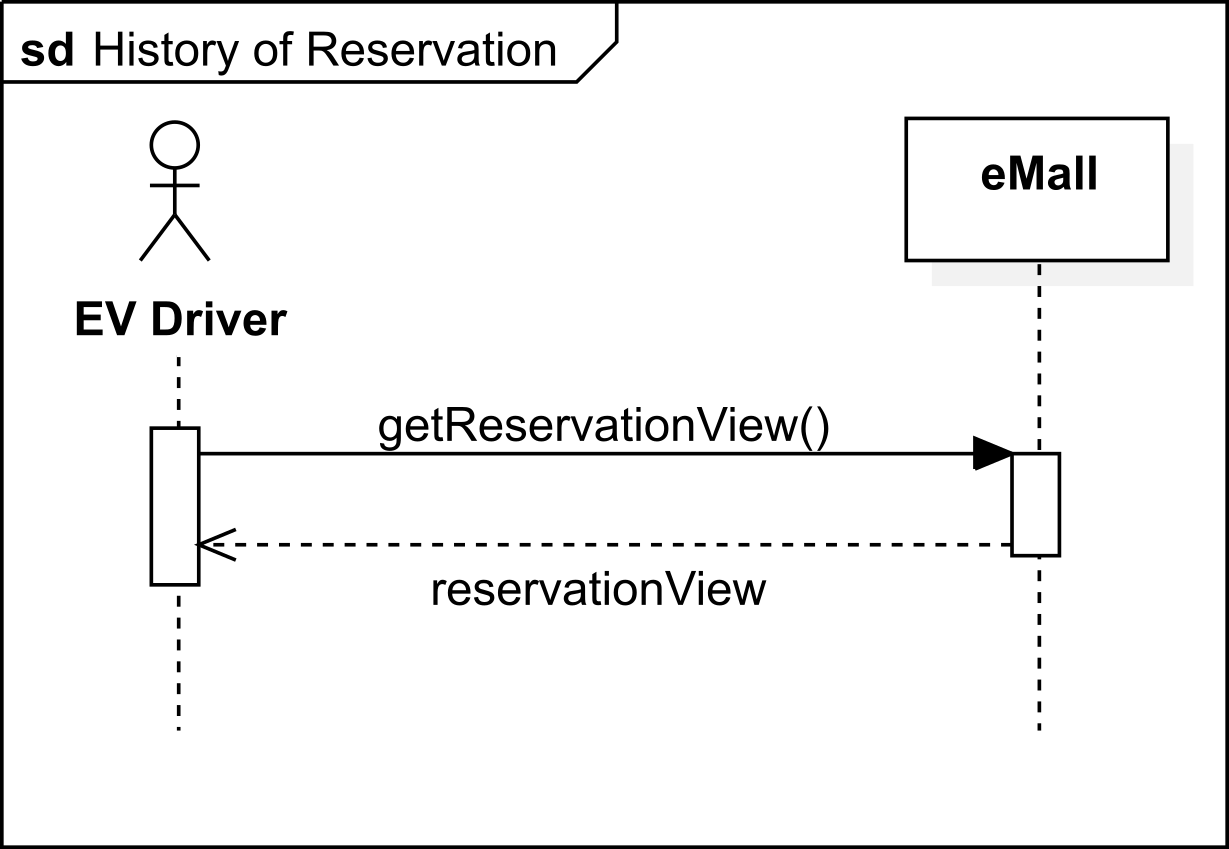
\includegraphics[scale=0.9]{src/sequence_diagram/reservationView.png}
    \end{figure}
}
{8}
{Get history of reservations}
{EV driver}
{Authenticated EV driver is in the home page}
{
    \begin{enumerate}
        \item The user switch to the reservation tab
        \item The system shows a page with a list of past reservations and active ones
    \end{enumerate}
}
{A list of reservations is shown}
{
    No exception in this use case
}
{
}

\pagebreak
\usecase
{
    \begin{figure}[H]
        \centering
        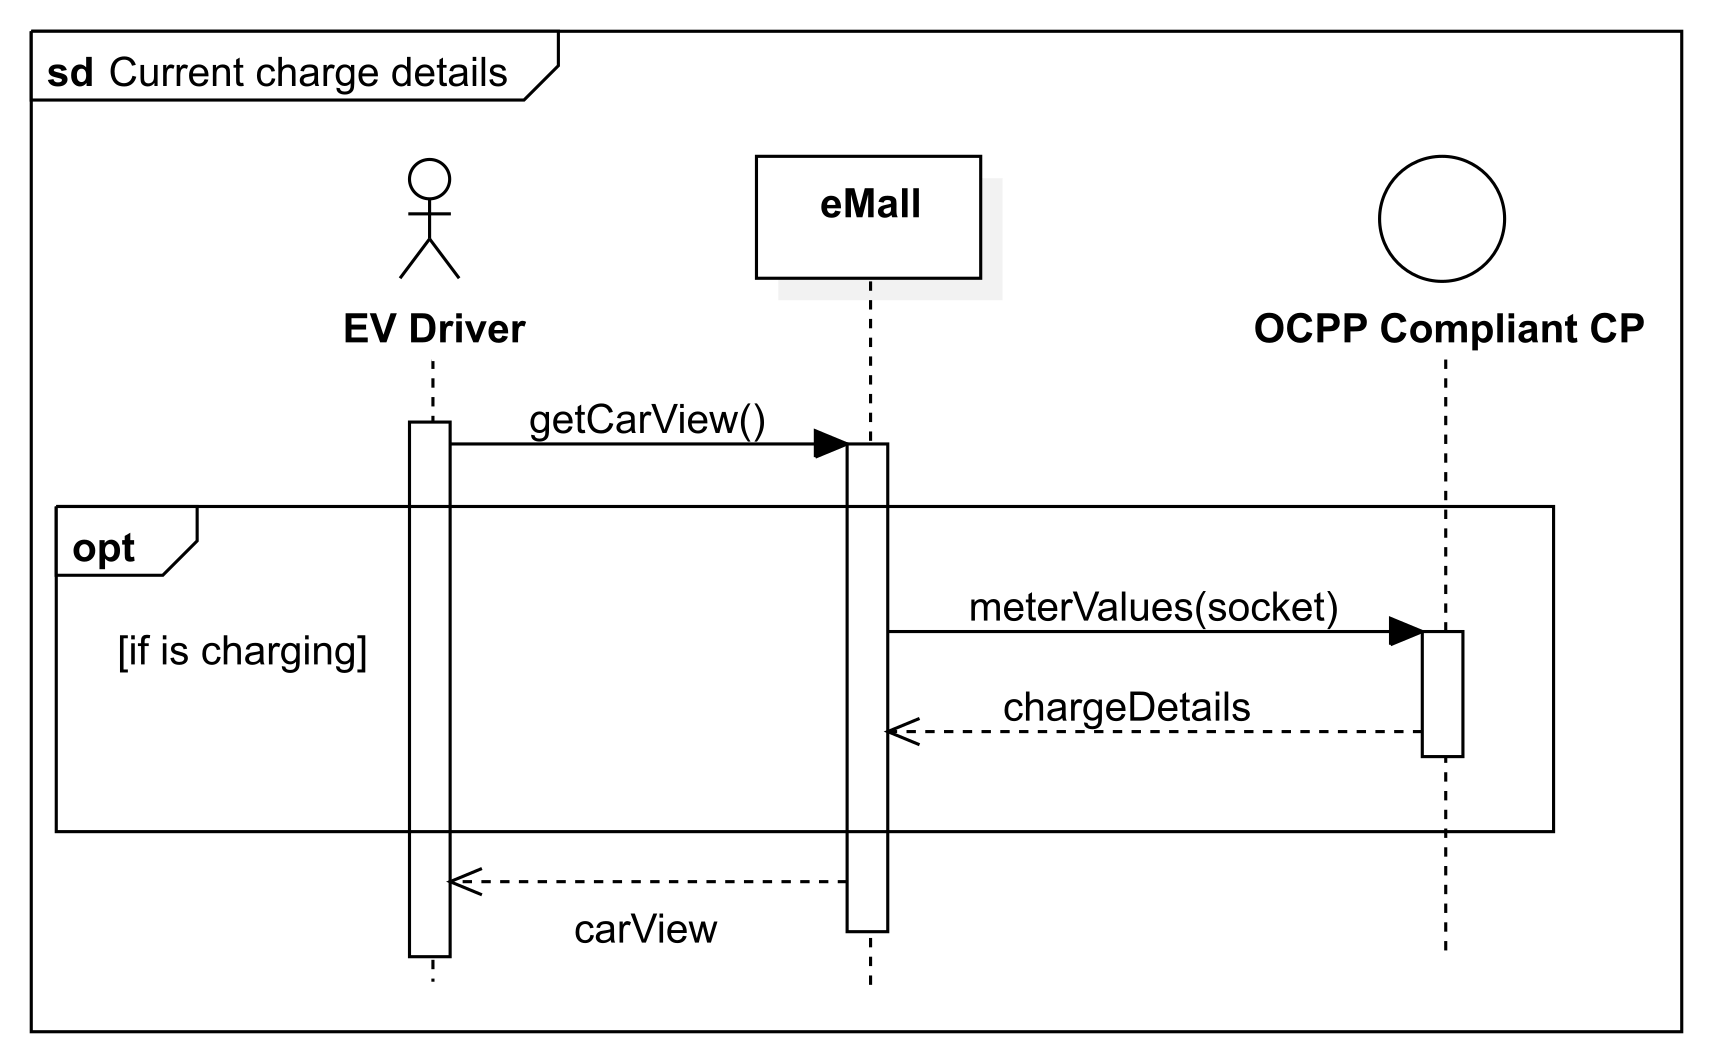
\includegraphics[scale=0.9]{src/sequence_diagram/currentChargeDetails.png}
    \end{figure}
}
{9}
{Get details of the current charge}
{EV driver, OCPP Compliant CP Client}
{Authenticated EV driver is in the car tab}
{
    \begin{enumerate}
        \item The system asks the CP, through OCPP, the details of the current charge of the user
        \item The CP replies, through OCPP, with the status
        \item The system shows all the details of the current charge
    \end{enumerate}
}
{The details of the current charge are shown}
{
    No exception in this use case
}
{
}

\usecase
{
    \begin{figure}[H]
        \centering
        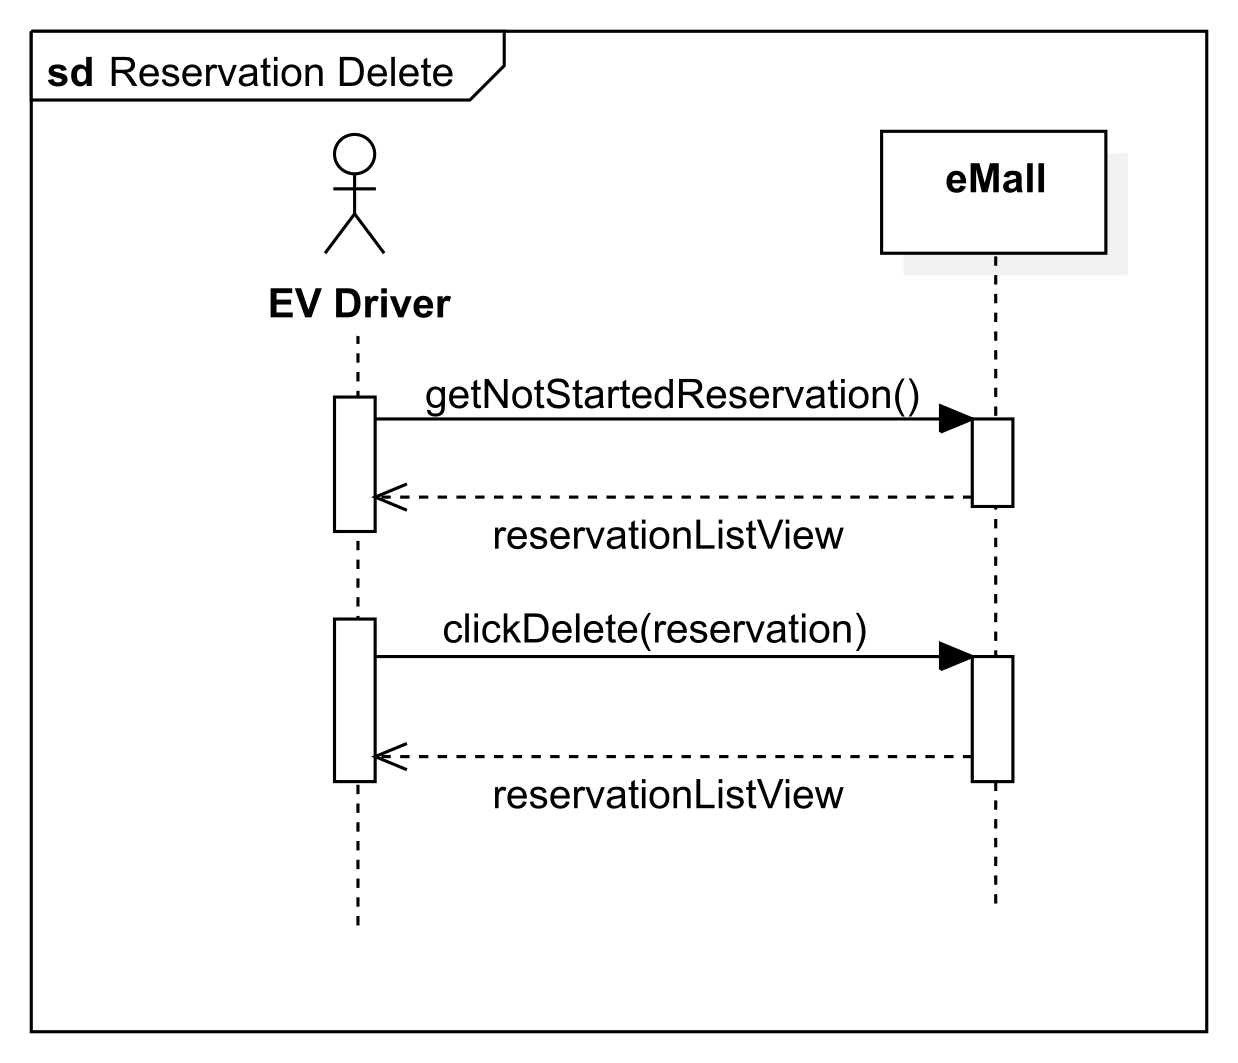
\includegraphics[scale=0.9]{src/sequence_diagram/deleteReservation.png}
    \end{figure}
}
{10}
{Delete a reservation}
{EV driver}
{Authenticated EV driver is in reservation tab}
{
    \begin{enumerate}
        \item The system shows a list with all the "not started" reservation
        \item User selects a reservation and click the associated button
        \item The system receives the input and shows details on the selected reservation
        \item User clicks "delete" button in current reservation
        \item The system displays a success message
    \end{enumerate}
}
{The user has deleted a reservation}
{
    \begin{itemize}
        \item At least one of the inserted data is not valid
    \end{itemize}
}
{
    The system shows an error asking to retry
}

\usecase
{
    \begin{figure}[H]
        \centering
        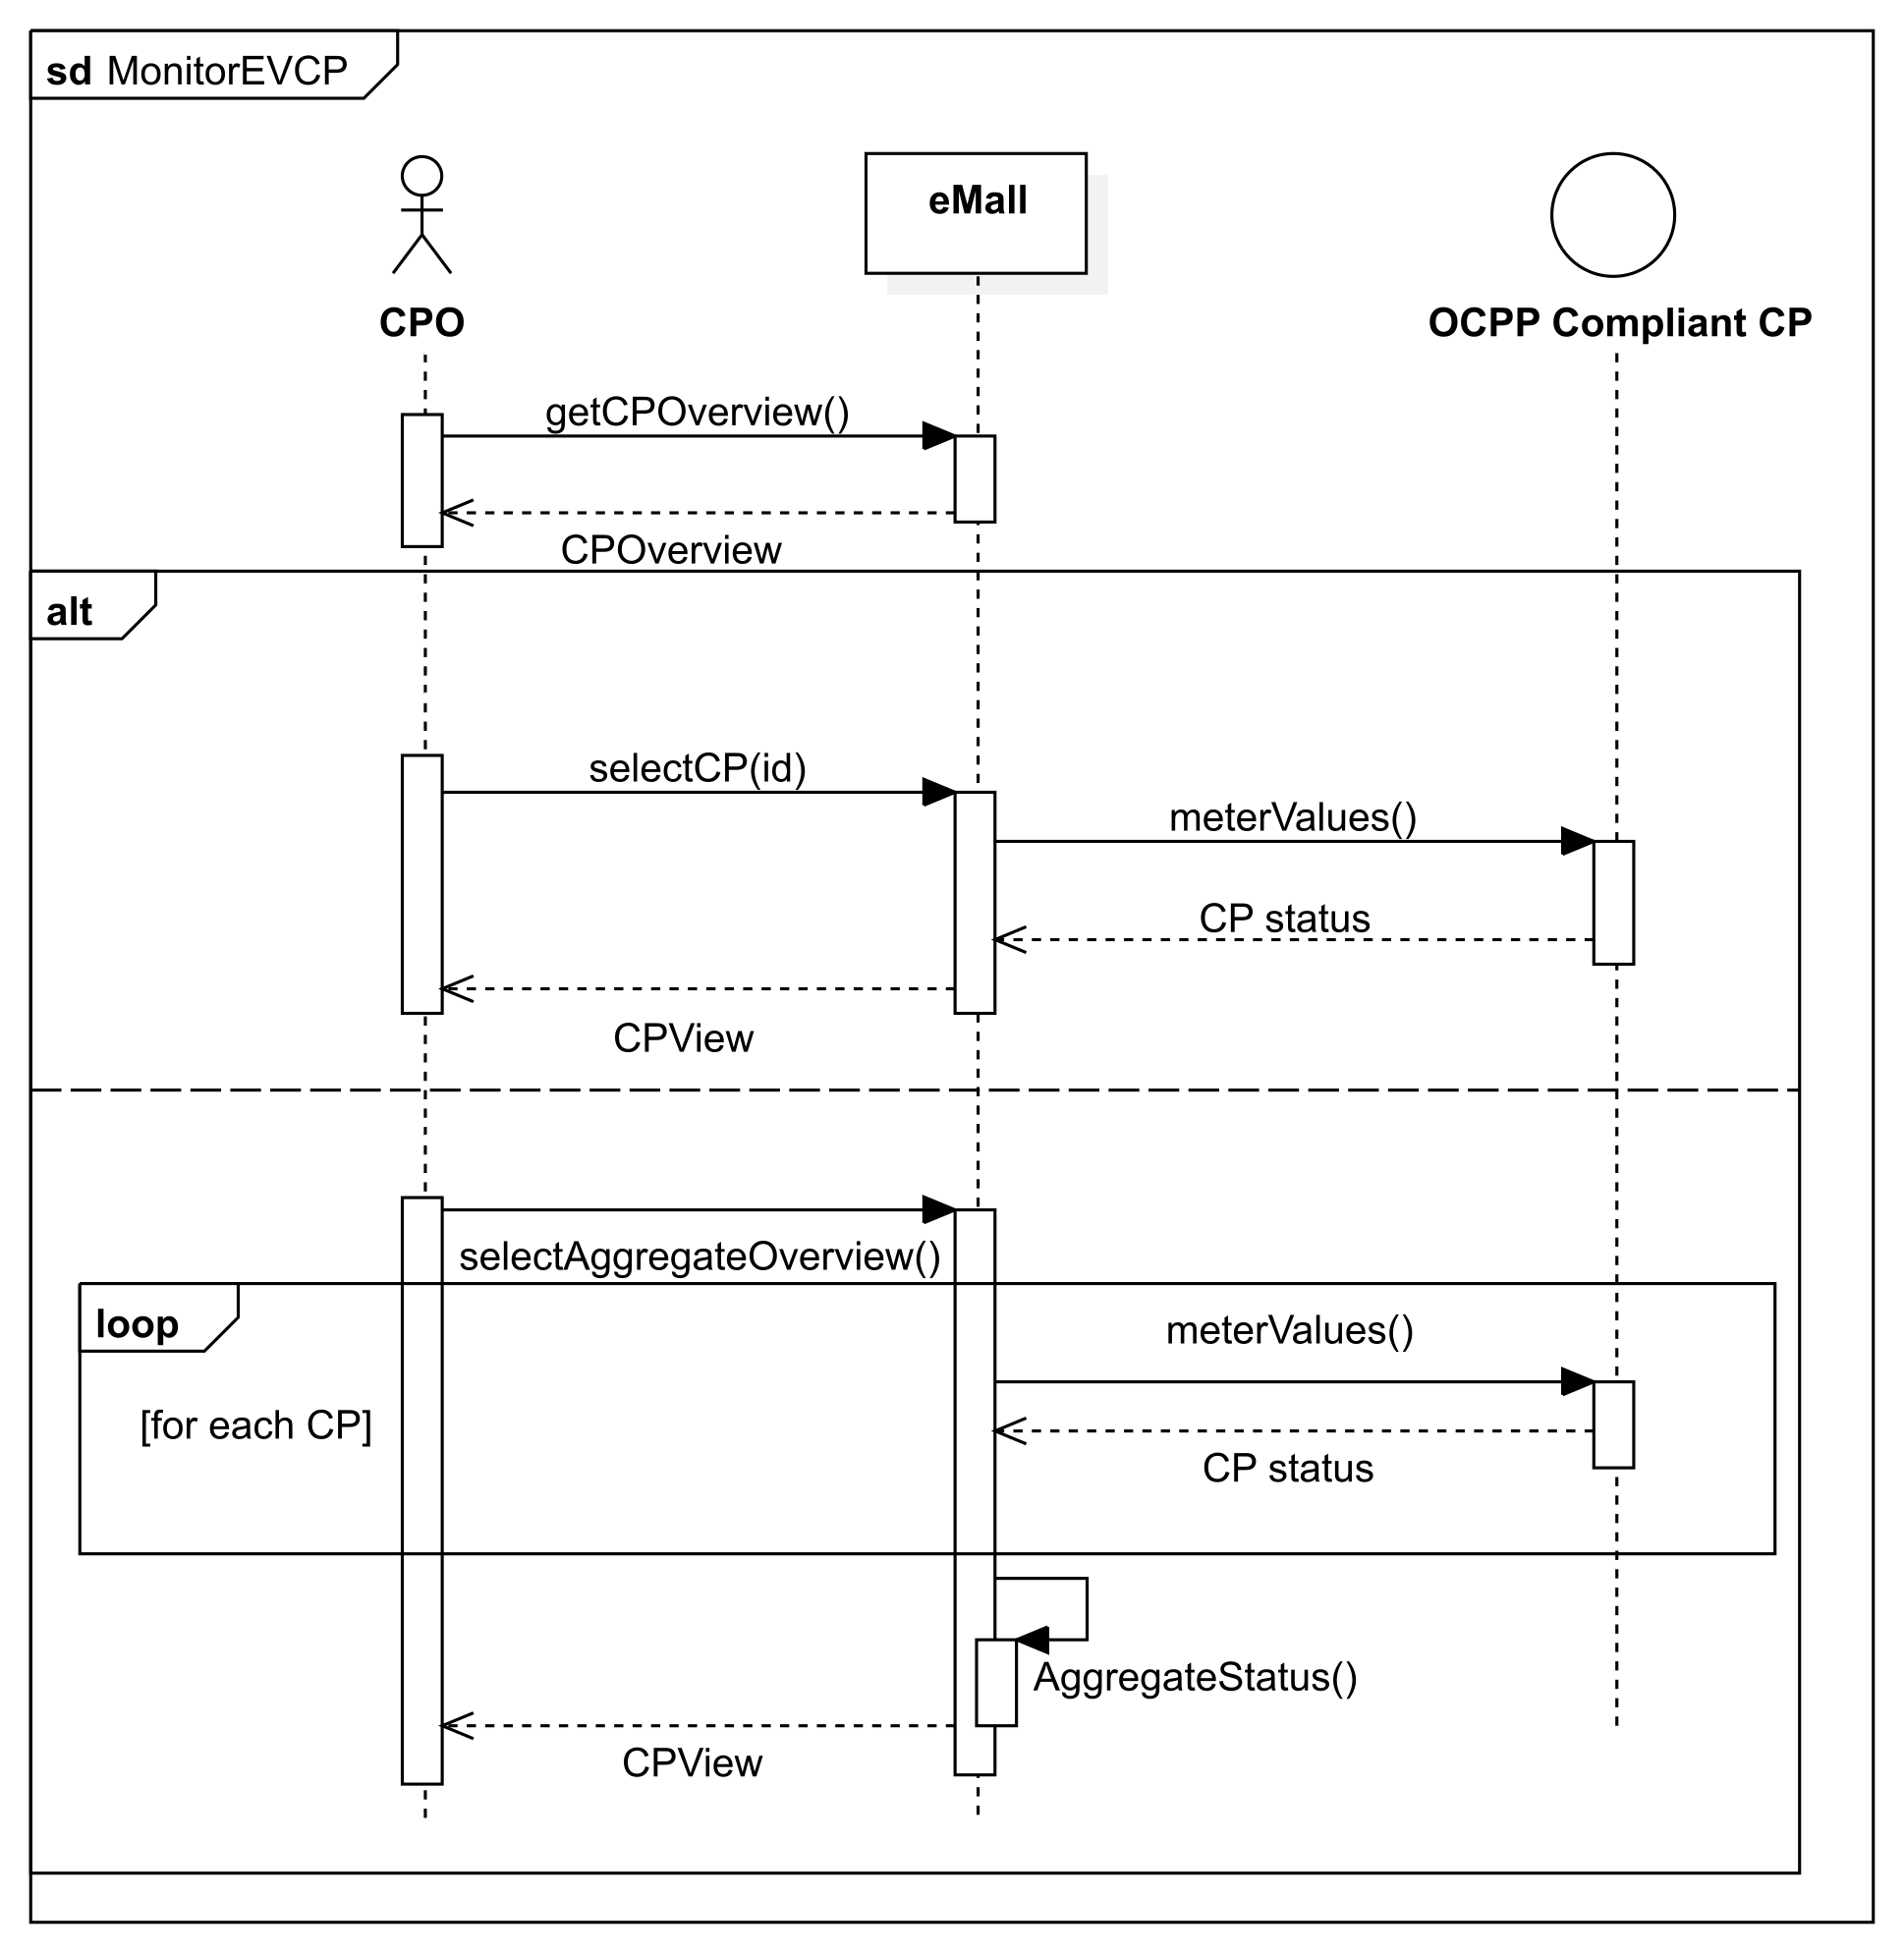
\includegraphics[scale=0.9]{src/sequence_diagram/monitorEVCP.png}
    \end{figure}
}
{11}
{Monitor CPs} % name
{CPO, OCPP compliant CP client} % actor
{Authenticated CPO} % entry condition
{ % event flow
    \begin{enumerate}
        \item The operator clicks "Charging Points" tab
        \item The system asks all the CPs, through OCPP, the details of their status
        \item The CPs reply, through OCPP, with their status
        \item The system shows a table with detailed views of CPs
    \end{enumerate}
}
{The aggregate CPs details charts are displayed} % exit condition
{ % exceptions
    \begin{itemize}
        \item Loss of internet connection
        \item The actor cancels the operation
    \end{itemize}
}
{ % notes
    ...
}

\usecase
{

}
{12.1}
{Monitor specific CP} % name
{CPO, OCPP compliant CP client} % actor
{Authenticated CPO is in "Charging Points" tab} % entry condition
{ % event flow
    \begin{enumerate}
        \item The operator selects a specific CP
        \item The system asks CP, through OCPP, details of its status
        \item The CP replies, through OCPP, with the status
        \item The system shows the details of the chosen CP
    \end{enumerate}
}
{The details of the specific CP are displayed} % exit condition
{ % exceptions
    \begin{itemize}
        \item Loss of internet connection
        \item The actor cancels the operation
    \end{itemize}
}
{ % notes
    ...
}

\usecase
{
    \begin{figure}[H]
        \centering
        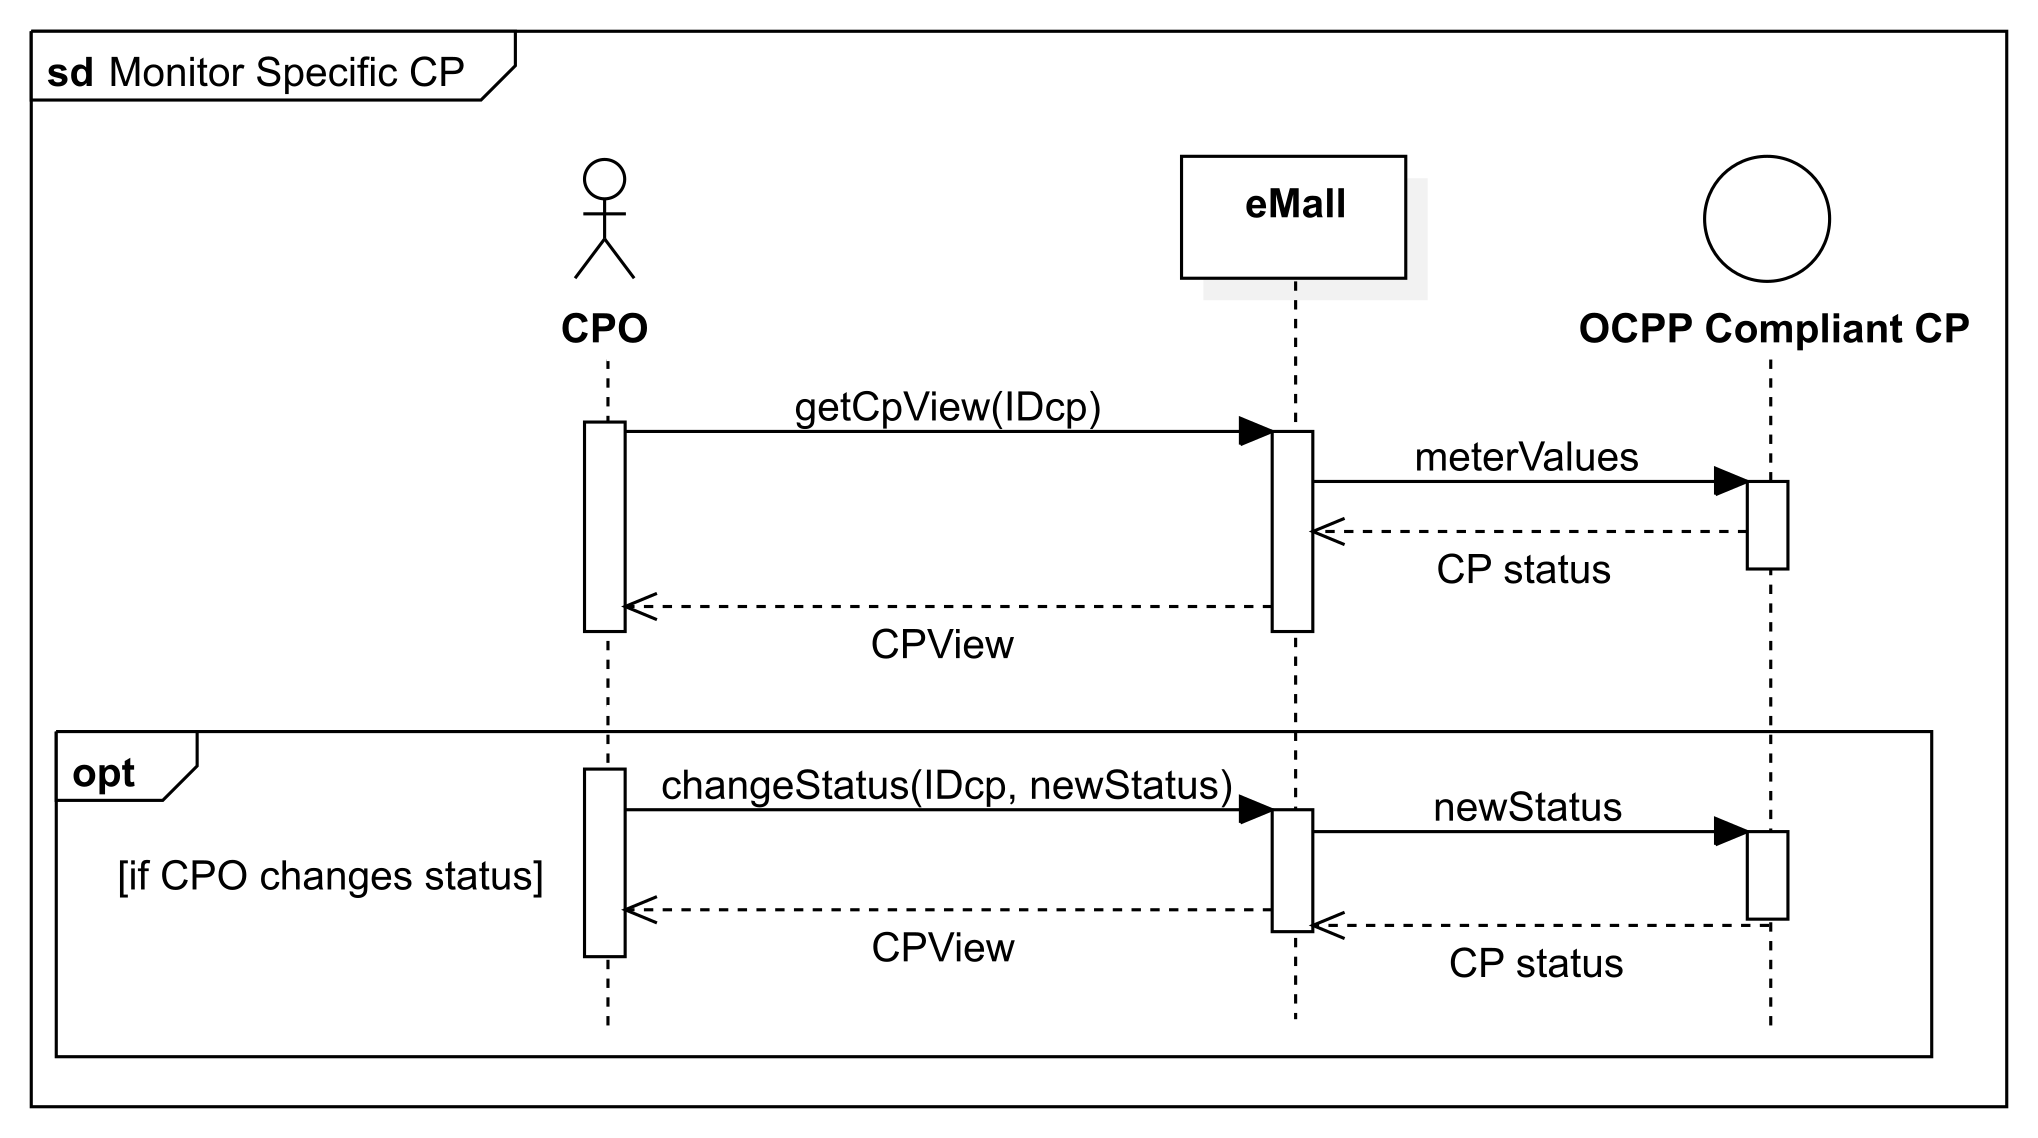
\includegraphics[scale=0.9]{src/sequence_diagram/monitorSpecificCP.png}
    \end{figure}
}
{12.2}
{Change Status of a CP} % name
{CPO} % actor
{Authenticated CPO is in "Charging Point" tab} % entry condition
{ % event flow
    \begin{enumerate}
        \item The operator changes the state of the CP from the provided
        \item The system asks CP, through OCPP, to change to the desired status
        \item The CP replies, through OCPP, with the new status
        \item The system shows the details of the chosen CP
    \end{enumerate}
}
{The change of status of the specific CP has been planned} % exit condition
{ % exceptions
    \begin{itemize}
        \item Loss of internet connection
        \item The actor cancels the operation
    \end{itemize}
}
{ % notes
    ...
}

\pagebreak
\usecase
{
    \begin{figure}[H]
        \centering
        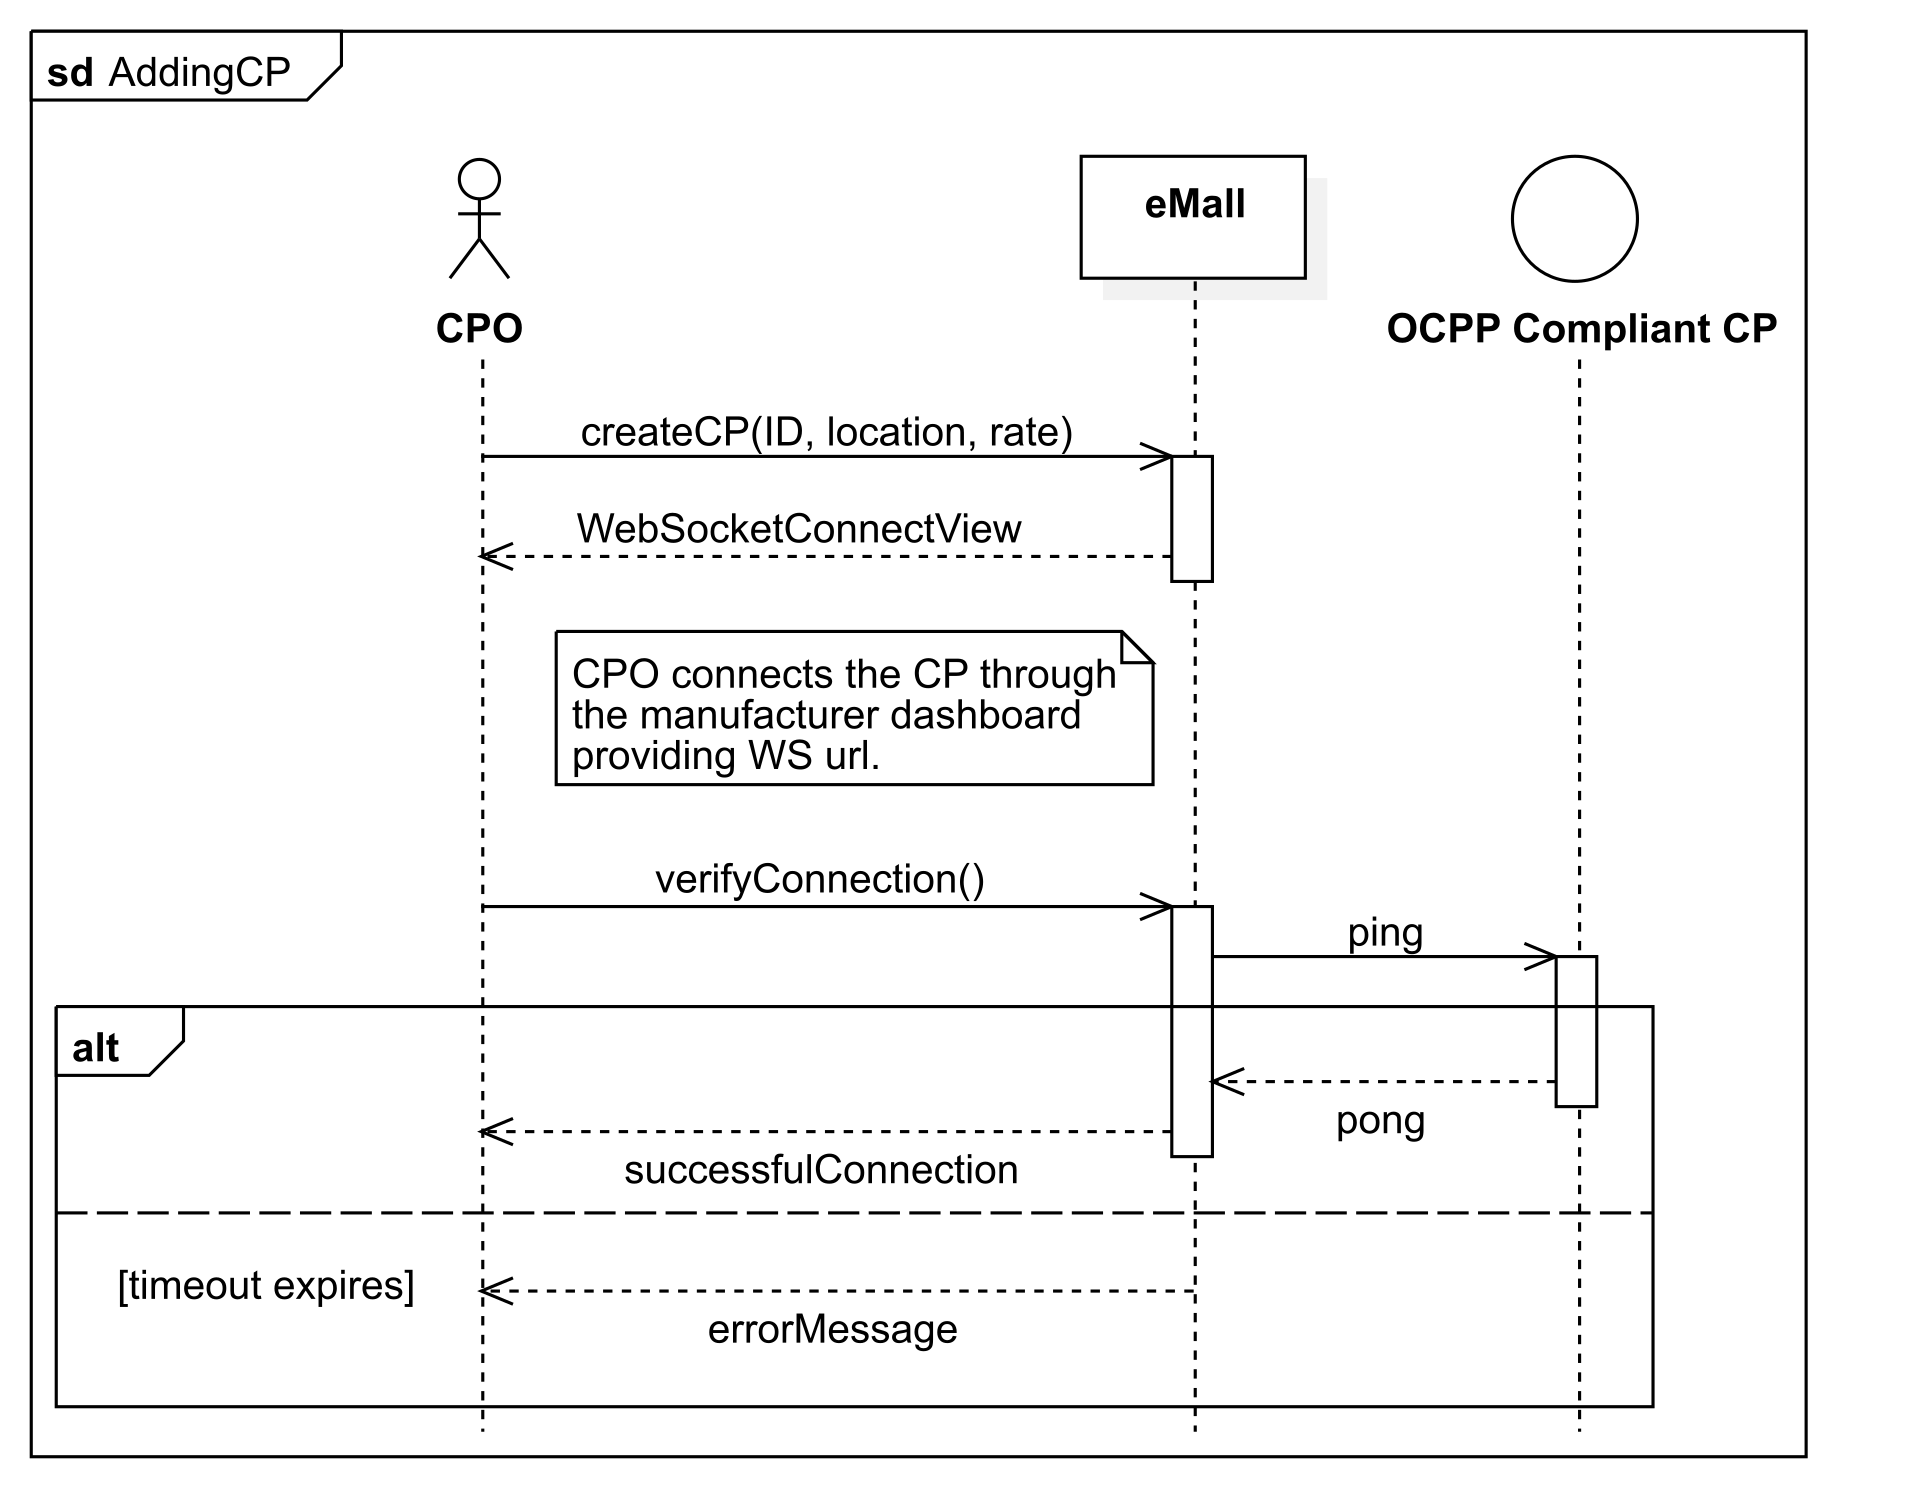
\includegraphics[scale=0.9]{src/sequence_diagram/addingCP.png}
    \end{figure}
}
{13}
{Adding a CP} % name
{CPO, OCPP compliant CP client} % actor
{Authenticated CPO is in "Charging Points" tab} % entry condition
{ % event flow
    \begin{enumerate}
        \item The operator clicks "Add a new CP" button
        \item The system provides a popup to insert details of the new CP
        \item The operator chooses specifies the ID (serial number of CP), the rate that will have to calculate charging costs, the EVCP in which it is, then clicks "connect" button
        \item The system shows an OCPP URL to connect the CP to the CPMS and waits for a connection
        \item The operator connects the CP using the CP's manufacturer platform
        \item The system shows a message when the connection is established
    \end{enumerate}
}
{The new CP is connected} % exit condition
{ % exceptions
    \begin{itemize}
        \item Loss of internet connection
        \item The actor cancels the operation
    \end{itemize}
}
{ % notes
    ...
}

\usecase
{
    \begin{figure}[H]
        \centering
        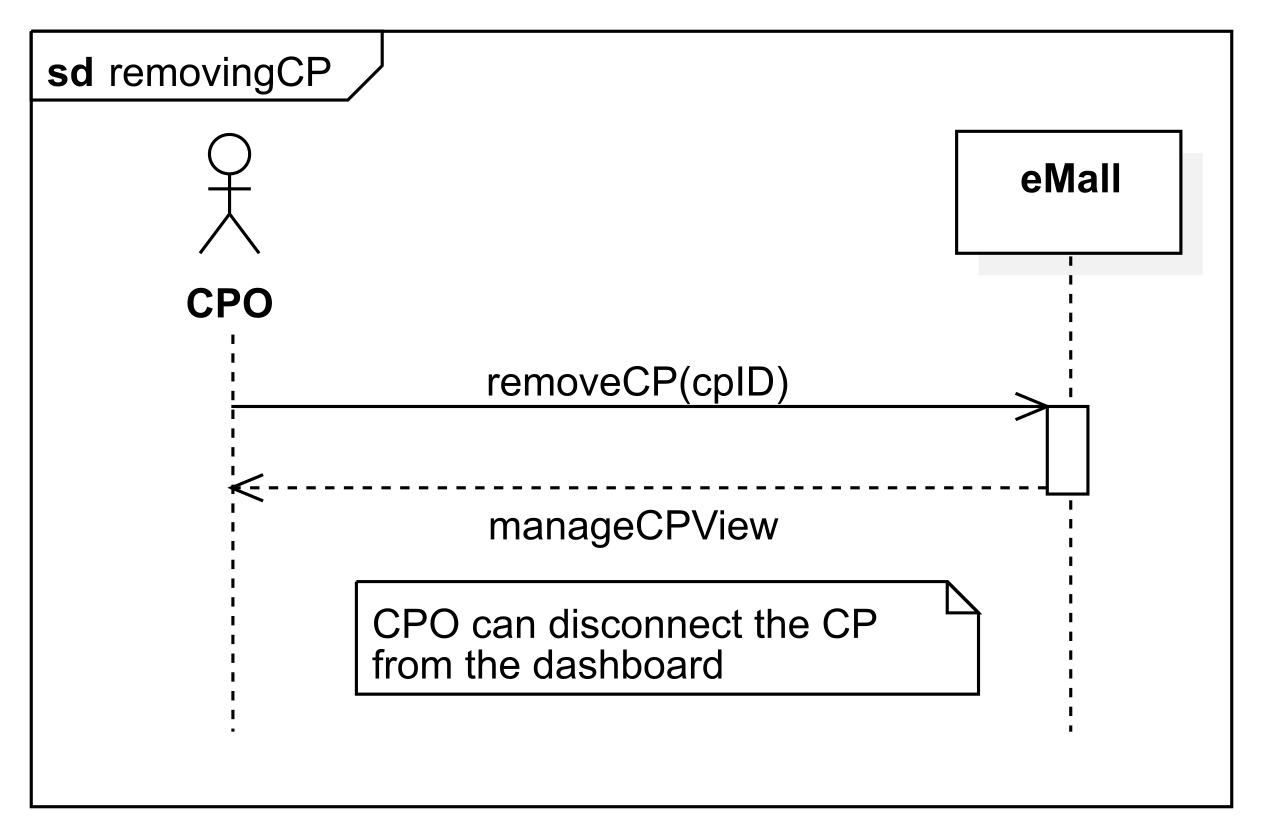
\includegraphics[scale=0.9]{src/sequence_diagram/removingCP.png}
    \end{figure}
}
{14}
{Removing a CP} % name
{CPO} % actor
{Authenticated CPO is in "Charging Points" tab} % entry condition
{ % event flow
    \begin{enumerate}
        \item The operator selects a CP and clicks "Remove CP" button
        \item The system removes the association with the CP
    \end{enumerate}
}
{The CP is removed} % exit condition
{ % exceptions
    \begin{itemize}
        \item Loss of internet connection
        \item The actor cancels the operation
    \end{itemize}
}
{ % notes
    ...
}

\pagebreak
\usecase
{
    \begin{figure}[H]
        \centering
        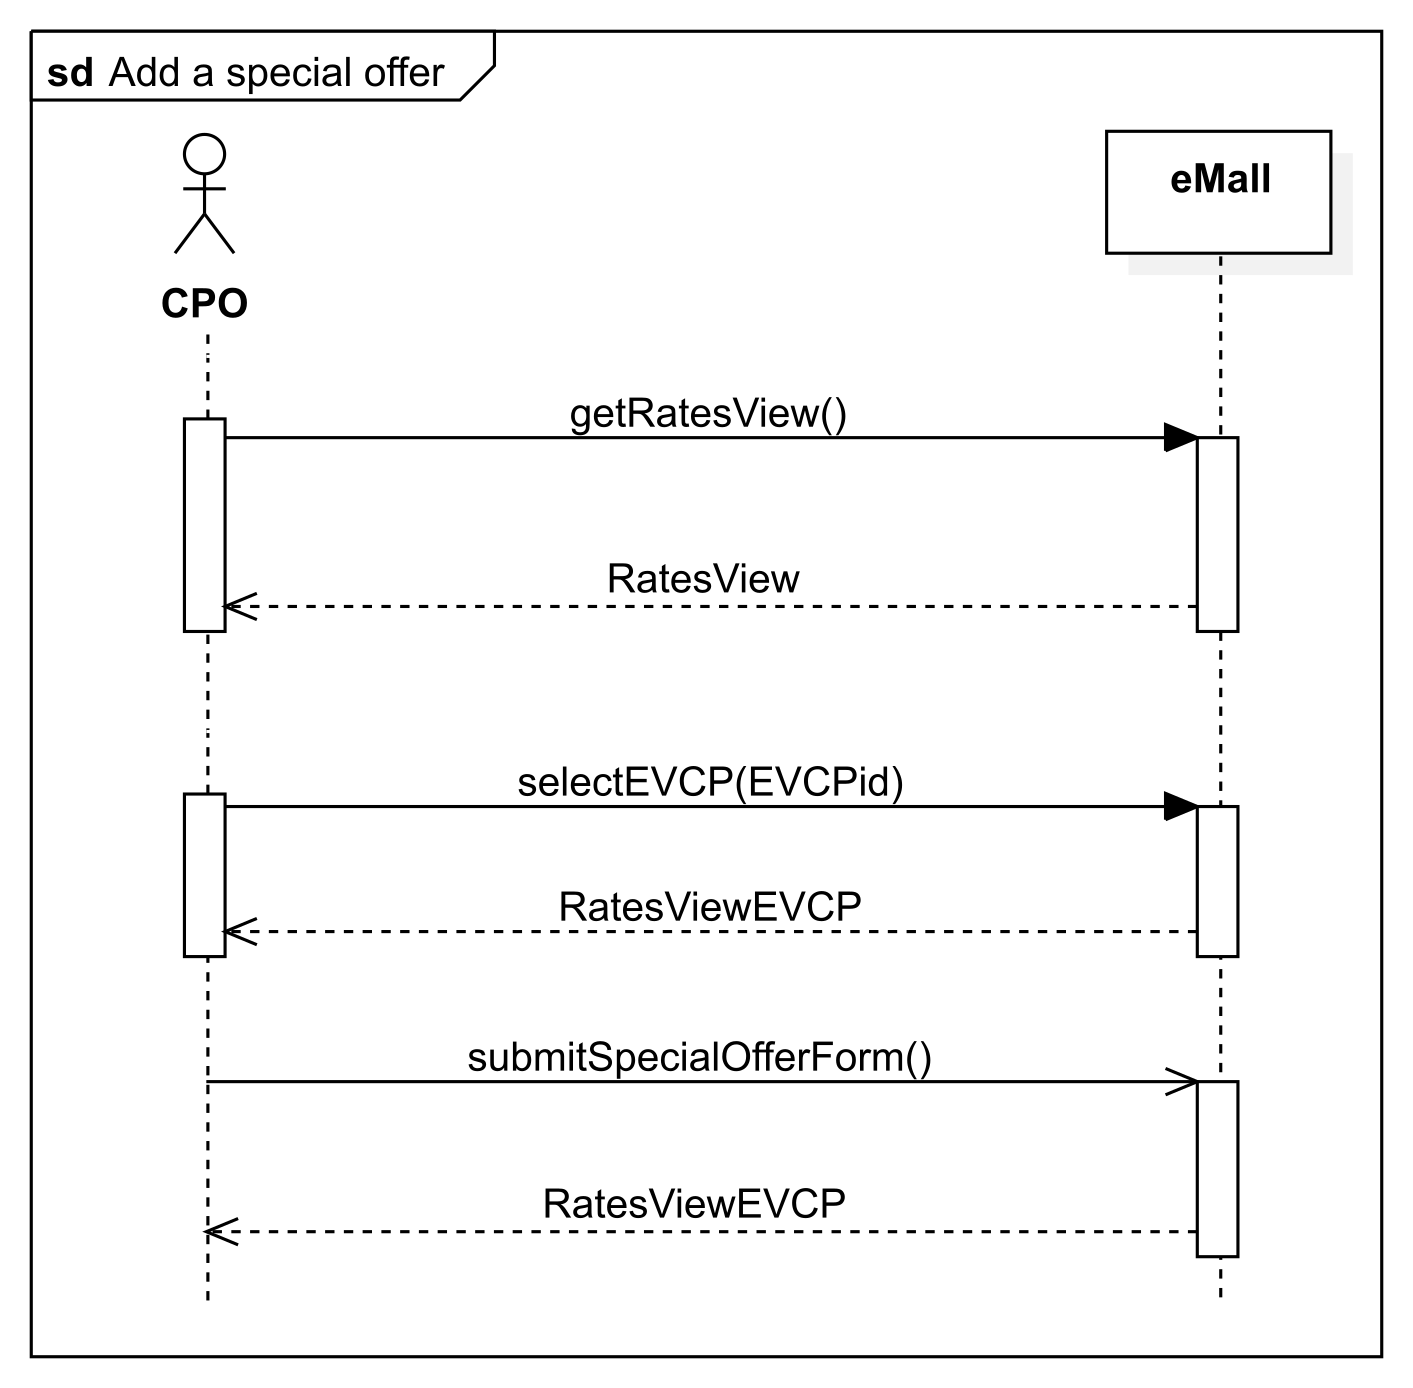
\includegraphics[scale=0.9]{src/sequence_diagram/specialOffer.png}
    \end{figure}
}
{15}
{Add a special offer} % name
{CPO} % actor
{Authenticated CPO is in "Charging Points" tab} % entry condition
{ % event flow
    \begin{enumerate}
        \item The operator chooses a specific EVCP, selects a CP and clicks "Rate" button
        \item The system shows a form in which the operator can select a discount and a time slot or day of the week in which it is valid
        \item The operator fills and submits the form
        \item The system processes the information and shows a success message
    \end{enumerate}
}
{The special offer is created} % exit condition
{ % exceptions
    \begin{itemize}
        \item Loss of internet connection
        \item The actor cancels the operation
    \end{itemize}
}
{ % notes
    ...
}


\usecase
{
    \begin{figure}[H]
        \centering
        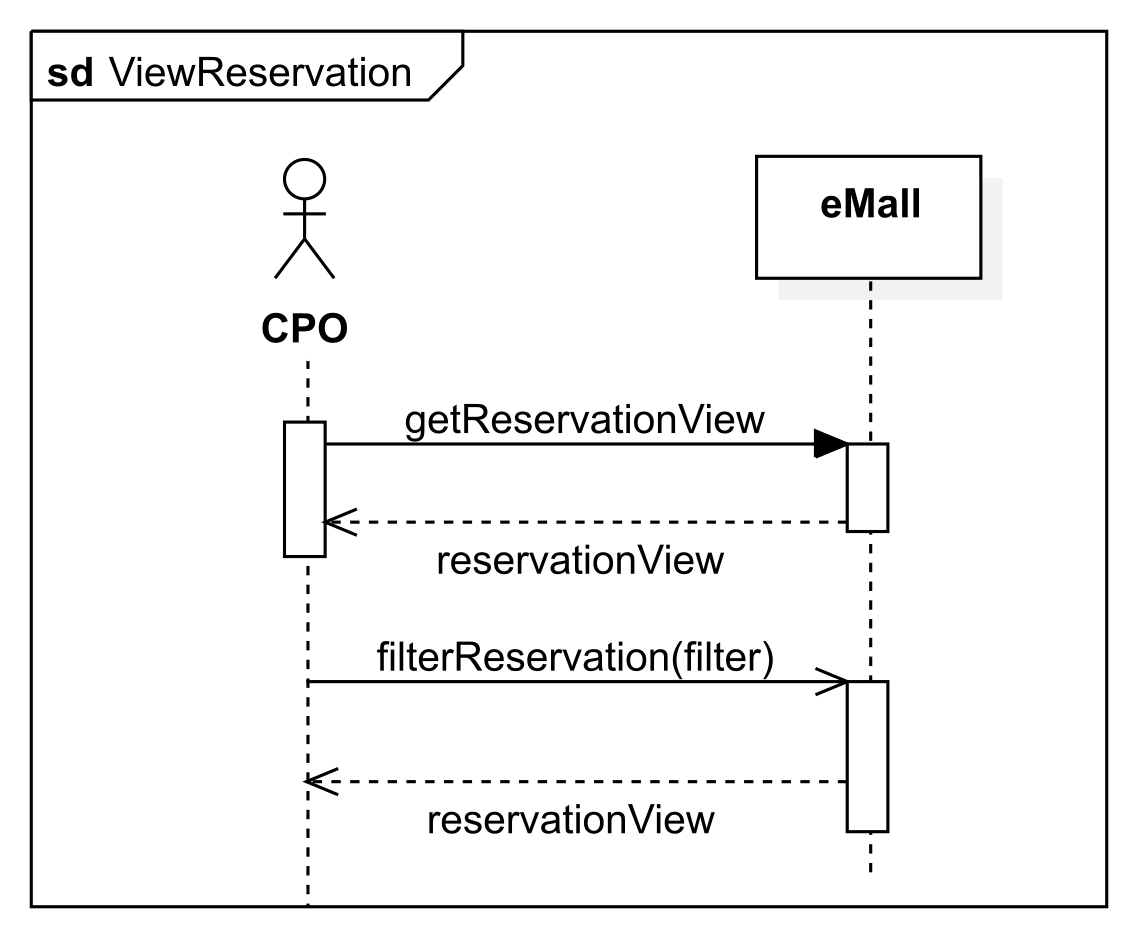
\includegraphics[scale=0.9]{src/sequence_diagram/ViewReservation.png}
    \end{figure}
}
{16}
{View reservations} % name
{CPO} % actor
{Authenticated CPO} % entry condition
{ % event flow
    \begin{enumerate}

        \item The operator clicks "Reservations" tab
        \item The system shows the reservations table
        \item The operator choose a filter (completed, running, pending, upcoming) or to sort reservations (by CP, EVCP, ...)
    \end{enumerate}
}
{The reservations table is displayed} % exit condition
{ % exceptions
    No exception in this use case
}
{ % notes
    ...
}

\pagebreak
\usecase
{
    \begin{figure}[H]
        \centering
        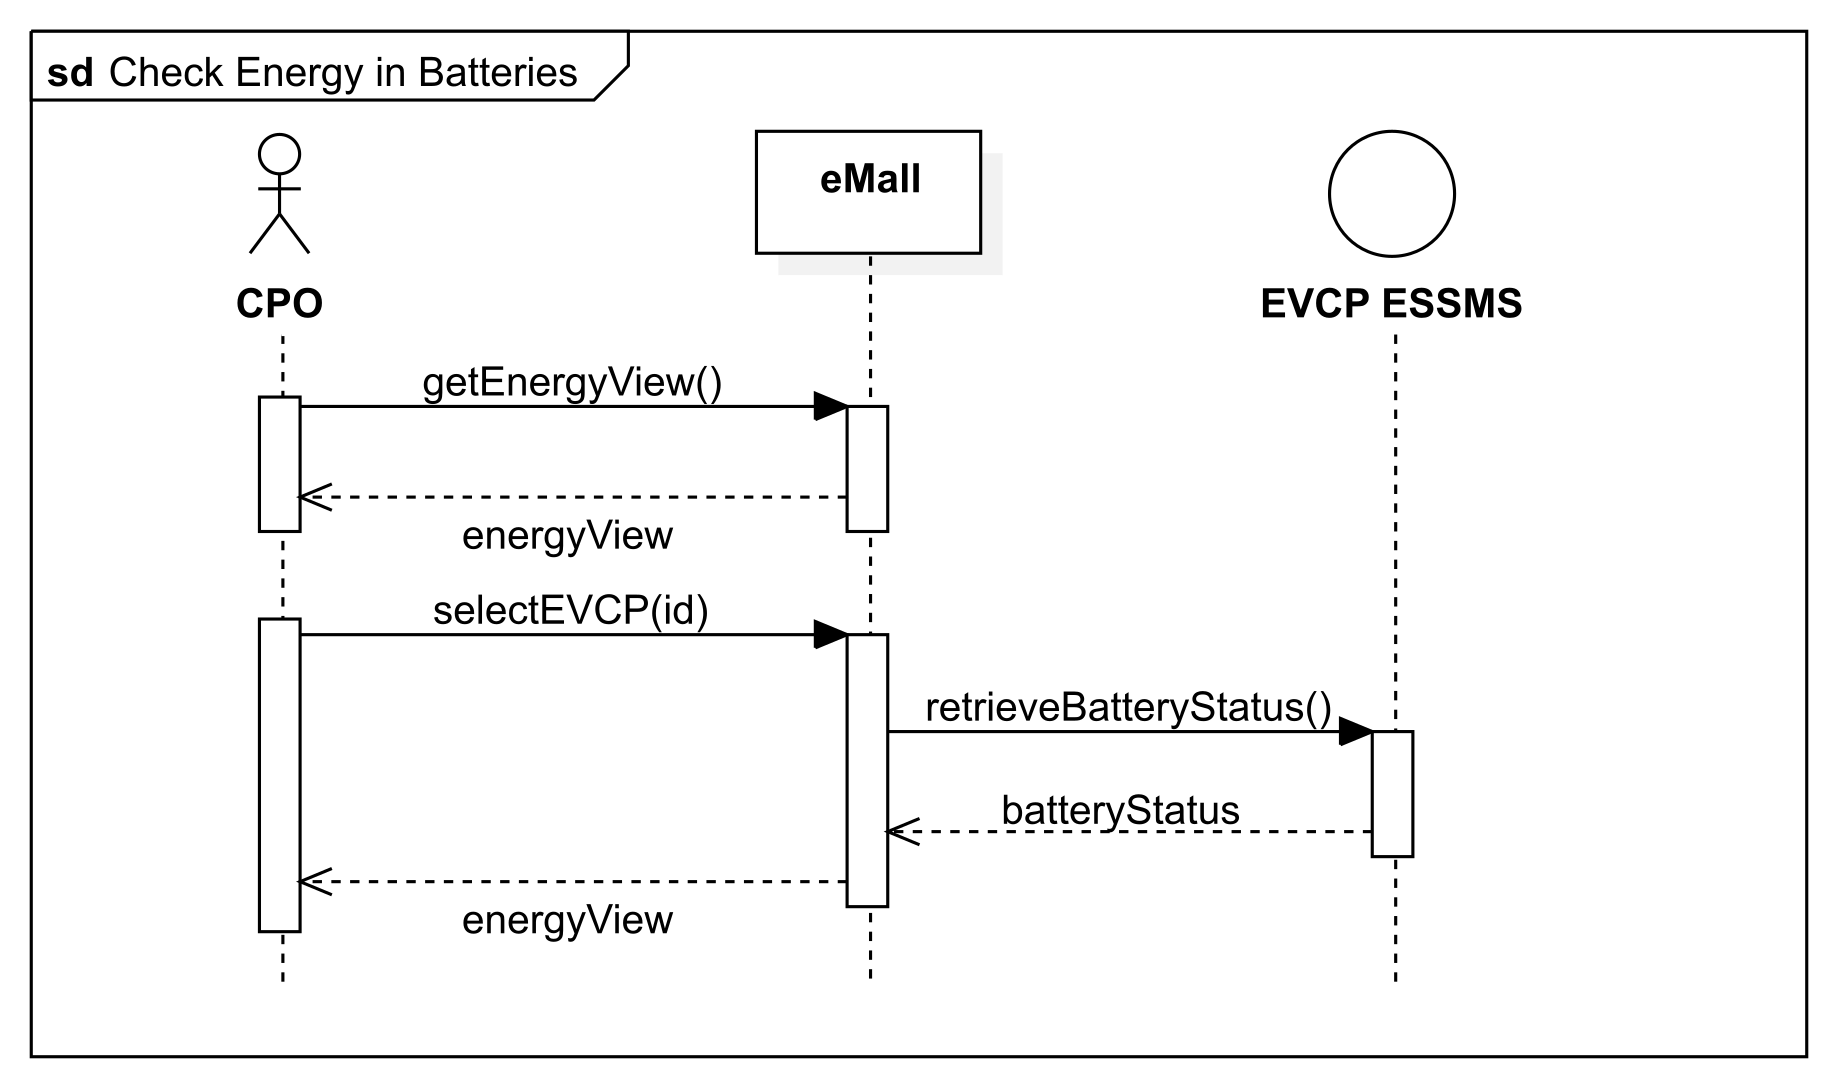
\includegraphics[scale=0.9]{src/sequence_diagram/checkEnergy.png}
    \end{figure}
}
{17}
{Check energy in batteries} % name
{CPO} % actor
{Authenticated CPO is in "Energy" tab} % entry condition
{ % event flow
    \begin{enumerate}
        \item The operator choose a specific EVCP
        \item The system shows the energy storage status of the selected EVCP, if any
    \end{enumerate}
}
{The 'Check energy in batteries' chart is shown} % exit condition
{ % exceptions
    \begin{itemize}
        \item Loss of internet connection
        \item The actor cancels the operation
    \end{itemize}
}
{ % notes
    ...
}

\pagebreak
\usecase
{
    \begin{figure}[H]
        \centering
        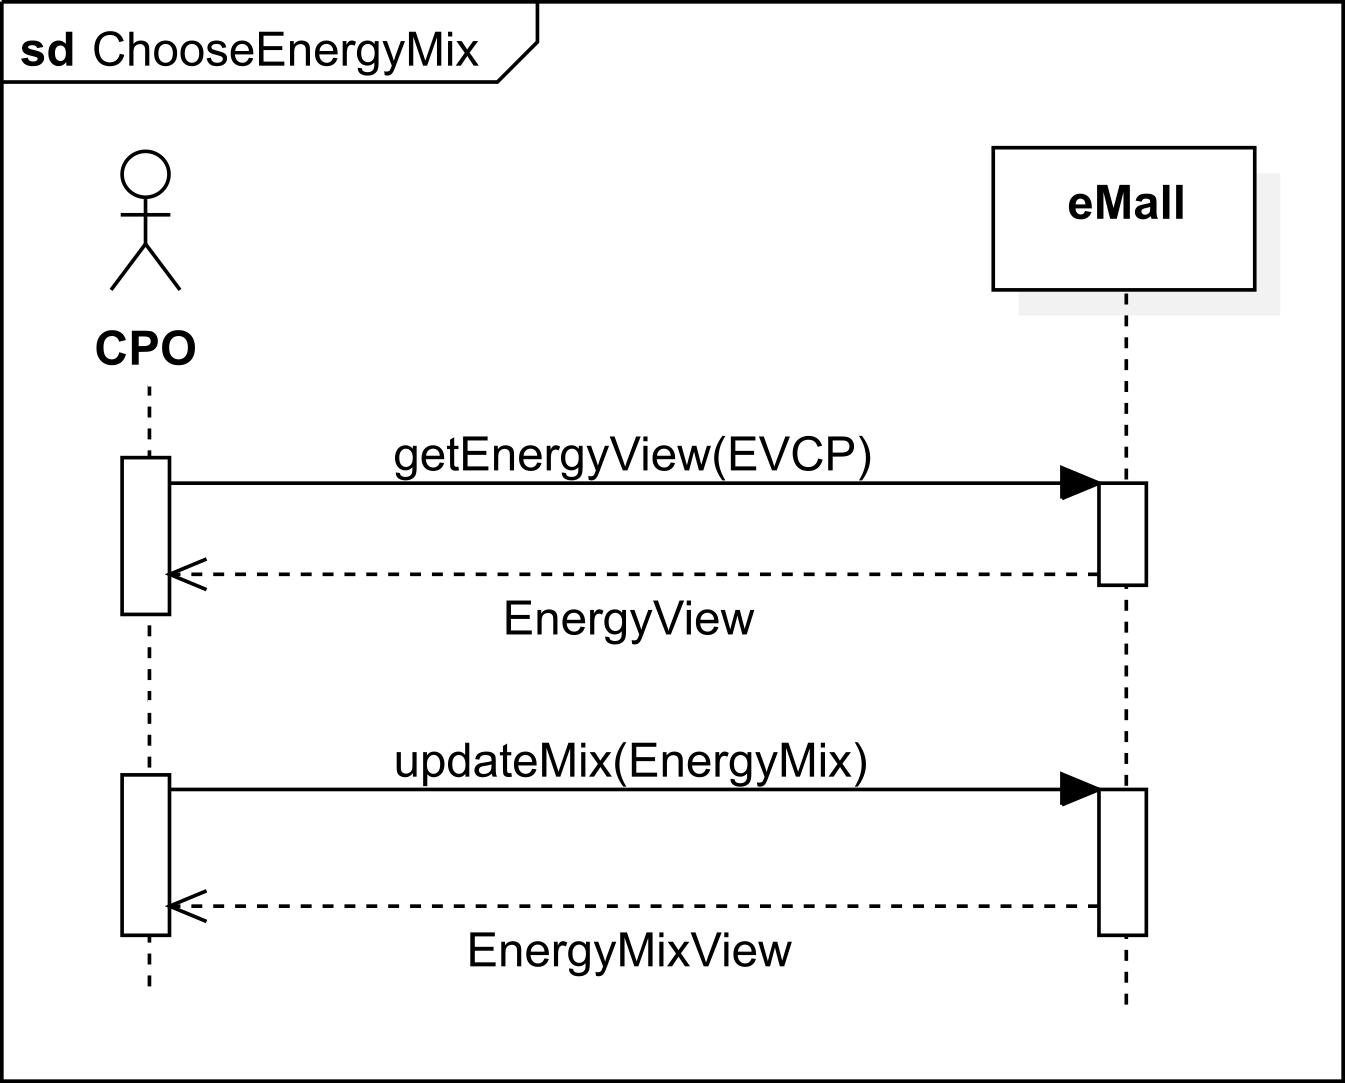
\includegraphics[scale=0.9]{src/sequence_diagram/chooseEnergyMix.png}
    \end{figure}
}
{18}
{Choose energy mix} % name
{CPO} % actor
{Authenticated CPO is in "Energy" tab} % entry condition
{ % event flow
    \begin{enumerate}
        \item The operator chooses a specific EVCP and configure a specific Energy Storage Working Mode
        \item The system processes the information and shows a success message
    \end{enumerate}
}
{The choice of an EVCP energy storing mode is completed} % exit condition
{ % exceptions
    \begin{itemize}
        \item Loss of internet connection
        \item The actor cancels the operation
    \end{itemize}
}
{ % notes
    ...
}




\usecase
{
}
{19.1}
{Retrieve price of energy} % name
{CPO, DSO Energy Price Service} % actor
{Authenticated CPO is in "Energy" tab} % entry condition
{ % event flow
    \begin{enumerate}
        \item The operator choose a specific EVCP
        \item The system asks DSO Energy Pricing Service the list of available DSOs with their prices
        \item The DSO Energy Pricing Service replies with the list requested
        \item The system shows the list of available DSOs with their prices
    \end{enumerate}
}
{The details of price energy are displayed} % exit condition
{ % exceptions
    \begin{itemize}
        \item Loss of internet connection
        \item The actor cancels the operation
    \end{itemize}
}
{ % notes
    ...
}

\usecase
{
    \begin{figure}[H]
        \centering
        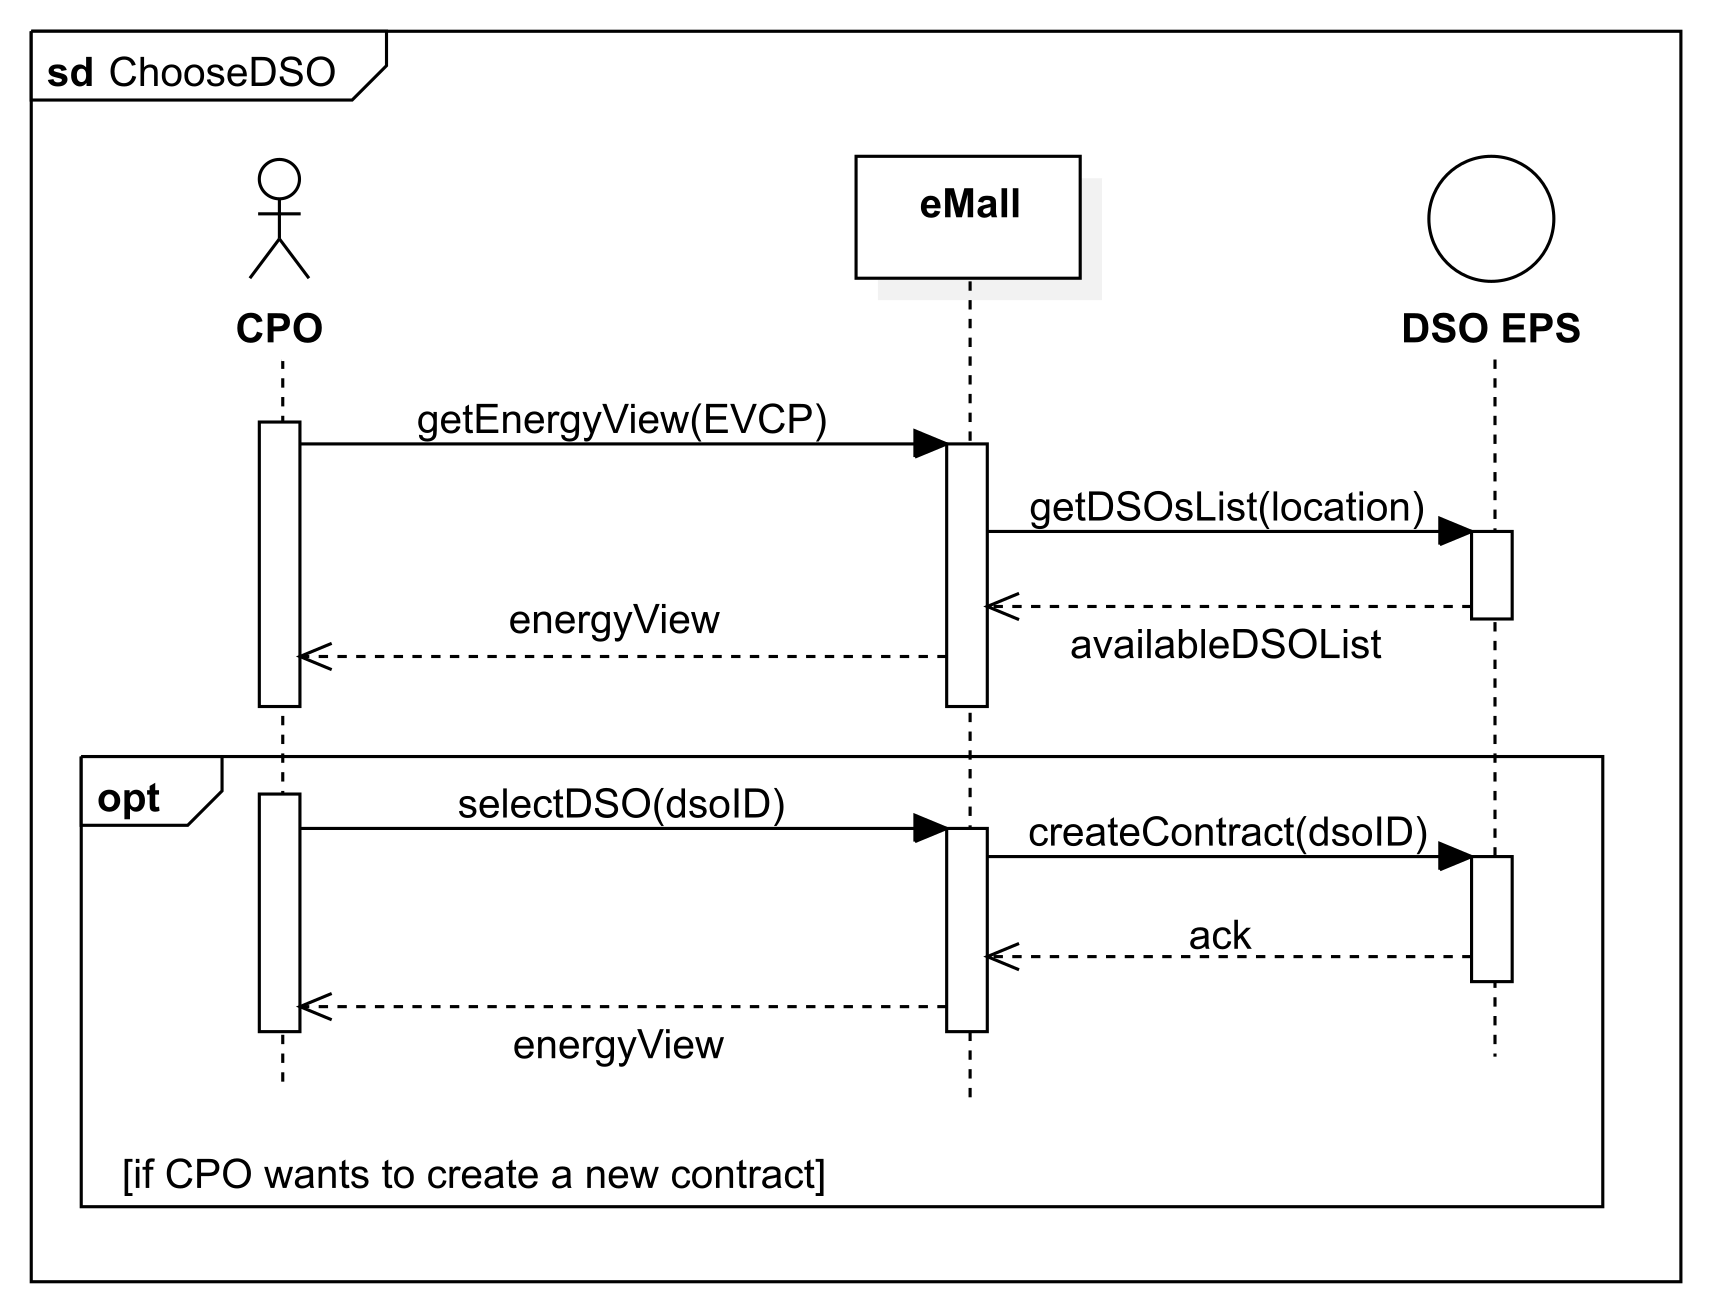
\includegraphics[scale=0.9]{src/sequence_diagram/retrievePrices&chooseDSO.png}
    \end{figure}
}
{19.2}
{Choose DSO} % name
{CPO, DSO Energy Pricing Service} % actor
{Authenticated CPO is in "Energy" tab} % entry condition
{ % event flow
    \begin{enumerate}
        \item The operator choose a specific EVCP, clicks "Change contract"
        \item The operator selects a DSO and submit its choice to the system
        \item The system asks DSO Energy Pricing Service to acquire energy from the chosen DSO for the specified EVCP
        \item The DSO Energy Pricing Service replies with an ACK
        \item The system shows a success message
    \end{enumerate}
}
{The choice of DSO is completed} % exit condition
{ % exceptions
    \begin{itemize}
        \item Loss of internet connection
        \item The actor cancels the operation
    \end{itemize}
}
{ % notes
    ...
}

\pagebreak

\subsubsection{CPO Functional Requirements}
\begin{table}[H]
    \begin{tabularx}{\textwidth}{cX}
        \toprule
        \textbf{R1}  & The system must allow unregistered CPO to register an account                                                                                            \\
        \textbf{R2}  & The system must allow registered CPO to login                                                                                                            \\
        \textbf{R3}  & The system must allow authenticated CPOs making a special offer on their CPs prices                                                                      \\
        \textbf{R4}  & The system must allow authenticated CPOs monitoring the charging process to infer when the battery is full                                               \\
        \textbf{R5}  & The system must allow authenticated CPOs retrieving the amount of energy available in their EVCPs batteries                                              \\
        \textbf{R6}  & The system must allow authenticated CPOs retrieving the number of vehicle being charged in their EVCPs and for each vehicle the amount of absorbed power \\
        \textbf{R7}  & The system must allow authenticated CPOs retrieving the remaining charge time for each connected vehicle                                                 \\
        \textbf{R8}  & The system must allow authenticated CPOs retrieving details on active and historical reservations on their EVCPs                                         \\
        \textbf{R9}  & The system must allow authenticated CPOs acquiring information from the DSOs about the current price of energy                                           \\
        \textbf{R10} & The system must allow authenticated CPOs deciding from which DSO to acquire energy from                                                                  \\
        \textbf{R11} & The system must dynamically decide where to get energy for charging (electrical grid, battery or a mixture)                                              \\
        \textbf{R12} & The system must allow authenticated CPOs statically deciding where to get energy for charging (electrical grid, battery or a mixture)                    \\
        \textbf{R13} & The system must allow authenticated CPOs adding, modifying and deleting CPs                                                                              \\
        \textbf{R14} & The system must allow authenticated CPOs changing availability status of their CPs                                                                       \\
        \bottomrule
    \end{tabularx}
\end{table}
\subsubsection{eMSP Functional Requirements}
\begin{table}[H]
    \begin{tabularx}{\textwidth}{cX}
        \toprule
        \textbf{R15} & The system must allow unregistered users to register an account                                                   \\
        \textbf{R16} & The system must allow registered users to login                                                                   \\
        \textbf{R17} & The system must allow authenticated users to personalize their experience by providing information of their EV    \\
        \textbf{R18} & The system must allow users to search for CPs in the map                                                          \\
        \textbf{R19} & The system must show to the users CPs nearby their current position                                               \\
        \textbf{R20} & The system must allow retrieving details on a given CP regarding connector types supported and cost of the charge \\
        \textbf{R21} & The system must allow authenticated user to book a CP for a certain time interval                                 \\
        \textbf{R22} & The system must allow booking a CP if and only if it is free for the specified time interval                      \\
        \textbf{R23} & The system must notify users when the charging shift is about to start                                            \\
        \textbf{R24} & The system must allow authenticated users to start the charge                                                     \\
        \textbf{R25} & The system must suggest users when and where to charge based on daily schedule, special offers and availability   \\
        \textbf{R26} & The system must allow authenticated users to monitor the charging status                                          \\
        \textbf{R27} & The system must notify authenticated users when the charging process is completed                                 \\
        \textbf{R28} & The system must allow authenticated users to pay for the charge                                                   \\
        \textbf{R29} & The system must allow authenticated users to delete a reservation                                                 \\
        \textbf{R30} & The system must allow authenticated users to view historical reservations                                         \\ \bottomrule
    \end{tabularx}
\end{table}

\subsubsection{Mapping on goals}
\begin{table}[H]
    \begin{tabularx}{\textwidth}{X}
        \toprule
        \textbf{G1} Allow EV driver to plan efficiently their charging process                                                       \\ \midrule
        \textbf{Requirements}                                                                                                        \\ \midrule
        \textbf{R1} The system must allow unregistered CPO to register an account                                                    \\
        \textbf{R13} The system must allow authenticated CPOs adding, modifying and deleting CPs                                     \\
        \textbf{R14} The system must allow authenticated CPOs changing availability status of their CPs                              \\
        \textbf{R15} The system must allow unregistered users to register an account                                                 \\
        \textbf{R16} The system must allow registered users to login                                                                 \\
        \textbf{R18} The system must allow users to search for CPs in the map                                                        \\
        \textbf{R19} The system must show to the users CPs nearby their current position                                             \\
        \textbf{R21} The system must allow authenticated user to book a CP for a certain time interval                               \\
        \textbf{R22} The system must allow booking a CP if and only if it is free for the specified time interval                    \\
        \textbf{R25} The system must suggest users when and where to charge based on daily schedule, special offers and availability \\
        \textbf{R28} The system must allow authenticated users to pay for the charge                                                 \\
        \textbf{R29} The system must allow authenticated users to delete a reservation                                               \\ \midrule
        \textbf{Domain Assumptions}                                                                                                  \\ \midrule
        \textbf{D1} An EV driver arrives at the charging station at a time close to its reservation starting time                    \\
        \textbf{D2} An EV driver leaves the charging station when the charge is finished                                             \\
        \textbf{D3} An EV driver doesn't occupy an already booked charging spot                                                      \\
        \textbf{D5} At least one DSO can always provide energy to the CPOs                                                           \\ \bottomrule
    \end{tabularx}
\end{table}
\begin{table}[H]
    \begin{tabularx}{\textwidth}{X}
        \toprule
        \textbf{G2} Allow EV driver to have a single application for all the processes involving the charge with a personalized experience based on the car and the user commitments \\ \midrule
        \textbf{Requirements}                                                                                                                                                        \\ \midrule
        \textbf{R15} The system must allow unregistered users to register an account                                                                                                 \\
        \textbf{R16} The system must allow registered users to login                                                                                                                 \\
        \textbf{R17} The system must allow authenticated users to personalize their experience by providing information of their EV                                                  \\
        \textbf{R18} The system must allow users to search for CPs in the map                                                                                                        \\
        \textbf{R19} The system must show to the users CPs nearby their current position                                                                                             \\
        \textbf{R20} The system must allow retrieving details on a given CP regarding connector types supported and cost of the charge                                               \\
        \textbf{R21} The system must allow authenticated user to book a CP for a certain time interval                                                                               \\
        \textbf{R23} The system must notify users when the charging shift is about to start                                                                                          \\
        \textbf{R24} The system must allow authenticated users to start the charge                                                                                                   \\
        \textbf{R25} The system must suggest users when and where to charge based on daily schedule, special offers and availability                                                 \\
        \textbf{R26} The system must allow authenticated users to monitor the charging status                                                                                        \\
        \textbf{R27} The system must notify authenticated users when the charging process is completed                                                                               \\
        \textbf{R28} The system must allow authenticated users to pay for the charge                                                                                                 \\
        \textbf{R29} The system must allow authenticated users to delete a reservation                                                                                               \\
        \textbf{R30} The system must allow authenticated users to view historical reservations                                                                                       \\ \midrule
        \textbf{Domain Assumptions}                                                                                                                                                  \\ \midrule
        \textbf{Dep1}  The system requires access to a third party maps API                                                                                                          \\
        \textbf{Dep2}  The system will use the GPS of the driver's computer or smartphone                                                                                            \\
        \textbf{Dep3}  The system will require internet connection to interact with all the users                                                                                    \\
        \textbf{Dep5}  The system will use an external API to retrieve the EV battery status and a list of EV available on the market                                                \\
        \textbf{Dep7}  The system will use an external API to access the calendar of the users                                                                                       \\
        \textbf{Dep8}  The system will use a payment gateway to perform payment operations                                                                                           \\
        \textbf{Dep9}  The system will use an external API to send push notification to the drivers                                                                                  \\
        \textbf{Dep10} The system will use a third party API to send SMS to customers phones                                                                                         \\ \bottomrule
    \end{tabularx}
\end{table}
\begin{table}[H]
    \begin{tabularx}{\textwidth}{X}
        \toprule
        \textbf{G3} Allow CPOs to be reached by EV drivers looking for charging points                                                \\ \midrule
        \textbf{Requirements}                                                                                                         \\ \midrule
        \textbf{R1}  The system must allow unregistered CPO to register an account                                                    \\
        \textbf{R3}  The system must allow authenticated CPOs making a special offer on their CPs prices                              \\
        \textbf{R4}  The system must allow authenticated CPOs monitoring the charging process to infer when the battery is full       \\
        \textbf{R7}  The system must allow authenticated CPOs retrieving the remaining charge time for each connected vehicle         \\
        \textbf{R8}  The system must allow authenticated CPOs retrieving details on active and historical reservations on their EVCPs \\
        \textbf{R13} The system must allow authenticated CPOs adding, modifying and deleting CPs                                      \\
        \textbf{R14} The system must allow authenticated CPOs changing availability status of their CPs                               \\
        \textbf{R15} The system must allow unregistered users to register an account                                                  \\
        \textbf{R16} The system must allow registered users to login                                                                  \\
        \textbf{R18} The system must allow users to search for CPs in the map                                                         \\
        \textbf{R21} The system must allow authenticated user to book a CP for a certain time interval                                \\
        \textbf{R24} The system must allow authenticated users to start the charge                                                    \\
        \textbf{R25} The system must suggest users when and where to charge based on daily schedule, special offers and availability  \\
        \textbf{R27} The system must notify authenticated users when the charging process is completed                                \\
        \textbf{R28} The system must allow authenticated users to pay for the charge                                                  \\ \midrule
        \textbf{Domain Assumptions}                                                                                                   \\ \midrule
        \textbf{D2} An EV driver leaves the charging station when the charge is finished                                              \\
        \textbf{D3} An EV driver doesn't occupy an already booked charging spot                                                       \\
        \textbf{D5} At least one DSO can always provide energy to the CPOs                                                            \\
        \textbf{D6} An user that books a charge has an electric vehicle to charge                                                     \\
        \textbf{D7} An user that books a charge is always reliable                                                                    \\    \bottomrule
    \end{tabularx}
\end{table}
\begin{table}[H]
    \begin{tabularx}{\textwidth}{X}
        \toprule
        \textbf{G4} Provide smart managing of charging stations, including the register of reservations                                                                       \\ \midrule
        \textbf{Requirements}                                                                                                                                                 \\ \midrule
        \textbf{R1}  The system must allow unregistered CPO to register an account                                                                                            \\
        \textbf{R4}  The system must allow authenticated CPOs monitoring the charging process to infer when the battery is full                                               \\
        \textbf{R6}  The system must allow authenticated CPOs retrieving the number of vehicle being charged in their EVCPs and for each vehicle the amount of absorbed power \\
        \textbf{R7}  The system must allow authenticated CPOs retrieving the remaining charge time for each connected vehicle                                                 \\
        \textbf{R8}  The system must allow authenticated CPOs retrieving details on active and historical reservations on their EVCPs                                         \\
        \textbf{R13} The system must allow authenticated CPOs adding, modifying and deleting CPs                                                                              \\
        \textbf{R14} The system must allow authenticated CPOs changing availability status of their CPs                                                                       \\ \midrule
        \textbf{Domain Assumptions}                                                                                                                                           \\ \midrule
        \textbf{D5}    At least one DSO can always provide energy to the CPOs                                                                                                 \\
        \textbf{Dep3}  The system will require internet connection to interact with all the users                                                                             \\
        \textbf{Dep6}  The system will use an external API to retrieve data or send data to the CPs                                                                           \\ \bottomrule
    \end{tabularx}
\end{table}
\begin{table}[H]
    \begin{tabularx}{\textwidth}{X}
        \toprule
        \textbf{G5} Allow CPOs to choose between contracts of energy providers and to determine the energy source mix                                      \\ \midrule
        \textbf{Requirements}                                                                                                                              \\ \midrule
        \textbf{R5}  The system must allow authenticated CPOs retrieving the amount of energy available in their EVCPs batteries                           \\
        \textbf{R9}  The system must allow authenticated CPOs acquiring information from the DSOs about the current price of energy                        \\
        \textbf{R10}  The system must allow authenticated CPOs deciding from which DSO to acquire energy from                                              \\
        \textbf{R11} The system must dynamically decide where to get energy for charging (electrical grid, battery or a mixture)                           \\
        \textbf{R12} The system must allow authenticated CPOs statically deciding where to get energy for charging (electrical grid, battery or a mixture) \\  \midrule
        \textbf{Domain Assumptions}                                                                                                                        \\ \midrule
        \textbf{D5}   At least one DSO can always provide energy to the CPOs                                                                               \\
        \textbf{Dep3} The system will require internet connection to interact with all the users                                                           \\
        \textbf{Dep4} The system will use an external API to retrieve the prices of energy by the available DSOs                                           \\  \bottomrule
    \end{tabularx}
\end{table}
\subsubsection{Mapping on use cases}
\begin{table}[H]
    \begin{tabularx}{\textwidth}{XXX}
        \toprule
        \textbf{Use Case}                             & \textbf{Requirements} \\ \midrule
        U1 - Login                                    & R2 R16                \\
        U2 - Registration                             & R1 R15                \\
        U3 - Map Filtering                            & R18 R19               \\
        U4 - EVCP Details                             & R20                   \\
        U5 - Book a Charge                            & R21 R22 R28           \\
        U6 - Start a Charge                           & R24                   \\
        U7 - Insert Car Details                       & R17                   \\
        U8 - (EV Driver) History of Reservation       & R26 R30               \\
        U9 - Details of the current charge            & R26                   \\
        U10 - Delete a reservation                    & R29                   \\
        U11 - Monitor CPs                             & R4 R6 R7              \\
        U12 - Monitor Specific CP and Change Status   & R14                   \\
        U13 - Adding a CP                             & R13                   \\
        U14 - Removing a CP                           & R13                   \\
        U15 - Add a special offer                     & R3                    \\
        U16 - (CPO) View reservation                  & R8                    \\
        U17 - Check energy in batteries               & R5                    \\
        U18 - Choose energy mix                       & R11 R12               \\
        U19 - Retrieve price of energy and Choose DSO & R9 R10                \\
        \bottomrule
    \end{tabularx}
\end{table}

\subsection{Performance Requirements}
To guarantee the best possible experience to both EV drivers and CPOs, the system should:
\begin{itemize}
    \item provide a scalable, reactive and capable of load-balancing backend
    \item assure protection against DDoS attacks
    \item provide a responsive and fluid frontend. The frontend must handle correctly asynchronous interactions
          with the server, even when the connection quality is bad, in order to provide the best possible experience
    \item push notification with a delay that is imperceptible to the user
    \item be able to handle a number of users that increases with the growth of the EV market. As shown in previous statistics in the Introduction, in 2021 the number of EV in use worldwide was about 16498750 units. About 6 million EV are on the roads in Europe. The system must be capable of handling initially at least 500000 users and 75000 peak concurrent users
\end{itemize}

\subsection{Design Constraints}


\subsubsection{Standards compliance}
Specifications described in this document must be respected by the system.
Source code of the application must be commented on and documented adequately.
The system should respect the guidelines described by the GDPR.

\subsubsection{Hardware limitations}
The system requires any device and a stable internet connection.

\subsection{Software System Attributes}
\subsubsection{Reliability}
In order to guarantee better reliability performances, all
the scheduled maintenance of the system should be done during
the night.
It should also be noted that some functionality of the system relies on external APIs, though the system should not completely fail
because of failure in one of those. It's also important to avoid data loss through redundant storage methods.

\subsubsection{Availability}
The system should offer its functionalities with an availability
equal to 99.5\%, or more. In other words, the system must be inaccessible
for less than two days every year. To achieve this goal, the system should
provide a high redundancy for the most critical components.


\subsubsection{Security}
To protect users sensible data the system must collect the minimum data possible, and store them in an encrypted database.
The connection between the application must follows modern standard protocols as HTTPS. Do note that not only phone number and password should be considered as sensible data, but also users location, EV details and reservations.
Moreover, all passwords must be salted and encrypted.

\subsubsection{Maintainability}
Source code and correlated documentation must be commented and kept updated.
Modularity, low coupling and high cohesion between components must be a focus during the
designing and developing phases. In particular modularity of the frontend and backend must allow developers to update the backend without users even noticing it.

\subsubsection{Portability}
The application must be available on major mobile OSs targeting at least the current
release. The web application must run at least on the most recent
browsers. It would be a smart choice to reuse most of the codebase
across mobile and web by using cross platform tools.

\subsubsection*{Summary of Non Functional Requirements}
\begin{table}[H]
    \begin{tabularx}{\textwidth}{cX}
        \toprule
        \textbf{NFR1} & The backend of the system must be scalable and flexible (e.g. allocate resources based on the users to be served) to support a variable number of users over time \\
        \textbf{NFR2} & The frontend of the system must be responsive, fluid and easy to use                                                                                              \\
        \textbf{NFR3} & The system must respect the guidelines of the GDPR                                                                                                                \\
        \textbf{NFR4} & The availability of the system must be greater or equal to 99.5\%                                                                                                 \\
        \textbf{NFR5} & The system must collect the minimum amount of data possible and encrypt those data                                                                                \\
        \textbf{NFR6} & The system must be easily maintainable                                                                                                                            \\
        \textbf{NFR7} & The system must be usable on modern browsers and major mobile OSs                                                                                                 \\
        \bottomrule
    \end{tabularx}
\end{table}